\documentclass[11pt]{report}
\usepackage{projectreport}

\newcommand{\name}{John W. Holden}
\newcommand{\course}{Doctor of Philosophy}
\newcommand{\projecttitle}{Mathematical and Computational Modelling of Infectious Tree Diseases}
\newcommand{\submissiondate}{September 2020}
\newcommand{\submissionyear}{2020}

\setcounter{tocdepth}{4}
\setcounter{secnumdepth}{4}
\begin{document}

\maketitle

\chapter*{Intellectual Property}
\addcontentsline{toc}{chapter}{Intellectual Property}
The candidate confirms that the work submitted is his/her own and that appropriate credit has been given where reference has been made to the work of others.

This copy has been supplied on the understanding that it is copyright material and that no quotation from the thesis may be published without proper acknowledgement.

© \submissionyear\ The University of Leeds, \name

\vspace{2cm}
Signed 
\makebox[4cm][c]{\raisebox{-2ex}{\includegraphics[width=3cm, height=1cm]{example-image}}} % replace with your signature

\chapter*{Acknowledgements}
\addcontentsline{toc}{chapter}{Acknowledgements}
This research has been carried out by a team which has included (name the individuals). My own contributions, fully and explicitly indicated in the thesis, have been......(please specify)” The other members of the group and their contributions have been as follows: (please specify).

\chapter*{Abstract}
\addcontentsline{toc}{chapter}{Abstract}

Presently, tree populations worldwide face unprecedented threats from invasive pests and pathogens endangering ecological function, timber production and human wellbeing. 
From first principles, this thesis incrementally extends a simple percolation model of forest-based epidemics into a more involved stochastic dispersal framework combined with host data. 
% The research aims to construct robust epidemic models of tree disease over the landscape of Great Britain and afterwards optimise a novel epidemic control strategy.
The approach developed here couples two spatially-explicit epidemic models at different scales. 
First, a non-local stochastic model of pathogen dispersal between trees is constructed. 
Then, the small-scale epidemic model is projected onto a large-scale distribution of host abundance, resulting in an $R_0$-map across Great Britain. 
Subsequently, a clustering algorithm is employed to identify high-risk regions in the $R_0$-map. 
Initial results indicate a global epidemic phase transition across the distribution, conditional on an infectivity parameter.
The approach to `spatially scale' an epidemic model over the entire landscape is computationally efficient, flexible and adaptable to many pests and pathogens. 
Numerous studies have sought to understand and optimise epidemic control in botanical populations. 
The mainstream control paradigm generally seeks to optimise an `eradication radius' about infected symptomatic trees over a relatively small spatial scale. However, large-scale epidemic control based solely on the spatial distribution of hosts has yet to be explored in depth. 
As such, this thesis will also examine how host heterogeneity, combined with targeted epidemic control, can give rise to natural `pinch-points' that may slow the epidemic spread between regions. 
Ultimately, this investigation intends to help policymakers reach informed decisions about where to focus control in the landscape of Great Britain.

% Ultimately, this investigation intends to help policymakers reach informed decisions about \textit{where} to focus control in the landscape.

\newcommand{\RNum}[1]{\uppercase\expandafter{\romannumeral #1\relax}}
. % abstract + intellectual property + acknowledgements

\tableofcontents  % --> customize this...
\listoffigures
\listoftables
\gls{alb} \gls{acb} \gls{cca} \gls{com} \gls{slm}  \gls{adb} \gls{opm}
\printglossary[title={Abbreviations},type=acronym,style=long]
\newpage
\setcounter{page}{0}
\pagenumbering{arabic}

% Uncomment to see chapter:
% \chapter{Introduction and Literature Review}

This study will outline how to construct models of infectious tree disease for the purpose of epidemic control. Starting from a simple, parsimonious mathematical model of tree disease and limited information on parameter-values, I will show how to construct more elaborate models. As we move from simple model definitions, based on a uniform lattice, this thesis rigorously accesses limiting assumption in the model at each step as we move towards a more elaborate and sophisticated model. From a well constructed model, optimal large-scale epidemiological control will be investigated in an attempt to help inform policy makers about the best decision of resource expenditure and control efficiency. Throughout this study, I hope to provide useful techniques to capture and quantify the spread of disease through a population of trees.\\

This introductory chapter serves to inform the reader about the background, societal importance and modelling paradigms used in tree-based epidemiology. Firstly, the background and motivation for understanding tree disease will be reviewed. After which, a historical perspective will be outlined and I will conduct a through review into the various types of approaches that can be used to model the spread of disease through a population of trees. To this aim, several key concepts will be reviewed, including the basic reproduction number for plant-based diseases, the role of scale in transmission and dispersal. \newpage

\section{Background and Motivation}

In this study, I will focus on the mathematical and computational modelling tree-based epidemics in Great Britain. The problem of tree disease is vast and multifaceted, in reality, a country is likely to be effected by multiple threats involving diverse species of host and pathogen. Managing any a single outbreak is in itself an ambitious task, let alone managing simultaneous outbreaks on several fronts. However, we proceed.\\

\subsection{Trees-health and ecosystem function}
\begin{itemize}
    \item \textcolor{red}{I could expand on the economics, along with climatic and ecological importance of trees}
\end{itemize}
Trees grow naturally, in both rural and urban settings, this includes commercially managed plantations and orchards. Protecting and ensuring tree-health is of essential importance for society \cite{Boyd1235773}. Trees play a central role in terrestrial ecosystems \cite{boyd2013consequence} and their importance of forestry health is widely recognised. The motivations to protect tree populations in rural and urban landscapes are numerous. The most widely known, and well researched, themes include economic, climatic and ecological function \cite{freer2017tree}. However, the benefits of maintaining tree-health also stretch into of realms of human well-being, mental health, recreation and the perception of natural beauty \cite{tyrvainen2005benefits}. See Table \ref{table:tree-health} for a brief overview of the different benefits tree-health can offer to ecosystem and ecosystem function.\\

\subsection{The problem of tree diseases}
\begin{itemize}
    \item \textcolor{red}{I could expand on the biology of pests and pathogens and their interactions with trees}
\end{itemize}
% pest, pathogens and how they effect tree-health
Standing in the way of tree-health and ecosystem-function is the spread of disease through pest and pathogen vectors. Tree populations are subject to infection, the spread of disease and death just like human populations \cite{hethcote2000mathematics}. The main drivers of tree-based epidemics consist of fungi, bacteria, virus, oomycetes and instects \cite{manion1981tree}. To model the spread of tree disease, we require a sound knowledge of the general biological interactions involved. Thus, it is necessary to understand some distinctions between pests and pathogens and introduce some important examples and nomenclature.\\

The terms `pest' and `pathogen' are both broad referring to taxonomically diverse organisms. A pest is defined as any organism that harms humans or human interests such as crops or livestock \cite{oerke2006crop, de1964biological, buckle2015rodent}. The main pest-threats to tree species are typically insects \cite{metcalf1994introduction}. As an example, the Asian longhorn beetle (ALB) \cite{haack2010managing} and oak processionary moth OPM \cite{tomlinson2015managing} are two pests that currently threaten trees in Great Britain. On the other hand, an organism is a pathogen if it causes disease \cite{balloux2017q}. In the context of tree disease this includes fungi, bacteria, virus, oomycetes \cite{Boyd1235773}. In Great Britain, \textit{Phytophthora ramorum} \cite{brasier2005phytophthora} and Ash dieback \textit{Hymenoscyphus fraxineus} \cite{mitchell2014ash, ash-dieback-costs} are two pathogens that threaten tree-health. Some of the most pressing threats to Great British trees are provided in Table \ref{table:tree_threats}.\\

\subsection{The problem of human trade and transport}
\begin{itemize}
    \item \textcolor{red}{Expand on the plant-passport, how do I cite government reports ?}
\end{itemize}
% why globalised modern world is more at risk than ever
It is widely accepted that trade and transport of foreign plant material, through imports and exports, has increased the risk of introducing pests and pathogens into non-native landscapes \cite{POTTER201761, lovett2016nonnative, roy2014increasing}. Epidemics caused by non-native pathogens can be catastrophic to tree populations which may lack immunity and genetic resistance to the invasive species \cite{doi:10.1002/9781444329988.ch8}. This can be understood from an evolutionary perspective. In an environment unaltered by human transportation, tree and plant species are thought to co-evolve alongside pests and pathogens in a gene-for-gene like arm-race \cite{flor1971current, dangl2001plant, Thrall1735}. However, the introduction of a foreign pathogen can overwhelm a population which has no such immunity \cite{desprez2016evolutionary}. Two classic examples that shook the world are: Dutch elm disease \cite{doi:10.1111/j.1365-3059.2010.02391.x} in the United Kingdom and chestnut blight \cite{doi:10.1002/9780470535486.ch7} in North America. Thus, given our dependence on globalised trade, the threat to trees, flowering plants and crops grows evermore alarming.\\ 

% Control of tree disease
In recent years the importance of effective trade regulations, for the purpose of preventative epidemic control, has become apparent \cite{rodoni2009role}. The role of shipping and human-transport is an important factor which risks the introduction of invasive pests and pathogens into vulnerable landscapes within a country. As a case in point, the shipping of elm timber infected with scolytid bark beetles, carrying the fungus \textit{Ophiostoma novo‐ulmi}, has been identified as and important epidemic driver in the Dutch elm outbreak in the United Kingdom \cite{doi:10.1111/j.1365-3059.2010.02391.x}. Effective boarder controls are an important step in a nations arsenal to stop the spread of disease. Ordinarily, these preventative measures take the form of custom checks on imported and exported plant material such as timber, crops or horticultural goods. The common use of plant passports\footnote{Enacted by European Commission in 2017, \textcolor{red}{Not sure how to cite government report.}} is a an example of a large-scale policy regulating checks on the trade and transport of plant goods. 

\subsection{The natural spread of plant-based diseases}
If checks and policy implementations fail, a pathogen might then be introduced into the landscape and start spreading through natural pathways via dispersal. At this point, the biological control may become a necessary. The biological control of plant-based disease can be achieved in numerous ways, commonly this can include chemical agents such as pesticide, predatory insects or planting genetically resistant cultivars \cite{pal2006biological, baker1974biological}. In this thesis, we are motivated investigate the eradication of tree-based pathogens. In this scenario control, we are typically limited to eradicating infected and diseased trees through sanitation felling. The questions to be answered in this case are: A) How do we effectively identify an infected tree? B) Which infected trees are the best choices to fell ? C) What is the risk that a large-scale epidemic will result ?\\

\subsection{Epidemic control of plant-based diseases}
\begin{itemize}
    \item \textcolor{red}{Maybe more from a government prospective ? Include some arrow diagrams for the decision chain and how it works in the UK.}
\end{itemize}
% control and the benefits
The benefit of controlling an epidemic should outweigh the costs of letting an outbreak spread unchecked. A well designed control policy should maximally reduce epidemic impact and minimise the expenditure of resources\textemdash both natural and economic. Achieving the optimal control of an epidemic in practice is a challenge due to various unknowns \cite{13-challenges} and history gives examples of insufficient control policies that failed to halt pathogen spread. The management and policy implementations of citrus canker in Florida \cite{schubert2001meeting} and Dutch Elm disease in Great Britain \cite{dutch-elm-mismanage} serve as two stark reminders. In both of these these scenarios, policy makers were slow to act and did not sufficiently comprehend the scale of the problem before it was too late. So, efficient control relies on well informed strategies. Moreover, understanding gained through accurate modelling and informed policy go hand-in-hand \cite{jones2020modelling}.\\

% Mathematical modelling as an antidote
With mathematical models, we can attempt to understand what dictates optimal control of tree diseases. Strategies have been explored on small-scale \cite{risk-potential-control, WEBIDEMICS} and large-scale landscapes \cite{large-scale-control, large-scale-control2}. Currently, consensus on all spatial scales agree that the proportionate response must equal the scale of epidemic \cite{control-scale-matching}. Furthermore, any response must be carried out swiftly, otherwise the likelihood of successful management decreases rapidly and the cost of inaction soars.\\

\begin{table}
    \centering
    \begin{tabular}{|p{3cm}||p{13cm}| }
    \hline
    \textbf{Benefit}&\multicolumn{1}{c|}{}\\
    \hline
    Social  & Recreational activities, mental and physical health, cultural and historic sentiment.\\
    \hline
     Aesthetic & Landscape variation, textures, colours. Seasonal dynamics which change landscape views. \\
    \hline
     Climatic &  Cooling, wind control, impacts on urban climate through temperature and humidity control. Air pollution reduction, sound control, glare and reflection on reduction, flood prevention and erosion control. \\
    \hline
     Ecological & Biodiversity and biotopes for flora and fauna.\\
    \hline
     Economic & Timber, wood pulp, fiber and food.\\
    \hline
    \end{tabular}
    \caption{The benefits of tree health, based on \cite{tyrvainen2005benefits} and \cite{boyd2013consequence}}
    \label{table:tree-health}
\end{table}

\begin{table}
    \begin{tabular}{ |p{3cm}||p{3cm}|p{3cm}|p{6cm}|  }
     \hline
     \multicolumn{4}{|c|}{Pest and Pathogens} \\
     \hline
     \textbf{Classification} & \textbf{Name} & \textbf{Host} & \textbf{Symptoms} \\
     \hline
     Ascomycete fungus & Ash dieback\newline \textit{Hymenoscyphus fraxineus} & Ash tree\newline \textemdash{Fraxinus} & Blacking wilt on leaves and leaf loss. Eventual cankers of branches and trunk \\
     \hline
    \end{tabular}
    \caption{A selection of the most threatening pests and pathogens to tree health in Great Britain.}
    \label{table:tree_threats}
\end{table}

\section{A Historical Perspective: Modelling Tree Disease}

The theory of human epidemics has a rich history routed in superstition. History records the first objective attempt in by Hippocrates (460 \textemdash 370 BC) \cite{langholf2011medical}. The first quantitative mathematical model came from \cite{kermack-model}, the so called $SIR$ model. On the other hand, plant pathologists wishing to quantify the growth of plant and crop-based epidemics had no mathematical framework and had wait until Van der Plank published his seminal \cite{van2013plant}. Van der plank used a logistic growth model, predicated on the growth of money, to capture the essential population dynamics of healthy and infected plants.\\

\subsection{Plant-pathology meets epidemiology}
Historically, plant pathology had no cross-fertilization with epidemiology. The two fields existed in two very different spheres with early plant pathologists tending to focus on microscopic details of pathogen growth in a biological setting. Initially, the logistic-growth formulation found application most notably in the management of crops \cite{browning1969multiline}. The logistic growth model presented by Van der Plank can be seen as simple one-compartment variant of the original $SIR$ framework developed by \cite{kermack-model} and marked the transition into a more quantitative discipline.\\

Over the ensuing few decades, several others key worker, such as \cite{zadoks1979epidemiology} and \cite{campbell1990introduction}, consolidated the now well-defined field of plant-based epidemiology. 
After the initial coalescence of plant pathology and mathematical epidemiology, epidemics in urban and rural tree populations were naturally ripe to be explored with the same tool sets \cite{manion1981tree}. \textcolor{red}{first epidemiological analysis of dutch elm...}.

\subsection{The age of simulation}

Advances in plant-based epidemiology around the initial period 1960-1980 was compounded by developments in computing. Improved commercial availability and computer architectures allowed for faster calculations and permitted the use of more intensive models. The first epidemic simulator, named `EPIDEM', written in FORTRAN IV came by \cite{waggoner1969epidem}. This early simulator modelled the spread of the fungal `Alternaria solani', that effects potatoes and tomatoes. The growth of infected tissue within leaves was considered under the influence of different abiotic conditions. A variety of computational models were put forward \cite{doi:10.1146/annurev.py.23.090185.002031} and the ability to simulate more intricate models grew in proportion the amount of computer memory available \cite{zadoks1972methodology}. With more computational power, more information about the host-pathogen interaction can be simulated in a reasonable time.\\

Modelling the spread of disease in tree populations is subject to the same approach as modelling crop-based disease\footnote{Sometimes they are one and the same, \textit{Xyella Fastidiosa} for example is a pathogen that effects crops in the olive tree \cite{doi:10.1146/annurev-phyto-080417-045849} among others \cite{simpson2000genome}.}. However, there are some notable difference reflected in the models, \textcolor{red}{find examples, time-scales, sporulation rates, scale and outcome e.g. crops food-security}.

\section{Mathematical modelling approaches}

\subsection{Determinism and stochasticity}
\textcolor{red}{
\begin{itemize}
    \item Explain differences in modelling approaches
    \item Why use stochastic methods
    \item How do you collect results of a stochastic model ? Ensemble averaging
    \item Give an overview of some results in the literature
\end{itemize}}

\subsection{Lattice-based modelling}
\textcolor{red}{
\begin{itemize}
    \item Agent-based modelling
    \item A good place to talk about Percolation models
\end{itemize}}
\blindtext

\subsection{Dispersal}
\textcolor{red}{
\begin{itemize}
    \item The importance of dispersal
    \item How is dispersal treated mathematically ?
    \item What type of dispersal kernels have been studied?
    \item What parameter-values have been inferred ?
    \item How long-range can dispersal be ? Talk about long-range inter-Continental dispersal
\end{itemize}}
\blindtext

\subsection{Network Modelling}
\textcolor{red}{
\begin{itemize}
    \item What paradigm do network models suit?
    \item Human trade and transport and networks 
    \item plant-to-plant interactions and networks ? 
    \item give examples of how network models have been used in the literature
    \item review \cite{doi:10.1098/rsif.2005.0051}
\end{itemize}}
\blindtext

\section{Important concepts: plant-based epidemics}

\subsection{The role of scale}
\textcolor{red}{
\begin{itemize}
    \item The spatial aggregation of vegetation, how does clustering look on different spatial resolutions ?
    \item Spatial scale in dispersal ? What does this mean for disease gradients ?
\end{itemize}}
\blindtext

% Consider doing a chapter on `thresholds` that can incorporate Invasion & Persistence
\subsection{Thresholds in plant-based disease}
\textcolor{red}{
\begin{itemize}
    \item What was the first paper to use this term ? Give mini-historical recount
    \item What is Invasion and persistence ? Give examples of papers and results in literature 
    \item The importance of thresholds
    \item Where does this number come from and why is \textbf{}this an important number ?
    \item How can one define $R_0$ ? Talk about how the there are different ways to calculate it e.g. next-generation operator 
    \item Survey what results have been obtained in the literature using $R_0$
\end{itemize}}

\subsection{The basic reproduction number}
The basic reproduction number, denoted by $R_0$, can be seen to arise in the study of population dynamics and demographics to categorize offspring \cite{heesterbeek2002brief}. In the study of epidemics, $R_0$ was adapted in order to categorize the number of infectious offspring and is widely agreed to be the most important and informative parameter. The basic reproduction number can be derived from the $SIR$ model \cite{kermack-model}, and from it, we can see how a likely disease is to spread though a population. Numerous definitions of $R_0$, and methods of determination, have been proposed in the literature resulting in confusion and multiple $R_0$ values for one pathogen \cite{delamater2019complexity}. However, a common definition states:

\textit{The expected number of secondary infections that result from one infected individual, over it's entire infectious lifetime, in a completely susceptible population.}

here, the infectious life-time is the total amount of time an individual remains infectious. The individuals infectious status will culminate in either recovery or death. Importantly, from $R_0$ a threshold can be determined which dictates whether or not the disease will spread through large parts of the population. That is, if $R_0>1$ an \textit{epidemic} will result, otherwise the spread of disease will likely halt. The value of $R_0$ can be determined from different methods\footnote{Common approaches include, the survival function, next-generation operator and estimation from epidemiological data \cite{perspectives-on-r0}} and from it many surrogate parameters can be calculated which leads to confusion \cite{diekmann2010construction}.\\

The basic reproduction number is used extensively by researchers wishing to understand the spread of disease through human populations. In the study of plant-based disease however, the basic reproduction number has attracted far less attention despite being a convenient parameter from which a threshold can be derived. Thresholds are of great importance to understand epidemics in plant-based populations. A threshold criteria similar to the $R_0$-threshold was first introduced by \cite{van2013plant} in the logistic growth model. However, the logistic-growth based threshold was a vast simplification and had limitations in accurately predicting the threshold for growth and spread \cite{onstad1992evaluation}.\\

The basic reproduction number $R_0$ was studied by \cite{gubbins2000population} in order to understand thresholds in plant-parasite \textit{pathosystems}. A plant-host under attack from a parasite may respond to the \textit{parasite load} with either the promotion or inhibition of susceptible tissue, see \cite{gilligan1997analysis} for further details on this mechanism. In order to model this problem, \cite{gubbins2000population} used a system of three linked differential equations describing the density of susceptible hosts, infected hosts and the primary source of innoculum\footnote{\textemdash here, innoculum is a general term that refers to any part of the parasite that, when in contact with the plant, may induce disease \cite{agrios2005chapter}}. Transmission of innoculum could occur through a dual source, that is, through primary or secondary pathways. Local stability analysis on the linked equations lead to various $R_0$ values, and subsequently threshold criteria, dependant on the functional form assumed by the host-response.\\


\subsection{Invasion and Persistence}

When calculating thresholds, the spatial structure of the host population cannot be overlooked. A study conducted by \cite{park2001invasion} considered how spatial heterogeneity effects the dynamics of plant-parasite interactions and derived the basic reproduction number for a spatially structured host population. The density of susceptible and infected hosts were comparatively examined with deterministic and stochastic model variants. The host population in \cite{park2001invasion} consisted of \textit{patches}, which in reality could be either a single host, field or region of land. Inside each patch, the \textit{within-patch} dynamics were governed by a basic reproduction number, $R_p$. If $R_p > 1$ the parasite could survive and reproduce locally or otherwise die. The infection could jump between different patches via a longer-range interaction, set by a coupling strength. Patches were locally coupled together in a neighbourhood and the infection could jump between neighboring patches. The strength of interactions between neighboring patches were set by a coupling strength $\epsilon$ which was independently of distance.\\

From the model put forward by \cite{park2001invasion}, the concept of \textit{persistence} could be observed. Persistence occurs when a pathogen can reproduce, and thus spread from host-to-host, however the the spread is slow enough such that host-regrowth can keep continually supplying the pathogen with susceptible matter. Whereas, if the pathogen spread more aggressively through the population, the supply of susceptible material would be quickly exhausted and the pathogen would quickly die.\\

% $R_0$ is a complex function which changes in time, to this end, the next generation operator is used to derive a value for $R_0$ \cite{doi:10.1098/rsif.2009.0386}.
% ref 2 \cite{doi:10.1146/annurev.phyto.011108.135838} ref 3. \cite{van2011periodic}

% % -----------------------------------------------------------------------------
% 1) Paint a story line of developments beginning from SIR
% 2) Give adequate breakdown of types of models:
%.   -  Percolation-based lattice models 
%    -  Non-local dispersal models culminating in the meta-population model
%    -  The continuum-based PDE models ? Spatial SIR models
%.   -  Network models ? 
% 3) Give a breakdown of control methods with these types of models
%.   - Clear examples of how mathematical and computational models inform policy
% -----------------------------------------------------------------------------


\chapter{Modelling infectious tree diseases}
\label{chapter2:litreview} 

The mathematical and computational modelling of infectious tree diseases began to emerge after Plank had others put forward seminal works on the modelling of crops. Tree disease is import to consider for tree-health in both commercially cultured of stands and naturally occurring forestry and ecosystems. The modelling tree-based disease has many features in common with modelling crop diseases. However, differences in the spatial distribution of hosts and growth cycles remain large.\\

The aim of tree disease modelling is to help design effective control policies. From well designed control policies, the spread of disease through commercial and rural environments can be managed and tree-health maintained. This chapter begins with a chronological overview of tree disease models and the different approaches that have been used in the past.\\

Having reviewed typical models in literature, the theme of control will be reviewed. That is, how the optimal control of a pathogen can be investigated from the construction of models.\\

Modern Epidemiology is extremely interdisciplinary utilising various tools from mathematics, physics and computer science. The project will explore infectious diseases specific to tree species. There have been various models used to model tree disease including: 1) Lattice-based percolation. 2) Continuum. 3) Meta-population. 4) Network models. A summary of these models will be given in this chapter along with their main usage, control. A review of epidemic control in plant populations will be given in support of chapter where we detail a novel method stop the spread of disease. 


\section{Determinism and stochasticity}

The spread of disease inherently takes the form of a stochastic process, whereby an epidemic unexpectedly arises and quickly cease, seemingly out of the blue. In order to capture the spread of disease, stochastic effects cannot be overlooked... 

\textcolor{red}{
\begin{itemize}
    \item Explain differences in modelling approaches
    \item Why use stochastic methods
    \item How do you collect results of a stochastic model ? Ensemble averaging
    \item Give an overview of some results in the literature
\end{itemize}}


\section{Dispersal}

One of the key features that distinguish tree disease from human-based disease is dispersal. The dispersal of a pathogen may take many forms..l
\textcolor{red}{
\begin{itemize}
    \item The importance of dispersal
    \item How is dispersal treated mathematically ?
    \item What type of dispersal kernels have been studied?
    \item What parameter-values have been inferred ?
    \item How long-range can dispersal be ? Talk about long-range inter-Continental dispersal
\end{itemize}}

\section{Compartmentalised models}
\label{ch2:lit-rev-compartmentalised-models}
Compartmentalised models are the dominate theme in epidemiological modelling...

% - describe how plank model can be represented in terms of a compartmentalised model \cite{time-varying-infectivity}
% In his seminal work, van der Plank \cite{van2013plant} considered a latency and infectious period, with a constant rate of infection while infectious; this model is represented by the equation:
% \begin{equation}
% \label{eq:plank-model}
%     \frac{dI(t)}{dt} = R\big(I(t - p)  - I(t - p - i)\big)\big(1 - I(t)\big)
% \end{equation}

% where $p$ and $i$ are constant latency and infectivity periods and $R$ is the corrected infection rate (i.e. including host demography). Equation \ref{eq:plank-model} is seldom used in contemporary literature, owing to the difficulty in analytically solving its time-delay \cite{madden2006botanical}. However, it provides a simple basis to understand time-varying infectivities. 

% Later, \cite{time-varying-infectivity} demonstrated that sporulation can be decomposed into a suite of $SEIR$-like models. Specifically, the authors of \cite{time-varying-infectivity} demonstrated that both compartmentalised $SEIR$ models and the plank formulation can be decomposed into a $SEmInR$ model i.e. where transitions follow $S\rightarrow E_1, E_2,.., E_m \rightarrow I_1, I_2, ..., I_n \rightarrow R$.
% By taking suitable limits of $n$ and $m$ the plank and $SEIR$ models can be recovered. 

\subsection{Lattice-based modelling}
Lattice-based models have been used to describe the spread of disease in many contexts, such as the spread of malaria, the bubonic plague and the spread of tree disease...

\textcolor{red}{
\begin{itemize}
    \item Spatial SIR model
    \item Agent-based modelling
    \item A good place to talk about Percolation models
    \item \textcolor{red}{Murray}: travelling waves that do not change shape
\end{itemize}}

\section{The role of scale}

The role of scale is crucial to describing the spread of tree-based disease...
\textcolor{red}{
\begin{itemize}
    \item The spatial aggregation of vegetation, how does clustering look on different spatial resolutions ?
    \item Spatial scale in dispersal ? What does this mean for disease gradients ?
    \item \cite{https://doi.org/10.1111/jbi.13642}
    \item \cite{ pautasso2013european}, search for 'modelling' in this review paper. It contains references to LDD models.
\end{itemize}}

\section{Modelling landscape-level epidemics}

Modernity has witnessed the spread of tree-based epidemics at the regional, country and continental level. 'landscape-level'...

\subsection{The Metapopulation model}
\begin{itemize}
    \item this variation in epidemic outcome from variants of environmental factors was likened to the metapopulation used in ecology and population dynamics in order to describe environment `patchiness'
    \item variability in the host landscape was considered and recognised as important, the patchiness of a landscape lends itself well to a metapopulation model
    \cite{doi:10.1098/rstb.1986.0072}
    \item \cite{large-scale-control}
\end{itemize}

\subsection{Network Modelling}

Network models are useful to describe the spread disease of human-based trade and transport of infectious trees...

\textcolor{red}{
\begin{itemize}
    \item What paradigm do network models suit?
    \item Human trade and transport and networks 
    \item plant-to-plant interactions and networks ? 
    \item give examples of how network models have been used in the literature
    \item review \cite{doi:10.1098/rsif.2005.0051}
\end{itemize}}

% Consider doing a chapter on `thresholds` that can incorporate Invasion & Persistence
\section{Thresholds in plant-based disease}

A key theme in the spread of tree-disease, and disease in the broadest sense, can be understood through a threshold...

\textcolor{red}{
\begin{itemize}
    \item What was the first paper to use this term ? Give mini-historical recount
    \item What is Invasion and persistence ? Give examples of papers and results in literature 
    \item The importance of thresholds
    \item Where does this number come from and why is \textbf{}this an important number ?
    \item How can one define $R_0$ ? Talk about how the there are different ways to calculate it e.g. next-generation operator 
    \item Survey what results have been obtained in the literature using $R_0$
\end{itemize}}

\subsection{The basic reproduction number}
The basic reproduction number, denoted by $R_0$, can be seen to arise in the study of population dynamics and demographics to categorize offspring \cite{heesterbeek2002brief}. In the study of epidemics, $R_0$ was adapted in order to categorize the number of infectious offspring and is widely agreed to be the most important and informative parameter. The basic reproduction number can be derived from the $SIR$ model \cite{kermack-model}, and from it, we can see how a likely disease is to spread though a population. Numerous definitions of $R_0$, and methods of determination, have been proposed in the literature resulting in confusion and multiple $R_0$ values for one pathogen \cite{delamater2019complexity}. However, a common definition states:

\textit{The expected number of secondary infections that result from one infected individual, over it's entire infectious lifetime, in a completely susceptible population.}

here, the infectious life-time is the total amount of time an individual remains infectious. The individuals infectious status will culminate in either recovery or death. Importantly, from $R_0$ a threshold can be determined which dictates whether or not the disease will spread through large parts of the population. That is, if $R_0>1$ an \textit{epidemic} will result, otherwise the spread of disease will likely halt. The value of $R_0$ can be determined from different methods\footnote{Common approaches include, the survival function, next-generation operator and estimation from epidemiological data \cite{perspectives-on-r0}} and from it many surrogate parameters can be calculated which leads to confusion \cite{diekmann2010construction}.\\

The basic reproduction number is used extensively by researchers wishing to understand the spread of disease through human populations. In the study of plant-based disease however, the basic reproduction number has attracted far less attention despite being a convenient parameter from which a threshold can be derived. Thresholds are of great importance to understand epidemics in plant-based populations. A threshold criteria similar to the $R_0$-threshold was first introduced by \cite{van2013plant} in the logistic growth model. However, the logistic-growth based threshold was a vast simplification and had limitations in accurately predicting the threshold for growth and spread \cite{onstad1992evaluation}.\\

The basic reproduction number $R_0$ was studied by \cite{gubbins2000population} in order to understand thresholds in plant-parasite \textit{pathosystems}. A plant-host under attack from a parasite may respond to the \textit{parasite load} with either the promotion or inhibition of susceptible tissue, see \cite{gilligan1997analysis} for further details on this mechanism. In order to model this problem, \cite{gubbins2000population} used a system of three linked differential equations describing the density of susceptible hosts, infected hosts and the primary source of innoculum\footnote{\textemdash here, innoculum is a general term that refers to any part of the parasite that, when in contact with the plant, may induce disease \cite{agrios2005chapter}}. Transmission of innoculum could occur through a dual source, that is, through primary or secondary pathways. Local stability analysis on the linked equations lead to various $R_0$ values, and subsequently threshold criteria, dependant on the functional form assumed by the host-response.\\

\subsection{Invasion and Persistence}
\label{ch3:invasions_and_persistence}
When calculating thresholds, the spatial structure of the host population cannot be overlooked. A study conducted by \cite{park2001invasion} considered how spatial heterogeneity effects the dynamics of plant-parasite interactions and derived the basic reproduction number for a spatially structured host population. The density of susceptible and infected hosts were comparatively examined with deterministic and stochastic model variants. The host population in \cite{park2001invasion} consisted of \textit{patches}, which in reality could be either a single host, field or region of land. Inside each patch, the \textit{within-patch} dynamics were governed by a basic reproduction number, $R_p$. If $R_p > 1$ the parasite could survive and reproduce locally or otherwise die. The infection could jump between different patches via a longer-range interaction, set by a coupling strength. Patches were locally coupled together in a neighbourhood and the infection could jump between neighboring patches. The strength of interactions between neighboring patches were set by a coupling strength $\epsilon$ which was independently of distance.\\

From the model put forward by \cite{park2001invasion}, the concept of \textit{persistence} could be observed. Persistence occurs when a pathogen can reproduce, and thus spread from host-to-host, however the the spread is slow enough such that host-regrowth can keep continually supplying the pathogen with susceptible matter. Whereas, if the pathogen spread more aggressively through the population, the supply of susceptible material would be quickly exhausted and the pathogen would quickly die.\\


% $R_0$ is a complex function which changes in time, to this end, the next generation operator is used to derive a value for $R_0$ \cite{doi:10.1098/rsif.2009.0386}.
% ref 2 \cite{doi:10.1146/annurev.phyto.011108.135838} ref 3. \cite{van2011periodic}

\section{Controlling Plant-Based Epidemics}
\begin{itemize}
    \item Describe how control has been approached ?
    \item What type of models have been used to access control ? \cite{WEBIDEMICS} \cite{large-scale-control}
    \item what is the dominant narrative in controlling plant-based, and by extension tree-based, disease ? i.e. the scale of control must equal the scale of the outbreak.
\end{itemize}

\section{Host data sets: epidemiology and landscape ecology}
% \textbf{This couples tree disease section to percolation and provides a good intro linking the above paragraph:}
% \begin{itemize}
%     \item A proper investigation of diseases spread through a tree population cannot be studied in isolation from the landscape. Disease spreads based on the spatial pattern of hosts, heterogeneity of resistance and `reservoir'? Landscape features play an important role in shaping the evolution of the spread. Forest pathology demands a landscape or spatial perspective. Broad scale epidemic (opposed to local outbreaks) require a landscape perspective, see \cite{pub.1012384986} for a review. \textbf{see \cite{pub.1073292723} for an early consideration of spatial considerations... ? double check}
%     \item \cite{doi:10.1098/rstb.1998.0226} gave a three population (host, parasite and hyperparasite), which considered transmission via a reaction-diffusion process.
%     \item including spatial components within an epidemiological frame-work demanded an interdisciplinary approach between forest pathologists and landscape ecologists, this combined knowledge of plant-based diseases with the methods and tools needed to present a working model in space.
%     \item remote sensing tools were used \cite{kelly2002monitoring} to track the study of sudden oak death in California
%     \item The need for spatial considerations within disease management was widely accepted at this point,
%     \item \cite{kelly2002landscape} demonstrated clustering at the landscape level, spatial structure is important
%     \item ... 
%     \item various frameworks were put forward, \cite[see][for a detailed analysis]{Gilligan-disease-management}
%     \item Percolation theory was used by bailey et al 2000, \textbf{find citations...}
%     \item the link between percolation and managing crops were obvious, 
%     \item dispersal has been modelled as a random-walk process \cite{PhysRevE.67.031913}
%     \item dispersal modelled in relation to heterogeneity?? \cite{CARACO2001185}
%     \item anthropogenic factors were noted \cite{doi:10.1890/0012-9658(2002)083[3167:SOAIPO]2.0.CO;2}, along with abiotic factors \cite{doi:10.1046/j.1439-0434.2003.00730.x} such as sunlight intensity ? double check
%     \item \cite{doi:10.1046/j.1442-9993.2002.01202.x} the spatial scale is important when modelling the process \cite{spatial-scale}
%     \item \textbf{introducing space into the problem lead to percolation...}
% \end{itemize}


Data regarding different tree species distributions will predominantly come in two forms, abundance and presence/absence data. Using abundance data is usually represented in $km^2$ tree cover per hectare (or percentage cover), whereas presence only data only gives binary information if a tree species is present or not.

Abundance data is preferred as more information is captured about the tree species, however, good quality abundance data is in short supply. An interesting model put forward by Louise et at \cite{2STAGE} uses a two stage distribution model. First, presence only data is combined with a series of environmental covariates using a species distribution model in order to produce a map of predicted occurrence data. Random forest regression is then applied to a training sample of real life abundance data producing a high resolution map predicting abundance over the UK at a resolution of $1km^2$. The final result was compared with the remaining abundance data and found to perform much better than existing models. Moving to realistic tree distributions is preferable as the parameter space is reduced by the removal of $\rho$.

% The accuracy of modeled canopy cover data depend on the quality, and quantity, of data sources. Key species that have greater ecological and economic importance, such as ash or oak, typically have better data availability.
\section{Percolation\textemdash from forest fires to epidemics}
\label{section:lit-rev-perc}
\begin{figure}
    \centering
    \includegraphics{chapter2/figures/perc1.jpg}
    \caption{A space-time representation of an epidemic spreading at the critical threshold. The spatial (horizontal) and time (vertical) axis show self-similar propagation of diseased individuals in grey, produced by \cite{GRASSBERGER1986273}}
    \label{fig:1d_perc_basis}
\end{figure}

The original formulation of percolation theory was first used to describe properties of a fluid and the bonds which form between molecules \cite{perco_origin} (the reader may jump to \ref{fig:ch3-perc-invariance} for an account of percolation). The problem was posed on a graph\textemdash illustrated in terms of vertices and edges. However re-interpretations were subsequently put forward by physicists studying material sciences, naturally on a lattice. \cite{Essam_1980}. The attractive feature of this new paradigm was that percolation demonstrated a phase-transition. Thus, percolation could be treated with scaling theory used in the study of critical-phenomena. Accordingly, early work rigorously ensued to map out the behaviour of percolation around criticality in terms of critical exponents \cite{STAUFFER19791}. 

Different flavours of percolation models, such as, site or bond percolation were described to model different processes. Percolation proved a convenient theory and various phenomena including, gelation, magnetism and telecommunications were described \cite{trove.nla.gov.au/work/26493727}. Interestingly, forest fires were also applicable to a description within percolation theory \cite{MacKay_1984}. This was a short conceptual jump from time-dependant percolation used to study the growth of crystals \cite{Family_1985}. 

A fire spreading through a population of trees is not to dissimilar to a disease spreading through a population. This lead to a general epidemic-formalisation within percolation-based framework when \cite{pub.1059067807} argued that epidemics were in the same universality class as percolation. It is alluring to remark how modelling the same processes with different microscopic interactions (e.g. different lattice geometries) lead to the macroscopic behaviour should they have the same universality class\textemdash see chapter \ref{fig:ch3-perc-invariance} for more information.

Beginning with a simple $SIR$ framework put forward by \cite{kermack-model}, the field of epidemiology was already well established around the time percolation theory was conceived \cite{baily1975mathematical}. In particular, initial assumptions about population mixing could be relaxed with more elaborate spatial-contact models, naturally, percolation theory could serve as a useful tool when developing spatially-structured epidemic models.

A fractal-like pattern of epidemics was observed by \cite{GRASSBERGER1986273}, shown in Figure \ref{fig:1d_perc_basis}. Parsimoniously describing Figure \ref{fig:1d_perc_basis}, lighter grey sites represent removed individuals, black sites indicate actively infected sites and white sites indicate unaffected sites. All lattice sites in the bottom row were initially infected and the infection can be seen to propagate from the bottom up. The lattice was initialised at the critical-density $p\sim p_c$ culminating in a fractal-like pattern. \cite{GRASSBERGER1986273} did not attribute the hosts of this model to be trees, but instead a general host-population with very low mobility. Local interactions between hosts and infected were elucidated as vast simplifications and long-range interactions (following a power-law) were discussed\textemdash we shall see how these ideas form a important component of modelling tree disease.

The behaviour of percolation-based epidemic models continued (e.g. \cite{pub.1060474189, pub.1059069981}) to be investigated with various methods such as renormalisation-groups and Monte-Carlo, the critical exponents were found along with phase transition graphs characterising epidemic (super-critical) or extinction (sub-critical) regimes. The properties of both epidemics and forest fire percolation models were studied together in \cite{pub.1052857560}, highlighting their similarity.

The first ecological application came in \cite{pub.1031591030} where forest fire (and epidemic) percolation models were adapted in order to study landscape disturbances. Broadly speaking, landscape disturbances constitute a broad array of physical process which lead to a rapid ecological change, this could include invasion of pests, climate-change and fire.

\textemdash\cite{GRASSBERGER1983157} <- reference for early considerations towards percolation as a model for tree diseases and percolation
\textemdash\cite{SANDER2002293}, read and get more info + research links

\section{Early warning signals}

\label{section:ews}
\begin{itemize}
    \item Set the scene for chapters 1 and 2, what are early warning signals and how did they develop ?
    \item Review Siro's paper and give examples of how early warning signals have been used to increase tree-health and resilience 
\end{itemize}


\section{Ash dieback}

% WORK IN PROGRESS
Ash dieback will be the subject of chapter \ref{ch:6} and presents an interesting case-study of an emerging epidemic. Ash dieback is lethal to ash and affects trees of all ages, although age is a significant component of the disease severity \cite{marccais2017estimation}. % this section should relate the biology of ADB to the model, a literature review in ch2 should explore a more complete picture

Ash dieback, caused by the fungus \textit{H.pseudoalbidus} (HP), is a highly seasonal \cite{bengtsson2014seasonal} and follows a complicated, yearly, polycyclic infection cycle. The ADB pathosystem, has been the subject of much research over the years, the taxonomy, symptoms and life-cycle of the pathogen are well-known \cite{https://doi.org/10.1111/mpp.12073}. Although, compartmentalised models of ADB have a noticeable absence in the literature.

The control of ash dieback in an established focus of infestation is virtually impossible, as noted by \cite{havrdova2017environmental}. Moreover, it is already well recognised that ADB will wipe out the vast majority of ash, in Europe and Great Britain alike.

% draw analogy between exponential kernel of \cite{} <- tracking adb and \cite{} <- landscape spread of adb
% commonly referred to as \textit{H.pseudoalbidus}-\textit{F. excelsior}


The controlling ADB in both natural and artificial ash stands is incredibly challenging, verging on impossible if the pathogen is already established \cite{havrdova2017environmental}.


% % -----------------------------------------------------------------------------
% 1) Introduce toy percolation model
% 2) Include stochastic infectivity parameter
% 3) Show behaviour in one and two dimensions
% 4) Set the basis model and establish the main ensemble method 
% -----------------------------------------------------------------------------

\chapter{Tree disease: a simple lattice model}
\label{chapter:SLM}

Typically, models of tree disease are complicated and involve multiple parameters informed by experimental data. Moreover, modelling a specific pathosystem requires in-depth, specialist knowledge to incorporate biological realism, such as pathogen lifecycles or environmental suitability. This introductory chapter outlines a simple model of tree disease spreading through a forest that will lay the foundations for more detailed treatment in later chapters.
Consequently, the compartmentalised $SIR$, percolation-based, model used by \cite{OROZCOFUENTES201912} will be recounted. 

From the first principles, the percolation model will be analysed over one parameter, tree density $\rho$.
Thus, leading to a mathematical and conceptual definition of percolation in the context of tree-based epidemics. 
The simple one-parameter model will then give way to a discussion of criticality and self-similarity in the system;
the discussion will include a summary of critical phenomena and some universal behaviour within the model.
Crucially, this chapter demonstrates the importance of thresholds in the spread of tree-based diseases.

Having established a simple one-parameter model, a more involved two-parameter `stochastic percolation' model will be developed and examined. 
Stochastic percolation will include an extra parameter representing the degree of pathogen infectivity. 
In general, measuring infectivity is challenging and subject to much spatial and temporal variation, such as changing climatic/environment conditions or species-level genetic variations in susceptibilities.  
However, including a stochastic infectivity parameter is essential to construct representative models of tree-based epidemics, as infectivity (or susceptibility) can vary widely over a landscape.
The two-parameter model will constitute a simple lattice model (SLM) of disease dynamics. 
This introductory chapter will introduce an ensemble-averaging method used throughout the thesis;
in the present case, ensemble-averaged parameter sweeps are used to categorize the SLM behaviour.

\section{Percolation formalism}
% understand universality class and scaling exponents 
% we consider small timescales and neglect regrowth factors
Consider a square lattice of size $L \times L$ , where each site in the lattice can be in one of two states: %
open with probability $\rho$ or closed with probability ($1-\rho$). %
Therefore, the probability $\rho$ describes a density parameter and encapsulates the occupancy of a homogeneous distribution of open and closed lattice positions.
One open site ($c_p$) is connected to another ($c_q$) if laid within the Von Neumann neighbourhood \cite{toffoli1987cellular}.

A connected set of open nearest neighbours define a cluster denoted by $C$, where $c_i \in C$.
Given the set $C$, it is possible to traverse between member sites $c_i \in C$ by moving through the lattice in either horizontal or vertical steps `Von Neumann motion'. 
Given two distinct non-overlapping clusters $c_i \in C_1$ and $c_j \in C_2$, then $c_i \neq c_j $ i.e. there is no way to jump from $C_1$ to $C_2$ following Von Neumann motion. 
Connectivity is defined between lattice sites rather than the edges which connect them, known as `site' percolation\textemdash as opposed to `bond' percolation.

If $\rho$ is close to zero, only small clusters would be present as a disordered system; 
conversely, if $\rho$ is large, a connected network of open positions would dominate the domain, thus defining an ordered system.
At some point for $\rho \in [0, 1]$, a critical threshold ($\rho_c$) would be reached, and a singularity of connected sites would span an infinite sized lattice.
On a finite lattice, the cluster is said to percolate and form a `spanning cluster' ($C_\infty$) that extends between at least two different edges of the lattice.
The formation of the spanning cluster occurs abruptly between a very narrow range of $\rho$ values. 
Therefore, the threshold for percolation defines a critical-point \cite{STAUFFER19791}. 

The critical point can be defined as the least value of $\rho$ where percolation occurs with non-zero probability. %
This can be formalised by first considering the probability function: $\theta (\rho)= \lbrace \rho:|C|=\infty\rbrace$ where $\theta(\rho)$ is the probability of an arbitrary site, %
within a lattice of density $\rho$, belonging to cluster $C$ of size $\infty$ (i.e. the spanning cluster). %
The critical value then satisfies: %

\begin{equation}
\label{eq:critical_threshold_1d}
    \rho _{c}=sup \lbrace \rho : \theta (\rho ) = 0 \rbrace
\end{equation}

At this point, the spanning cluster has been described conceptually, although many nuances and technicalities complicate the definition. %
For example, the probability of percolation has a non-trivial dependence on the size of the lattice;
if the mean cluster size, defined by a `characteristic' cluster length $C_r$, is above or comparable to $L$, 
percolation could occur despite the density residing in the sub-critical regime. %
The size of the lattice is therefore required to be sufficiently large compared to individual lattice positions (or microscopic interactions) 
in order to approximate the threshold ($\rho_c$) reliably and produce a spanning cluster ($C_{\infty}$). 

When the domain size is large, the threshold $\rho_c$ will remains approximately constant and insensitive to small changes in the domain. 
All proceeding simulations in this chapter are conducted on finite-sized domains between two and three orders of magnitude larger than individual lattice points.
The model presented in this chapter (first published by \cite{OROZCOFUENTES201912}) was 
found to agree with the accepted percolation threshold, when the lattice had size $L \sim 500\times500$;
the lattice configuration used here will therefore assume the same size configuration. 

Intuitively, it is clear to see the link between percolation and epidemiology: 
open lattice positions act as susceptible members of a population ($S$), and $\rho$ defines a density of the hosts. 
In this paradigm, the spanning cluster describes a high-impact epidemic that spreads uncontrollably. 
Small to medium-sized clusters existing at (or slightly below) the threshold describe short-lived, 
failed epidemics where the pathogen spreads for a time before becoming extinct.

These analogies have clear limitations when describing mobile hosts, but fortunately, trees are sessile and immobile.
Thus, percolation theory provides a valuable framework for modelling tree diseases (see Chapter \ref{section:lit-rev-perc} 
for a review of percolation-based models). 
Forming a percolation-based lattice model of tree disease requires us first to combine a compartmental $SIR$-like model within the lattice ($L$) mentioned above. %
Next, an appropriate transmission dynamic is described to model the spread of disease between lattice points.


\section{Percolation-based $SIR$}

The percolation density parameter ($\rho$) defines a simple host distribution.
Namely, $\rho$ represents the probability of a susceptible tree $S$ (given a numerical value $1$), 
while empty lattice positions define an insusceptible state $\emptyset$ (with numerical value $0$).
If a susceptible tree neighbours an infected tree, it will transition into the $I$ compartment (having a numerical value of $2$).
Transitions between states occur with a probability of 1, and the Von-Neumann neighbourhood describes the connectivity between trees.
After an arbitrary number of time-steps $T$, an infected tree will transition into the removed state $R$ and die; 
see appendix \ref{a:propagation} for more information on the numerical implementation. %
For simplicity, the infectious lifetime will not be considered as a parameter but will remain fixed at $T=1.0$\textemdash revisited below in section \ref{ch3:two-param-model}.

The initial conditions begin with a small patch of infected hosts (of size $5\times5$) located at the origin ($L_O$) at $t=0$, and percolation events describe the boundary conditions. 
Percolation occurs when the infection spreads from $L_O$ to any of the four lattice boundaries;  thus defining a connected cluster of infectious-removed that spans the domain from $L_O$.
Each time-step through the simulation represents an arbitrary unit of time, and simulation termination occurs on one of three boundary conditions: 
1) a percolation is observed 
2) the pathogen becomes extinction 
3) a time-horizon of $N$ steps is reached. 
Typical simulations on a domain of size $500 \times 500$ are shown in Figure \ref{fig:ch3-perc-spread} through three time-steps. 

\begin{figure}
    \centering
    \includegraphics[scale=0.50]{chapter3/figures/figure1-1param-perc.pdf}
    \caption{
        Evolving outbreaks in the one-parameter, percolation-based $SIR$ model are shown for different tree densities ($\rho$).
        From left to right, three successive time-steps are plotted on a domains of size $500 \times 500$.
        Green and black pixels represent susceptible and insusceptible (empty) host units, respectively, 
        while white and red lattice sites depict removed and infectious hosts. 
        (a-c) High-density simulations reveal an unnatural diamond-shaped spread, undesirably reflecting the underlying lattice geometry.
        (d-f) Simulations above the threshold spread radially outward from the epicentre, defining a connected cluster of infectious-removed trees in the process. (g-i) Around the percolation threshold, the disease spreads slowly and chaotically outward. 
        }
    \label{fig:ch3-perc-spread}
\end{figure}

Figure \ref{fig:ch3-perc-spread} illustrates dynamic simulations of disease spread through a series of $500 \times 500 $ domain. %
At density $\rho=0.70$, Figures \ref{fig:ch3-perc-spread} (a-c) reveal an unnatural diamond-like pattern of spread reflecting artefacts of the lattice geometry.
In theory, the diamond-like spread would look different if the lattice geometry is changed\textemdash a triangular or honeycomb lattice, for example.
The diamond-like spread begins to disappear in Figure \ref{fig:ch3-perc-spread}(d-f), when simulations have density $\rho=0.65$.
At this density, a wave-like propagation of infected trees spread radially from the epicentre outward toward the lattice boundary and look more realistic.
Interestingly, these observations can be understood through the lens of stochasticity. Expressly, at a lower tree density, the probability of spread between neighbours is lower, and the spread is more chaotic, thus disrupting the highly ordered wavefront shown through panels (a-c) into a circular travelling wavefront.

Figure \ref{fig:ch3-perc-spread}(g-i), show the spread of disease for a lower host density of $\rho = 0.60$.
As the disease spreads outward, a more fractal-like pattern begins to emerge.
Moreover, the disease spreads more slowly, as evidenced by the smaller area traced by the infectious-removed trees shown from white to red.
In this regime of spread, `persisting' simulations result from the slowly evolving epidemic as it defines a disordered cluster of infectious-removed hosts;
this critical regime is a topic discussed more below in section x.
\newpage

\subsection{Percolation threshold}
\label{section:universality}

Suppose simulations begin at low density, below the threshold; in this case, evolving epidemics are unlikely to percolate to the domain boundary, and the pathogen will become extinct.
If the host density increases, we can imagine that epidemics begin percolating to the boundary for some specific value.
Consequently, the probability of percolation was examined over a sweep of density parameters, shown in Figure \ref{fig:ch3-perc}(a);
unsurprisingly, revealing a threshold-like behaviour.
All the simulations that form Figure \ref{fig:ch3-perc}(a) evolved inside a $500\times 500$ sized domain.
The probability of percolation ($Pr(\rho)$) defines a
a critical region, highlighted in orange (where $ \rho \in [0.57, 0.62$]), that separates regimes of pathogen extinction and percolation/epidemic.
The threshold depicted by Figure \ref{fig:ch3-perc}(a) is consistent with the accepted percolation threshold for a two-dimensional square $\rho_c \approx 0.592$.

The value of $Pr(\rho)$ depends non-trivially on stochasticity, which motivated an ensemble-averaged approach\textemdash 
further reading on the underlying theory of ensemble-averaging can be found in \cite{gibbs1902elementary}.
In Figure \ref{fig:ch3-perc}(a), 100 repeated simulations obtain the probability of percolation. Simulations that percolate to the domain boundary assume the numerical value of one, while pathogen extinction events assume zero; for each value of $\rho$, the average value is computed, thus defining a probability $Pr(\rho)$.

At the critical density, denoted by $\rho_c$, we witness the emergence of some exciting phenomena.
Figures \ref{fig:ch3-perc}(c-d) show a spanning cluster ($C_\infty$) of infectious and removed trees (in white to red respectively) at $\rho_c=0.592$.
The cluster looks remarkably similar at all spatial resolutions, said to be `self-similar' \cite{Kapitulnik_1983}.
Within $C_\infty$, one can identify clusters of untouched susceptible trees (in green) of various sizes, suggesting a distribution of cluster sizes occupy all possible length scales.
In the literature, clusters can be described by a `cluster number' ($n_s$) distribution, where $n_s$ is the number of clusters containing $s$ open/susceptible lattice sites.
Furthermore, around the percolation threshold, there can be significant fluctuations in the size of the clusters formed\footnote{
The related statistical fluctuations analysed by \cite{OROZCOFUENTES201912}
present an effective early warning system for the prediction of forest-based pathosystems\textemdash revisited in the next chapter.
}.

\begin{figure}
    \centering
    \includegraphics[scale=0.4]{chapter3/figures/figure2-1param-perc-threshold.pdf}
    \caption{The percolation threshold is determined for the one-parameter percolation $SIR$ model.
            (a) The probability of percolation ($\mathrm{Pr(\rho)}$) is plotted against host density.
            The shaped orange region highlights a threshold consistent with results from classical percolation theory, 
            namely $\rho_c = 0.592$, shown by the vertical dashed line. 
            (b-c) At the critical density $\rho_c$, a cluster spanning the domain in (b) is assessed over progressively smaller resolutions.
            Similar features are observed on different scales and scale invariance is observed in the model.
            }
    \label{fig:ch3-perc} % \label{fig:ch3-perc-pr}
\end{figure}

\begin{table}[h!]
  \begin{center}
    \begin{tabular}{l|c|c|r} % <-- Alignments: 1st column left, 2nd middle and 3rd right, with vertical lines in between
    \hline
      \textbf{Lattice} & NN & \textbf{Site percolation} & \textbf{Bond percolation}\\
      \hline
      1D & 2 & 1 & 1\\
      Square 2D & 4 & 0.593 & $1/2$\\
      Triangular 2D & 6 & $1/2$ & 0.347\\
      Honeycomb & 3 & 0.696 & 0.653\\
      Diamond & 4 & 0.43 & 0.388\\
      Voronoi & - & 0.714 & 0.667\\
    \hline
    \end{tabular}
    \caption{The site and bond percolation threshold for various lattice types\textemdash data published by \cite{stauffer2018introduction, PhysRevE.80.041101}.
            Each lattice configuration defines a set of nearest neighbours (NN).
    }
    \label{tab:perc}
  \end{center}
\end{table}

Both this and the proceeding chapter rests on a square lattice.
Although, we could have considered many other configurations, e.g. a triangular, honeycomb or Voronoi lattice.
From the observation of Figures \ref{fig:ch3-perc-spread}(a-c),
high host densities would produce highly ordered wavefronts reflecting the different lattice configurations.
In addition, various quantities within the model would change, especially the critical density $\rho_c$ that changes in response to the nearest neighbour (NN) number.
For completeness, table \ref{tab:perc} shows a selection of site and bond percolation thresholds.
Even though $\rho_c$ would change between lattice configurations, some universal properties of the model would remain fixed, 
which leads us to a brief description of universality.


\subsection{Universality}

At $\rho \sim \rho_c$, percolation and scaling theory explain how the system follows a power law of the form $\propto (\rho - \rho_c)^{\alpha}$ 
where $\alpha$ is a universal critical exponent.
All systems that possess the same exponent are members of the same `universality class' \cite{PhysRev.180.594, RevModPhys.76.663}.
Consider the probability that one open site (at the origin) is connected to another open site a distance $r$ away. %
In this scenario, the probability is described by the `correlation function' $g(r)$. %
The behaviour of this function defines a length scale, denoted as the `correlation length' $\xi$ that dictates how the probability of `connectedness' decays with distance $r$. %
For densities close to percolation threshold: %
\begin{equation}
    \xi \sim |\rho - \rho_c|^{-\nu}
    \label{eq:universal-scaling}
\end{equation}
where $\nu$ is a critical exponent that is universal for all lattice configurations and only depends on the dimension of the lattice used. In general, there are critical exponents for other quantities, e.g. cluster sizes\textemdash discussed more below. 
However, all follow similar power laws, as shown by \cite{stauffer2018introduction, STAUFFER19791}.

Equation \ref{eq:universal-scaling} can be understood by exploring how the connectivity of open sites depend on the density and the divergence that occurs at the threshold $\rho=\rho_c$. 
For low densities, $\xi$ is small because all clusters exist in singlets/triplets.
However, as $\rho$ increases, the mean cluster length increases as more sites become open and connect to form larger clusters. 
As we approach the critical density (from the direction $\rho \rightarrow \rho_c^{-}$) the spanning cluster is formed and $\xi$ diverges towards infinity, $\xi \rightarrow \infty$. 
If one neglects the divergent spanning cluster, a similar picture is painted for densities just above criticality $\rho > \rho_c$. 
That is, the correlation length $\xi$ decays rapidly as $|\rho - \rho_c|$ increases. 
This time however,  mid-to-large sized clusters get absorbed by $C_\infty$ as the density increases;
thus leaving only small untouched clusters, as $\rho \rightarrow 1$ and $\xi \rightarrow 0 $. 
See \cite{STAUFFER19791} for a detailed breakdown of power laws and correlation length.

Lastly, it is worth discussing well-known results on how the cluster sizes (or masses) scale with the lattice dimension. 
If $\rho > \rho_c$, the largest cluster present (denoted by $M$) would scale according to $M\propto L^{2}$, cf. the evolving epidemics above the threshold in Figure \ref{fig:ch3-perc}; 
in contrast, if $\rho = \rho_c$, $M$ would follow $M\propto L^{1.9}$, 
where $d_F=1.9$ describes the cluster fractal dimension.
If we normalise the cluster by the size of the lattice ($L^2$), the mean density of $M$ will decay as the lattice size increases, i.e. $L^{1.9}/L^2 = L^{-0.10}$. 
Broadly, the critical phenomena found in percolation theory, thermodynamics and magnetism have close ties and are described by similar power laws underpinned by scaling theory \cite{Essam_1980}.

% If the system crosses the percolation threshold, it can be likened to a phase-transition. %
% Subsequently, the terms `phase-transition' and `percolation' will be used interchangeably throughout this work. 


\section{Pathogen infectivity}
\label{ch3:two-param-model}

We have established a percolation-based model of tree disease described by a one-dimensional parameter-space over tree density $\rho$. %
We now extend the parameter-space to include an `infectivity' parameter, denoted by $\beta$. %
Previously, we made an implicit assumption about pathogen-transmission, namely: 
infected trees will transmit the infection to susceptible nearest neighbours with perfect fidelity, that is, a probability of $1$. 
In reality, a pathogen may display a range of virulence depending on the environmental suitability or host susceptibility; 
for example, the pathogen ash dieback is known to cause more host damage in naturally occurring forest ecosystems (cite) and grow under favourable XYZ conditions (cite).

To model infectivity, the parameter $\beta$ is introduced. The probability of a susceptible tree becoming infected during a single time-step is given by: $Pr(S \rightarrow I) = \beta$. Appendix \ref{a:propagation} contains more descriptive information on the computational implementation. 
The infectivity parameter describes a transmission `rate' (i.e. per time-step) and is closely linked to the infectious lifetime $T$ of the tree. %
If a susceptible host falls within a von Neuman neighbourhood of an infected host, it will remain susceptible with probability:
\begin{equation}
\label{eq:pr_s_s}
    Pr(S \rightarrow S) = \rho(1 -\beta)^T
\end{equation}
where $T$ is the number of an infectious lifetime;
thus, the probability of remaining susceptible decreases as the infectious lifetime gets larger.
Equation (\ref{eq:pr_s_s}) sets the scene for a predictive mean-field theory.
Subsequently, appendix \ref{a:slm-mean-field-theory} outlines steps toward a novel continuum model of tree disease.


Previously in the one-parameter $SIR$ variant, the infectious lifetime played a minor role in determining wavefront because pathogen transmission occurs with a probability of one.
However, now a susceptible host will survive for $t=T$ time-steps before transitioning into $R$. Ultimately, the model is non-dimensionalised, and the value of $T$ is arbitrary; however, a single step can be envisioned to be on the order of years.
At this stage, we have recovered the two-parameter model used by \cite{OROZCOFUENTES201912}, henceforth referred to as the `\textit{simple lattice model'} (SLM). 

Figure \ref{fig:slm} show three SLM simulations, spreading for the shown infectivity parameters through different time-steps.
All simulations in Figure \ref{fig:slm} are governed by a fixed value of $T=10$, and density $\rho=0.70$.
The colour bar in Figure \ref{fig:slm} represents different steps through the infectious period, from yellow to red.
Higher values of $\beta$ yield a faster spreading velocity,
as expected.
Figures \ref{fig:slm}(g-i) allude to $\beta$ altering the percolation threshold, on the basis of $\beta=0.25$ reflecting a more fractal-like spreading pattern, even well beyond the standard percolation threshold of $\rho_c=0.592$.

% Link  \cite{gilligan2008epidemiological} to the critical point

Figure \ref{fig:slm-wave-front} shows how variations in the infection lifetime can change the wave-front properties. 
The value of $\beta$ predominantly controls the speed of the wave-front, whereas $T$ controls the lag-time on the removal front. 
Therefore, increasing $T$ yields an increase in the wave-front thickness;
this is valid for $\rho > \rho_c$.
Around the percolation threshold $\rho \sim \rho_c$, the relationship between $T$ and spreading velocity is less obvious. 
Close to the percolation threshold, variations in $T$ have more importance, as it could lower or raise pathogen transmission below or above percolation thresholds, respectively.
If $T$ is held fixed, the critical threshold definition can now be generalised from Equation (\ref{eq:critical_threshold_1d}), to include the parameter $\beta$: 

\begin{equation}
\label{eq:critical_threshold_1d}
    \rho _{c}=sup \lbrace \rho, \beta : \theta (\rho, \beta ) = 0 \rbrace
\end{equation}

\begin{figure}
    \centering
    \includegraphics[scale=0.45]{chapter3/figures/figure3-two-param-model.pdf}
    \caption{Introducing an infectivity parameter $\beta$. The SLM is shown running on a domain of size $500\times500$ for fixed $T=10$ and density $\rho=0.70$. Simulation reveal that $\beta$ has an impact on the wave-front speed and changes the percolation threshold.}
    \label{fig:slm}
\end{figure}

\begin{figure}
    \centering
    \includegraphics[scale=0.35]{chapter3/figures/figure5_.pdf}
    \caption{Simulations through a single time-step for fixed density and infectivity reveal that $T$ has little impact on the speed of the wave-front. 
    However, increasing $T$ leads to a thicker wavefront, as the posterior interface (between $R$ and $I$) lags behind the evolving wave-front (between $S$ and $I$).}
    \label{fig:slm-wave-front}
\end{figure}

\newpage

\section{Epidemic thresholds}

Previously in section \ref{section:universality}, the percolation probability was examined over one parameter of host density.
A threshold occurred over a narrow range of densities and separated the regime of epidemic and pathogen extinction.
Notwithstanding, we did not examine the rate of pathogen propagation nor any additional dynamic information.
In order to capture spreading rates, a metric comprising the `spreading velocity' is introduced, captured by: 
\begin{equation}
\label{eq:vel_eff_r}
    v_{radial(t)}=\sqrt{N_I(t+1)-N_I(t)}
\end{equation} 
where, $N_I$ is the number of infected trees in the domain at time-step $t$. 
The difference in $N_I$ between time-steps gives an `effective' radial velocity. %
The number of spatial units progressed by the pathogen is averaged over all angles per unit time. %
Strictly speaking, Equation (\ref{eq:vel_eff_r}) is valid only for $\rho > \rho_c$; at the percolation threshold, the wave-front assumes a fractal dimension and averaging over two dimensions becomes unreasonable.

The time-series, $v_{radial}(t)$ is shown in Figure \ref{fig:vel_eff_rad_metric}(a) for three combinations of $(\rho, \beta)$.
Unsurprisingly, higher-valued combinations produce a higher velocity.
Additionally, initial instability is most significant through the first $\sim 200$ time-steps, a consequence of the initial conditions which suggests the system has yet to reach a steady state.
Here, the system is said to be in a transient state.
In Figure \ref{fig:vel_eff_rad_metric}(a), a simulation average $\overline{v}_{radial}(t)$, 
can be determined and plotted as a horizontal line, repeating the measurement multiple times over an `ensemble', gives a probability distribution. 

Figures \ref{fig:vel_eff_rad_metric}(b-d) display the probability density functions\footnote{
To reduce artefacts of initial transience, any simulation that became extinct before the initial transient period 
of $t_{tr}\approx 200$, was excluded from calculations of the ensemble mean.} of the mean velocities.
In all panels, the vertical black line inside each distribution depicts the ensemble mean velocity.
For higher host densities, the mean velocity increases and distributions appear somewhat narrower.
Additionally, Figures \ref{fig:vel_eff_rad_metric}(b-d) suggest that $\beta$ plays a role in determining the velocity variance, as the distributions become wider with lower infectivity, cf. the green and blue distributions.

For now, the important statistic is merely the ensemble mean, denoted by $\big\langle\overline{v}\big\rangle$.
although, from Figures \ref{fig:vel_eff_rad_metric}(b-d), we can begin to access the third-order statistical moment of skew.
Namely, the green distributions become progressively right-skewed as density is lowered.
Statistical measures over the ensemble have exciting applications and can detect an early warning signal, a topic covered in the next chapter.

\begin{figure}
    \centering
    \includegraphics[scale=0.26]{chapter3/figures/figure7.pdf}
    \caption{(a) The velocity metric time-series $v_{radial}(t)$ is shown for three typical simulations, higher values of $\rho$ and $\beta$ give higher mean values of propagation speed. (b-d) The probability density function of mean spreading velocity $\big\langle \overline{v}_{radial}(t) \big\rangle$ for variations in $\rho$ and $\beta$.}
    \label{fig:vel_eff_rad_metric}
\end{figure}

Figure \ref{fig:slm_pspace} contrasts the epidemic threshold according to both percolation and velocity-based metrics.
In Figure \ref{fig:slm_pspace}(a), a one-dimensional line through the parameter-space of $\rho$ reveals the percolation probability for the three different infectivity parameters shown.
The vertical dashed line shows the accepted percolation threshold, $\rho_c$, for a two-dimensional square lattice. 
For $\beta \in [0.50, 0.75]$, the probability of percolation is identical to that shown in Figure \ref{fig:ch3-perc-pr};
However, a lower value of $\beta = 0.25$ decreases the percolation threshold, as evidenced by the green line shifting to the right.
Figure \ref{fig:ch3-perc-pr}(a) intuitively demonstrates that a pathogen with a low value of infectivity requires a more significant tree density to spread.

The ensemble-averaged radial velocity $\big\langle \overline{v} \big\rangle$ (as per Equation \ref{eq:vel_eff_r}) mirrors the percolation threshold,
notwithstanding with some differences.
In Figure \ref{fig:slm_pspace}(b), we witness a significant increase in the propagation speed when the density crosses the threshold density $\rho_c$, 
notably for $\beta=0.75$ and $\beta=0.50$ shown in blue and orange. 
In addition, a higher $\beta$-value predictably yields a higher radial velocity, both before and after the epidemic transition.

Interesting behaviour is discerned by the contrasting the green curves (when $\beta=0.25$) in Figures \ref{fig:slm_pspace}(a-b);
the vertical dashed green line in Figures \ref{fig:slm_pspace}(a-b) highlight when epidemics begin to propagate to the domain edge reliably.
Therefore, when $\beta=0.25$ the velocity remains close to zero, yet the percolation probability is high. 
This observation indicates a regime of persistence in the model, where epidemics can survive for long periods, barely above the threshold \cite{gilligan2008epidemiological}.

The equivalent two-dimensional plots over the full parameter-space of $\rho$ and $\beta$ are shown in Figures \ref{fig:slm_pspace}(c-d) for percolation and radial-velocity respectively. 
The two-dimensional percolation probability depicts an abrupt transition between two stable regimes of extinction and epidemic, where
a narrow range of critical parameters $\rho_c$ and $\beta_c$ separate epidemic and extinction.
In contrast, Figure \ref{fig:slm_pspace}(d) shows the ensemble-averaged velocity that describes a smoother transition between states.
Therefore, one might argue that percolation captures the threshold with greater clarity as the distinction between epidemic states is more apparent.

One significant difference between the percolation and velocity-based metrics is that percolation depends trivially on infectivity beyond $\beta \approx 0.40$; meanwhile, the radial velocity tends to increases for higher infectivities.
Between $0.15 <\beta<0.30$, a higher value of $\rho$ is needed for percolation to occur;
the equivalent velocity-based behaviour can also be seen, albeit with a more continuous transition.
A higher infectious lifetime $T$ lowers $\beta_c$, as more infectious time-steps increase the chance of secondary infections, thus lowering the threshold.
Here, the parameter-sweeps can be understood to portray an `\textit{epidemic phase diagram}'.

\begin{figure}
    \centering
    \includegraphics[scale=0.325]{chapter3/figures/figure4-perc-vel-phase-trans.pdf}
    \caption{
    A parameter sweep of $\rho$ and $\beta$ over the $500\times500$ domain. (a-b) The percolation probability is shown alongside the radial velocity over a one-dimensional parameter-space of $\rho$. For the lower-valued infectivity of $\beta=0.25$, the density threshold is slightly higher than classical percolation  $\rho_c=0.592$, indicated by the vertical dashed line. A gradual increase occurs when using the radial velocity, whereas percolation shows an abrupt transition. (c-d) A two-dimensional parameter sweep paints a similar picture.
    }
    \label{fig:slm_pspace}
\end{figure}


\newpage

\section{Chapter Summary}

This chapter introduced percolation theory, leading to a one-parameter percolation $SIR$ model of tree disease spreading through a forest.
The one-parameter model demonstrated stochasticity on account of the randomly populated host distribution inside a square lattice. 
Assessing the model on one lattice configuration signifies a limitation in our analysis; 
more rigorous treatments might consider examining the spread of disease on alternate lattices.
However, although only one lattice was employed, universal properties of the model would be expected to remain the same\textemdash such as the critical exponent describing the correlation length $\xi$\textemdash as discussed in section \ref{section:universality}.

In section \ref{ch3:two-param-model}, an infectivity parameter ($\beta$) was included in the model.
The infectivity parameter introduced temporal stochasticity into the system, as infections spread probabilistically between nearest neighbours \textemdash
as opposed to the one-parameter model that spreads between hosts with a probability of one.
The infectivity parameter altered the critical density; 
higher values of $\beta$ recovered the standard percolation threshold for a two-dimensional square lattice ($\rho_c\approx 0.592$), 
while lower values of $\beta$ increased the critical density required to support an epidemic.

In nature, a pathogen might interact with diverse hosts over various environmental conditions;
a relevant and interesting example includes the algae-like oomycete \textit{Phytophthora ramorum} (\textit{P. ramorum}). 
The pathogen \textit{P. ramorum} affects a wide host range \cite{GRUNWALD2012131}, 
including Larches (deciduous conifers of the genus \textit{Larix}) and southern beech (\textit{Nothofagus}), 
and some non-native oaks such as red oak (\textit{Quercus rubra}) \cite{grunwald2008phytophthora}.
Although, different genetic variants of \textit{P. ramorum} affect different hosts with varying severities.
For example, north American oak speceis are highly suceptible to the NA1 lineage \cite{rizzo2002phytophthora}, 
while UK larch trees appear highly suceptible to the European lineage EU1 \cite{king2015planta}. 
Therefore, the integration of $\beta$ in the SLM is undoubtedly simplistic and general; nevertheless, it permits a description of varying degrees of pathogen virulence.

Two metrics categorized the model's behaviour: the pathogens average radial velocity alongside a probability of percolation.
The percolation probability defined a sharper, more reliable transition between epidemic and pathogen extinction.
Although the percolation probability may prove more beneficial for classifying epidemic regimes, 
the radial velocity captured a similar threshold-like behaviour beside additional dynamic information in the form of a time series.
Subsequently, the time series was ensemble-averaged and examined over a sweep of $\rho$ and $\beta$ values. 

Interestingly, comparing the percolation probability to radial velocity revealed a parameter region above the threshold where the pathogen survives but slowly propagates to the domain boundary. 
This behaviour approximates persistence; the reader can find a review of invasion and persistence in section \ref{ch3:invasions_and_persistence}.
However, neglected host population dynamics in the SLM prevents long-term coexistence between host and pathogen, 
an essential requirement of persistence \cite{gilligan2008epidemiological}. 
Accordingly, the SLM only approximates invasion and persistence, which therefore signifies a limitation in the framework. 

As we look to construct a more representative model, it is worth remarking on the most significant assumptions that underpin the SLM:
\begin{enumerate}
    \item \textbf{Local NN interactions}: in reality, many dispersal mechanisms exist to propagate the spread of disease\textemdash 
    section \ref{ch2:dispersal} contains more information. 
    Undesirably, local interactions in the SLM revealed unnatural artefacts of lattice geometry.
    Moreover, as the pathogen could not jump over empty lattice sites, epidemics were only possible above the percolation threshold, 
    i.e. when connected clusters of hosts span the domain.  
    
    \item \textbf{Uniform dynamics:} in general, pathogen-host interaction transpire with varying degrees of severity; 
    for example, age-dependent severity in ash dieback and the species-level virulence of 
    \textit{P. ramorum}. 
    In contrast, the SLM considers that A) the transition probability into $R$ occurs with a uniform number of steps 
    B) the probability of transition into $I$ is identical between hosts 
    C) $\beta$ is simplistic, with no spatio-temporal (environmental) dependence. 
    More generally, we have constructed a general, abstract model with no specific pathogen in mind.
    
    \item \textbf{Host distribution}: natural tree populations present rich spatial structures with varying degrees of clustering and aggregation \cite{doi:10.1086/342823}.
    Indeed population clustering has been confirmed over various spatial, from the tree-level to the field-level \cite{wiegand2007analyzing}.
    Therefore, the flat randomly distributed host population considered in this chapter falls short of a realistic description.
Moreover, the SLM models disease spread through densely populated forest-like contexts, and as we look to model the spread of disease over Great Britain, realistic tree canopy cover data should be incorporated into the framework.
\end{enumerate}
Despite the assumptions and simplicity of the SLM, it provides a general setting upon which to elaborate.
The next chapter outlines all the applications that were investigated using the SLM.
\newpage % review me
% -----------------------------------------------------------------------------
% 1) Move to a map of the UK 
% 2) show edge effect and epicenter changes
% 3) introduce the data-set in a formal capacity + define the threshold function
% 4) show how heterogeneity changes the problem i.e. discontinuities in the phase diagram
% -----------------------------------------------------------------------------

\chapter{Simple lattice model: applications}
\label{chapter:SLM-applications}

Previously, a percolation-based $SIR$ model of tree disease spreading through a forest was outlined, named the simple lattice model (SLM).
The SLM provides a flexible foundation for generalising as we look to model the spread of disease over realistic landscapes focused in Great Britain.
This chapter aims to examine some applications of the SLM.
In particular, two applications divide the chapter, beginning with the early warning systems (EWS) for forest management and ending with a toy model of landscape-level spread.

Firstly, the system for EWS detection put forward by \cite{OROZCOFUENTES201912} is extended; the original publication considered one fixed parameter of $\beta$, here we generalise the analysis to the entire $\beta$ parameter space. In addition, we employ an alternative metric that permits a more precise EWS detection.
Secondly, the SLM will be adapted to construct a toy model of landscape-level epidemics in Great Britain using the Oak canopy cover data given
by \cite{hill.data}. More specifically, units of individual trees in the SLM are re-scaled to $\mathrm{1km \times 1km}$ patches and projected onto a realistic host distribution.

Thus far, the SLM spread through a square lattice with regular domain boundaries and homogeneously distributed hosts.
Wheres, the domain (or field) shape is thought to influence the spatial progression of disease \cite{mikaberidze2016invasiveness} along with host heterogeneity \cite{madden1995plant}.
Therefore, the first toy model application assesses the effect of complicated geographic boundaries on the spread of disease, and
the second application evaluates the role of population heterogeneity.
The toy model of landscape-level epidemics forms the first step towards a more representative model.

\section{Early warning signals}

Applications of early warning signals have been investigated by \cite{OROZCOFUENTES201912} for forest management and ecosystems services.
The results focused on a one-dimensional parameter space of tree density $\rho$ over a square lattice with fixed infectivity $\beta$.
The study observed statistically significant changes (or signals) in the
moment-generating functions (of variance, skew and auto-correlation) for the radial velocity.
Changes in variance, skew or auto-correlation can preempt epidemic phase transitions, 
thus providing helpful information that could aid forest and plantation managers to maintain tree health. 
Here, we offer a small extension to some of the concepts presented by \cite{OROZCOFUENTES201912}.
In particular, a new domain and metric are used to detect more precise, early warning signals.  
The analysis is generalised to two dimensions in the parameter-space of $\rho$ and $\beta$. 
After introducing these alternative concepts, we discuss some of the problems and complexities encountered with ensemble-averaging. 

\subsection{Cylindrical geometry}

The metric used by \cite{OROZCOFUENTES201912} to quantify early warning signals had a similar form as Equation \ref{eq:vel_eff_r}, albeit with the inclusion of $N_R$.
That is, the results included both the infected and removed ($N_{I+R}$), whereas Equation \ref{eq:vel_eff_r} is based on just the infected ($N_I$). 
Unfortunately, the radial velocity (based on the number of infected and removed trees) can lead to confusing results, as geometrical effects imply a rate of increase as the wave spreads outward; this is particularly visible for later times when the wavefront extent is considerable.\footnote{See Figure 4d in \cite{OROZCOFUENTES201912}, the apparent rate of increase in the velocity metric is purely due to geometry artefacts and the metric definition.}.
To mitigate geometric effects, we will use an alternate lattice geometry.

Consider a rectangular domain of size $[L_x, L_y]$ where $L_x>L_y$ and $(x, y)$ represent dimensions of width and height respectively.
Figures \ref{fig:ews-primer}(a-c) shows the domain, henceforth referred to as the `channel' domain, over three time-steps for parameters above the threshold, $\rho=0.65$ and $\beta=0.50$.
The initial conditions are adjusted, so the first column (denoted by $x_0$, taken as the origin) is infected.
In addition, the boundary conditions permit the disease to propagate freely in the $+x$ and $\pm y$ directions, thus realising a cylindrical geometry with periodic boundary conditions in $y$ direction and fixed boundary conditions in $x$.

We register a percolation event in the channel domain if an infected tree reaches the last column, denoted by $x_m$
The percolation threshold shifts toward higher densities if the domain is sufficiently narrow (having a high aspect ratio), as the dimensionality of the travelling wave to somewhere between one and two dimensions\footnote{Additionally less space in computer memory is occupied and simulation time is lowered}. 
The higher percolation threshold can be explained by gradually increasing the domains aspect ratio;
in the limit $L_y = 1$ and $L_x  \gg 1$, a one-dimensional domain is realised, and the critical host density increases to $\rho_c=1$, i.e. the well-known one-dimensional percolation threshold.

As expected, studies have confirmed that site and bond percolation in two and three dimensions depend critically on a cylinders aspect ratio \cite{sangare2009continuum, munson1991estimation}.
Therefore, to keep consistent with the results of chapter \ref{chapter:SLM}, we choose an aspect ratio that approaches the percolation threshold for a two-dimensional square. In practice, a channel of size $(L_x, L_y) = (350, 50)$, was sufficient, as shown through Figures \ref{fig:ews-primer}(a-c). 

\newpage

\begin{figure}
    \centering
    \includegraphics[scale=0.30]{chapter4/figures/figure1-channel-domain.pdf}
    \caption{
    (a-c) A channel domain of size $50\times350$ is shown over three time-steps for model parameters $\rho=0.65$ and $\beta=0.50$. 
    The center of infectious mass is recorded for each time-step. 
    (d) Plots of the center of mass time-series for the simulation illustrated in panels (a-c). 
    (e) The mean center of mass time-series (of $10^4$ repeats) for three variations in density and $\beta=0.50$. 
    Time-series begin to decay around the mean simulation run-time.  
    The zoomed inset shows the ensemble averaged time-series for $t\in[100, 200]$ and reveals increases in error bars lower density parameters.
    }
    \label{fig:ews-primer}
\end{figure}

\subsection{Centre of infectious mass}

The channel domain provides an advantageous setting to capture early warning signals, avoiding two-dimensional geometrical effects.
Moreover, the channel permits an improved (more intuitive) `centre of mass' metric (COM), based on the mean infectious tree displacement from the origin:
\begin{equation}
   v_{cm}(t) = \frac{\sum^i x_i(t)}{N_I(t)} - \frac{\sum^i x_i(t-1)}{N_I(t-1)}
   \label{eq:COM}
\end{equation}
where $x_i(t)$ is the spatial location along the $x$ axis of the $ith$ infected tree at 
time $t$ and $N_I(t)$ is the total number of infected trees at time-step $t$. 
 The form of Equation \ref{eq:COM} displays intrinsic similarities to the Newtonian center of mass:
 \[x_{cm} = \frac{\sum^i x_i\times m_i}{\sum_i m_i}\]
(where $m_i=1$ and $\sum^im_i= N_I$ in Equation \ref{eq:COM}).
Subsequently, COM velocity will denote the metric defined by Equation \ref{eq:COM}. 
Figure \ref{fig:ews-primer}(b) depicts the COM time-series corresponding to the simulation shown in Figure \ref{fig:ews-primer}(a). 
The COM time-series allows for negative values and looks different to those shown previously in Figure \ref{fig:vel_eff_rad_metric}(a).

Figure \ref{fig:ews-primer}(c) illustrates the COM ensemble-average, denoted by $\langle v_{cm}\rangle$, for the three values of tree density.
On average, the mean time series begins to decay after the mean lifetime of the simulation; the blue time-series shows a drastic decrease around $t \in [800, 900]$, which coincides with the pathogen reaching the domain boundary\textemdash also reflected in Figure \ref{fig:ews-primer}(c).
The green time series lies just above the threshold for percolation, and it decays more gradually $t=0$ because of the higher pathogen extinction probability. 
A small number of long-lasting simulations with run times exceeding $t>1000$ occurred in the green time-series, indicating criticality in the system\textemdash 
previously likened to a regime of persistence in section \ref{sec:SLM-epidemic-threshold}.
The inset of Figure \ref{fig:ews-primer}(c) shows the ensemble-averages between $t\in [100, 200]$, plotted beside the standard error for each time-step.
Error bars are most significant for the lowest-valued density shown in green, suggesting a more chaotic spread.
In principle, if the variance signature looks different before and after the epidemic regime, an early warning signal can be detected. 

\subsection{Ensemble averaging method}

An assessment of the temporal variability of the system is needed to detect an early warning signal. 
The findings of \cite{OROZCOFUENTES201912} were gathered by first producing a distribution of mean time-series velocities $\overline{v}_t$,
analogous to calculating variance, skewness and autocorrelation over the distributions of Figures \ref{fig:vel_eff_rad_metric}(b-d)
In this scheme, an early warning signal is detected from the variance of the mean velocity: $var\big\langle \overline{v}_t \big\rangle $.
Although assessing calculations based on the mean simulation variance, $ \big\langle \overline{var}({v}_t) \big\rangle $. revealed a clearer EWS.
We proceed by detailing an ensemble method that permits the capture of within-simulation variance. 

Before the ensemble averaging method is elaborated, it makes sense to define the relevant notion.
Suppose a simulation with parameters $\rho, \beta$ will last for $f$ time-steps, Equation \ref{eq:COM} describes the time series: $v_{cm}^{t=1}, v_{cm}^{t=2},..., v_{cm}^{t=f} \in V^{\rho\beta}$. 
Then, a set of independent time series can be generated by repeating $N$ simulations. 
A set of $N$ repeated simulations for an arbritrary point in the parameter-space ($\rho, \beta$) 
can be labelled as: \{$V_1^{\rho\beta}, V_2^{\rho \beta},..., V_N^{\rho\beta}\} \in \mathcal{V}_{\rho\beta}$, 
where each $V_i^{\rho\beta}$ describes an individual simulation time series and $\mathcal{V}_{\rho\beta}$ describes the entire ensemble for parameters $(\rho, \beta)$. 
Thus, an early warning signal is detected by calculating the mean time-series variance:
defined by:
\begin{equation}
\label{eq:ews_eq}
    \big\langle \overline{var}(v^{\rho\beta}_{cm}) \big\rangle = \frac{1}{N}\sum\limits_{i=1}^{N} var(V_i^{\rho\beta})
\end{equation}

To rigorously analyse an ensemble of time-series variances, 
we require the same number of observations within each ensemble. 
Otherwise, the classification of an early warning signal might be confused with statistical fluctuations and errors.
There are two observations to consider: 
A) the number of time steps within simulations, i.e. $v_{cm}^{t}$ 
B) the number of repeated simulations, $N$.
In general, stochasticity will prevent two simulations from having the same number of time steps, 
$|V_i^{\rho\beta}| \neq |V_j^{\rho\beta}|$.
Therefore, short-lived simulations with a small number of time steps might be more error-prone than long-lived simulations;
we introduce a fixed window of time-steps ($t_O\leq t \leq t_F$) to remedy this.
Provided the window length $t_F-t_O$ captures a sufficient number of time-steps, we avoid significant fluctuations in $V_i^{\rho\beta}$. 
Variance inside this window is defined by:

\begin{equation}
\label{eq:ews_eq1}
    \big\langle \overline{var}(v^{\rho\beta}_{cm}) \big\rangle = \frac{1}{N}\sum\limits_{i=1}^{N} var(V_i^{\rho\beta}\Big|^{t_F}_{t_O})
\end{equation}

Initial transience constrains the particular choice of $t_O$ in the channel domain, 
which could, in principle, distort calculations of the time-series variance\textemdash 
analogously presented when discussing Figure \ref{fig:vel_eff_rad_metric}(a). 
We set $t_0=100$, as initial instability occurred most over the first $100$ time-steps 
(as shown in Figure \ref{fig:ews-primer}(e), particularly by the blue time series). 

Neglecting the first $100$ time steps helps limit the initial transience,
although it introduces an additional complication.
Namely, if we do not include simulations with less than $t_O=100$ steps, some ensembles $\mathcal{V}_{\rho\beta}$ % 
might comprise less than $N$ variance observations;
an ensemble mean might therefore be more error-prone and lead to misclassified EWS.
In a similar vein, if the value of $t_F$ is too high, a large proportion of simulations might not survive to give $N$ measures of variance. 

Unfortunately, the criterion of measuring simulation variance in the window $[t_O, t_F]$ 
and capturing all $N$ observations is infeasible, mainly when parameters are low, e.g. the trivial case of $\rho=0$ and $\beta=0$.
Fortunately, however, an early warning signal is only detectable immediately before 
and after the epidemic threshold; other parameter space regions are less important.
Thus, if the relevant regions in parameter space survive long enough to measure variance in the window $t \in [t_O, t_F]$, 
we may confidently detect an early warning signal.
Given the above concern, we chose $t_F = 200$; 
this struck the best balance between avoiding initial transience and ensuring the maximum possible number of simulations 
survive long enough to calculate variance over a sufficient window.


\subsection{EWS parameter-sweeps}
\label{section:ews_slm}

Figure \ref{fig:ews-results} displays the mean time-series variance, as per Equation \ref{eq:ews_eq1}.
The colour bar shows variance over the entire parameter space of density and infectivity from white to back.
In Figure \ref{fig:ews-results}, the lower and upper red lines indicate a percolation probability of $Pr(\rho, \beta)=0.05$ and $Pr(\rho, \beta)=0.95$, respectively.
Inside these regions, the system transitions into an epidemic and we witness a considerable rise in the variance.

The observations of Figure \ref{fig:ews-results} agree with the results of \cite{OROZCOFUENTES201912}. 
Interestingly, measuring EWS over a two-dimensional parameter space reveals that some values 
of $\rho, \beta$ preempt the epidemic by a larger margin\textemdash indicated by the red 
arrows. 
Precisely, this occurs for a lower infectivity 
($\beta<0.40$) and higher density. 

\newpage

 \begin{figure}
    \centering
    \includegraphics[scale=0.45]{chapter3/figures/figure11.pdf}
    \caption{The ensemble-averaged variance of $v_{cm}(t)$ over a two dimensional parameter sweep of $\rho$ and $\beta$. Red contours show the lower and upper bound of percolation (i.e. between $5\%$ and $95\%$ probability). 
     The epidemic regime is preempted by increases in variance more clearly for certain parameter values, %
     indicated by the arrows.}
    \label{fig:ews-results} 
\end{figure}

The following thought experiment can explain the EWS asymmetries in Figure \ref{fig:ews-results}: %
suppose infectivity is high, and density lies just below criticality ($\rho\lesssim\rho_c$), 
so susceptible clusters do not percolate. 
In this case, disease transmission is high on account of $\beta$, 
and all susceptible hosts become quickly infected, 
although an outbreak will come to a halt due to insufficient hosts. Therefore, in this model, 
an aggressive pathogen spreading through low tree densities may propagate rapidly but have a short, 
chaotic signature. Hence the transition is steep,
and the simulation variance is significant, as indicated by the smallest arrow in Figure \ref{fig:ews-results}. 
In this region, detecting an EWS is hard because transitions occur most rapidly.

Now consider the converse, a less infectious pathogen with an abundance of susceptible hosts, 
located in the top-left region of Figure \ref{fig:ews-results}.
Here, transitions into the $I$ compartment are slower because the pathogen is less infectious, 
although this time, hosts are abundant.
Thus, a pathogen is likely to spread predictably for longer times, 
giving rise to a slightly less abrupt variance signature, 
as indicated by a lighter colour before the transition in the top left quadrant of Figure \ref{fig:ews-primer}.
Although the variance spike is not as significant, 
it preempts the epidemic transition by a more considerable degree\textemdash
indicated by the larger arrows in Figure \ref{fig:ews-results}.
Altogether, Figure \ref{fig:ews-results} suggests that EWS strength depends on the particular combination of epidemic parameters; 
although fundamentally, an EWS is detectable for all parameter combinations/

\newpage


\section{Modelling with realistic geometries}

% JS_Another thought experiment as in the previous chapter? - This is lazy just consider this properly and formally.

Consider a single source of infestation located at the center of a regular square domain. %
The number of the infected-dead trees which result from an outbreak is determined. %
Then the boundary of the square domain is randomly deformed such that a complicated irregular %
shape is realised and  the epicenter is arbitrarily re-positioned  to a different position. %
From this, it is clear to see that the total number of infected-removed trees is going to be different from the regular-isotropic scenario. %
Therefore, we assume \textit{a priori} that a complicated geometry can alter both the threshold and how the dynamic behaviour of the disease progression is defined. %

Using the same $SIR$ compartments and model dynamics to those presented in Chapter \ref{chapter:SLM}, %
we move onto a map of Great Britain. As a first step, only the coastline of Great Britain will be explored. %
That is, the introduction of a complicated geometrical boundary or edge. %
Figure \ref{fig:uk-spread-primer} shows an outline of Great Britain (GB) filled with a random homogeneous distribution of land `patches' at resolution $1\mathrm{km^2}$. %
Green represents susceptible patches and black represents insusceptible\textemdash as explained in the previous Chapter for trees a unit hosts. %

It is clear that edge effects will reduce the probability of an epidemic when the source %
of infection is at the coast or close to the boarder of an island such as GB. %
Depending on the level of geographical %
regularity, the local fractal dimension of the coastline will vary. %
The more irregular the portion of coastline, the closer the fractal dimension will approach $2$. %
Whereas, a perfectly straight coastline will have a fractal dimension of $1$. An example of %
how edge effects may alter the spread of disease is shown in the inset of Figure \ref{fig:uk-spread-primer}. %
An epicenter just below the Humber estuary is thought to pose less risk on account of the discontinuity between landmass. %

If an epicenter is located on the boundary of an irregular coastline, pathogen-impedance %
will be high and the risk of epidemic reduced. If, on the other hand, an epicenter was located inland, %
the effects of an irregular coastline become negligible. %

To study  edge effects of the coastline and map-geometry, each lattice site $(i, j)$ inside %
the landmass (denoted by $\in \mathcal{L}_{GB}$) is taken as a potential epicenter. %

A simulation can then iterate through each lattice point $(i,j)$ where the infection will be %
allowed to evolve through the domain and the number of removed patches will be recorded. %
A measure of the scale of epidemic through each epicenter can be summarised by a metric of the form: %
\begin{equation}
\label{eq:epi_impact}
    \chi=\frac{|R|}{S_0}
\end{equation}
where $|R|$ is the number of patches in the removed state and $S_0$ is the number of susceptible %
patches at time $T=0$. Here, $\chi$ represents a naive indicator of \textit{tree-mortality} %
and by extension `\textit{epidemic-impact}'. The measure $\chi$ will be refereed to as mortality %
ratio from now on. %

\begin{figure}
    \centering
    \includegraphics[scale=0.3]{chapter4/figures/figure1.pdf}
    \caption{The simple lattice model spreading on a map of GB. Lattice geometry and epicenter %
    location are non-trivial aspects likely to influence the spread of disease. The zoomed inset %
    shows an example of the Humber estuary preceding an infectious wave-front. }
    \label{fig:uk-spread-primer}
\end{figure}

% Introduce simulation run-time and mortality. Show epicenter variations
\begin{figure}
    \centering
    \includegraphics[scale=0.32]{chapter4/figures/figure2.pdf}
    \caption{Each pixel in the domain is treated as an epicenter and averaged over an ensemble. %
    Color shows the mortality ratio $\chi$ for each spatial location and demonstrates edge effects %
    in a complicated landscape.}
    \label{fig:uk-spatial-risk}
\end{figure}

Given the system stochasticity, it is necessary to repeat simulations for each epicenter %
and calculate $\overline{\chi}$. Iterating over the whole of the GB in this way allows us 
to visualise the spatial-susceptibility of the pathogen $\beta$. %
The value of spatial-susceptibility depends on both $\rho$ and $\beta$ and forms a primitive %
notion of risk within the toy-model. %

Figure \ref{fig:uk-spatial-risk} shows the result of ensemble averaging $\chi$ for each %
patch of land\footnote{Ensemble averaging each patch of land is computationally intensive. %
To account for this domain shown in \ref{fig:uk-spread-primer} was coarse-grained to a resolution of $5\mathrm{km^2}$. %
Simulations were conducted on the Leeds high-performance computing facility, the ARC-HPC system. %
The simulations shown in Figure \ref{fig:uk-spatial-risk} were ensemble-averaged using a task %
array and had a run-time of two hours (Repeated once per core, using $25$ cores).} %

The SLM assumed parameter values of $\rho=0.65$ and $\beta=0.25$ (just above threshold in a $2D$ square lattice). %
As expected, regions close to the edge are unlikely to result in a large epidemic. %
The narrow width across the Anglo-Scottish boarder reduces the mortality. %
Centralised regions show a roughly constant susceptibility. %

The method presented to assess spatial susceptibility, combining ensemble-averaging and %
spatially iterations for distinct land-points, will be frequented throughout the thesis. %

\section{Introducing realistic host data}

So far, this work has concentrated on a random homogeneous distribution of hosts. %
We now consider what changes occur for more realistic heterogeneous distributions. %
In ecology, collecting high quality data is time consuming and expensive. %
As remarked in Section \ref{chapter2:plant-ecologoy}, sampling a species to generate host %
data over an entire country is unfeasible. %
To account for this, an inferred data-set of common Oak (\textit{Quercus robur}) is used, %
as reported by \cite{hill.data}. %
This will couple the toy-model to a heterogeneous data-set and allow us to explore some %
fundamentally different properties. %
 
The distribution of Oak data is shown in Figure \ref{fig:uk-oak-l.hill}(a) along with its 
probability density function in  Figure \ref{fig:uk-oak-l.hill}(b). %
The units are hectares of canopy cover per kilometer squared of land, $\mathrm{ha/km^{2}}$. %
This is a convenient choice given $\mathrm{1\ ha = 0.01\ km^2}$. Each measure of abundance %
value can therefore be seen as a `percentage' of cover per land-point. %
The Abundance canopy cover, denoted by $\rho$, is shown in \ref{fig:uk-oak-l.hill}(a) as colour. %
As we can see, the spatial map now displays strong irregularities and host heterogeneity is visible. %

The probability density function, $f(\rho)$, is shown in Figure \ref{fig:uk-oak-l.hill}(b) and %
reveals that most land patches occupy a lower canopy cover values. %
The distribution had a small number ($\sim 5\%$) of outlying host abundance values%
 $10<\rho<35\ \mathrm{ha/km^2}$ which skewed the distribution. %
 These were reduced to $10\mathrm{ha/km^2}$ thus capping the highest value of $10\%$ canopy cover. %
 
The Oak data-source presents a problem when one recounts the SLM host-densities lay in the %
interval $\in [0, 1]$. Additionally, for each value of density, the SLM  assumed a binary %
valued domain with susceptible and empty lattice points. %
This is contrary to Figure \ref{fig:uk-oak-l.hill}. %

\begin{figure}
    \centering
    \includegraphics[scale=0.32]{chapter4/figures/figure3.pdf}
    \caption{(a) The modelled abundance distribution of common oak (\textit{Quercus robur}), inferred by \cite{hill.data}. The each pixel holds a predicted value of abundance having units hectares of canopy cover per kilometer squared of land. (b) The probability density function of abundance $f(\rho)$. The zoomed inset illustrates the process of generating threshold function $\phi$.}
    \label{fig:uk-oak-l.hill}
\end{figure}

In order to account for this, a threshold function $\phi(\rho)$, is introduced and defined by:
\begin{equation*}
  \phi(\rho) =
  \begin{cases}
    1 & \rho_{i,j}\geq\rho \\
    0 & \rho_{i,j}<\rho
  \end{cases}
\end{equation*}
for each continuous value of abundance, $\rho\in[0, 10]\ \mathrm{ha/km^{2}}$, the function %
 $\phi$ converts a patch of land $(i,j)$ into a binary value of one if it is greater than or %
 equal to $\rho$, otherwise zero. %
 This generates a binary-valued domain with susceptible $S$ when $\rho_{i,j} > \rho$ and %
 insusceptible $\emptyset$ when $\rho_{i,j} < \rho$. This idea is captured on the inset of %
 Figure \ref{fig:uk-oak-l.hill}(b), the vertical black line is an arbitrary threshold of %
 density $\rho$, where all canopy cover values less than $\rho$ are taken as insusceptible %
 with numerical value $0$. Whereas, all patches of canopy cover in the data equal to or greater %
 than $\rho$ are taken as susceptible and take the value $1$. In this picture, susceptible %
 land-patches have enough Oak trees to support the survival, growth and spread of disease. %
 Patches of land below the abundance threshold are presumed insusceptible and have an insufficient %
 number of hosts to survive and reproduce. %

In chapter \ref{chapter:SLM}, a distribution of hosts were easily characterised with $\rho$. %
Now however, heterogeneity in the data prevents a simple description of density. %
To overcome this one can define an \textit{`effective'} domain density, denoted by $\rho^*$,  by considering the percentage of susceptible land inside the domain:
\begin{equation}
    \label{eq:rho_eff}
  \rho^{*} = \frac{\sum^{i, j} ( \rho_{i,j} \geq \rho )}{|\mathcal{L}_{GB}|}
\end{equation}
where $\mathcal{L}_{GB}$ represents host distribution over Great Britain. %
 The terms $\sum^{i, j} (\rho_{i,j} \geq \rho)$ and $|\mathcal{L}_{GB}|$ therefore represent %
 the total number of susceptible patches and total landmass respectively. %

Given an increase in the susceptibility threshold $\rho$, the %
 effective density $\rho^*$ decreases. % 
However, a  decrease in the threshold $\rho$ increases $\rho^*$ as more patches become susceptible. %
The effective density $\rho^{*}$ therefore presents a convenient, although primitive, proxy %
for the density of host occupation over a heterogeneous distribution. %

\subsection{Epidemics through heterogeneous landscapes}
\begin{figure}
    \centering
    \includegraphics[scale=0.490]{chapter4/figures/figure4.pdf}
    \caption{The simple lattice model running on a binary-valued Oak domain with infectivity $\beta=0.25$ for three variations of effective density $\rho^*$.}
    \label{fig:ch4_uk_spread}
\end{figure}

Using the effective density ($\rho^{*}$), defined in Eq (\ref{eq:rho_eff}), a set of %
binary-valued domains can be initialised from an arbitrarily chosen thresholds of abundance %
canopy cover ($\rho$). %
Figure \ref{fig:ch4_uk_spread} shows the domain that results from three variations of effective density $\rho^{*} \in [0.40, 0.50, 0.60]$, the corresponding thresholds of abundance canopy cover shown below. %
The SLM is projected onto the map as allowed to evolve indefinitely until pathogen-extinction. %
Figure \ref{fig:ch4_uk_spread} shows slices through four time-steps. %

From panels (a) (e) and (i), the differences in the domain density are apparent\textemdash larger values of abundance-threshold produce lower density maps. %
For all effective densities, the initial source of infection was planted in the south where canopy cover is most dense. %
The pathogen then initially progresses through the domain, $0<t<250$, unimpeded by a low number of insusceptible regions. %
Panels (f) and (j) show the how the process volved in a uniform manner showing to density is above the threshold for propagation. %
At $t=250$, panel (b) shows pathogen progression inhibited by a barrier of insusceptible patches. %


Previously, density was uniform in all directions. %
Now however, heterogeneity unevenly distributes susceptible patches of land. %
This has implications for the pathogens evolution and spread. %
As discussed in Chapter \ref{chapter:SLM}, the critical density for propagation is $\rho_c\sim 0.60$ and therefore propagation on the heterogeneous domain will result if the`\textit{local}' density satisfies $\rho>\rho_c$. %
This is true for Figure \ref{fig:ch4_uk_spread} around the initial source of infection. %
In panels (c) and (d) we can identify a centralised region in Great Britain, approximately extending from Oxford to Buckinghamshire where density is below the threshold. 
This results in pathogen-extinction just beyond $t=750$. %

Figure \ref{fig:ch4_uk_spread} hints towards clusters in the domain through which local densities are large enough to support an epidemic. %
For a domain of arbitrary density, consider two distinct clusters where local densities are above threshold, $C_1$ and $C_2$, with two lattice sites $p\in C_1$ and $q\in C_2$. %
Then $p \neq q$. However, small increases in $\rho^{*}$ have the potential to radically change the scale of epidemic impact by opening up a small number of susceptible patches such that $p=q$. %
This motivates an understanding of the relationship between $\rho^*$, $\beta$ and the final epidemic size. %
This can be summarised by the mortality ratio $\chi$, as defined in Eq (\ref{eq:epi_impact}). %

In this domain-configuration, percolation is ill-defined because there is now no notion of spatial extent between boarders as previously defined for the square lattice. %
Small changes in the epicenter and initial conditions can also can have large impacts on the progression of disease. %
Additionally, more noise and stochasticity is introduced to the time-series showing disease progression, which makes velocity-based metrics such as Eq (\ref{eq:vel_eff_r}) harder to use. %
In the heterogeneous domain, the most intuitive and informative metric to employ is the mortality ratio $\chi$. %

For this reason, it makes sense to investigate epidemic-impact as a function of epicenter-location. %
To do this, we employ the ensemble-averaging method shown in Figure \ref{fig:uk-spatial-risk} for different values of effective density and infectivity. %

\begin{figure}
    \centering
    \includegraphics[scale=0.4]{chapter4/figures/figure5.pdf}
    \caption{Spatial phase showing ensemble statistics over the oak data-set for three variations of density threshold $\phi(\rho): \rho \in [0.37, 0.43, 0.50]$ and fixed infectivity $\beta=0.25$. (a-c) The ensemble mean of mortality ratio $\chi$ measured for each pixel epicenter. The dotted red circle in Fig (a) shows two neighbouring susceptible regions. (d-f) Ensemble variance over $\chi$. The dotted shape in (d) highlights an unstable region of high variance and uncertainty separating two susceptible areas of the population in Fig (a).}
    \label{fig:oak-spatial-ensemble}
\end{figure}

The spatially-iterated and ensemble-averaged method is applied to the Oak data-set, shown in Figure \ref{fig:oak-spatial-ensemble}. %
Panels (a-c) show the mortality ratio $\big\langle \overline{\chi} \big\rangle$ indicated by the colour bar for three different effective densities (conveniently chosen for the purposes of demonstration). %
For a given epicenter, variations of the epidemic-scale were seen between successive simulations. %
Thus, the bottom row (d-f), show the variance for each epicenter's ensemble, $\langle \chi_{i,j} \rangle$. %

As expected, increases in the effective density $\rho^*$ yield a higher epidemic-impact, as shown by the magnitude of successive colour bars % JS_colours represent what scale?
and expansive growth of susceptible clusters\textemdash shown in yellow. %
The most notable feature in panels (a-d) is that the  emergence is from a centrally-located cluster. %
Spatial locations within the solid yellow region are all connected via Von Neumann neighbourhoods (see Chapter \ref{chapter:SLM}) and the mortality is approximately independent of epicenter. %
In panel (a), the spatial locations encircled in dashed red, highlight a region of instability which appears to separate two susceptible clusters. %

The mortality ratio was observed to fluctuate between simulations, this is captured by variance in panels (d-f). %
Panel (c), highlights the variance in epidemic outcome inside the region of instability of panel (a). %
Panels (e) and (f) are similar, both showing variance only at the edges of one centrally located susceptible region. %
Plotting spatial variance captures epidemic uncertainty in the toy-model. %

Figure \ref{fig:oak-spatial-ensemble} fails to display any information about how far an epidemic is likely to propagate. %
This could be captured by the correlation function, see Section \ref{section:universality}. %
An alternative simplified representation can be captured by ensemble-averaging the maximum distance reached by the pathogen, %
shown in Appendix \ref{a:slm_heterogeneous}. %
In general, there are a variety of metrics that could be used to capture various aspects of an epidemic. %
Table \ref{tab:metrics} shows all metrics that were considered along with the information they provided. %

\begin{table}[h!]
  \begin{center}
    \begin{tabular}{l|c|c|r} % <-- Alignments: 1st column left, 2nd middle and 3rd right, with vertical lines in between
    \hline
      \textbf{Metric} & \textbf{Notation} & \textbf{Domain type} & \textbf{Information captured}\\
      \hline
      Percolation & $Pr(\rho,..)$ & Simple & Probability of epidemic \\
      Time & $t$ & Simple and GB-based & Time-scale of epidemic  \\
      Max distance & $d_{max}$ & Simple and GB-based & Spatial scale of epidemic\\
      Mean distance & $d_{av}$ & Simple and GB-based & Spatial scale of epidemic\\
      Median distance & $d_{med}$ & Simple and GB-based & Spatial scale of epidemic\\
      Mortality ratio & $\chi$ & Simple and GB-based & Scale of epidemic\\
      Radial velocity & $v(t)$ & Simple and GB-based & Rate of disease progression \\
      $COM$ velocity & $v_{CM}(t)$ & Simple and GB-based & Rate of disease progression\\
    \hline
    \end{tabular}
    \caption{A summary of applicable metrics to a given domain along with their uses.}
    \label{tab:metrics}
  \end{center}
\end{table}

\subsection{Heterogeneous phase diagram}

\begin{figure}
    \centering
    \includegraphics[scale=0.32]{chapter4/figures/figure6.pdf}
    \caption{The ensemble-averaged epidemic phase-space behaviour over a map of Great British Oak. Simulations were initialised from a single epicenter, shown in red. (a) The mortality ratio $\chi$, is shown over a two dimensional parameter space of $\rho^*$  and $\beta$. (b) The mortality ratio is found over $\rho^{*}$ for different values of infectivity (c) The mortality ratio is found over infectivity $\beta$ for different values of effective density $\rho^{*}$.}
    \label{fig:heterogeneous-phase-space}
\end{figure}

% JS_ This is an arrogant statement because it suggests you are being lazy, refusing to argue  what insight an Analytical approach reveals
 It is both computationally intractable, and superfluous, to work out the phase-plane diagram for every potential source of infection in the domain. %
 As such, only a single epicenter was considered\textemdash if required % JS_ under what circumstances would it be required? What if your Examiners' find a flaw and and argue you are missing something obvious?
this could easily be extended to a small number of different epicenters. %
Figure \ref{fig:heterogeneous-phase-space} shows the ensemble-averaged epidemic phase space of the SLM when projected onto the heterogeneous map of Great British Oak canopy data. %
The Parameter sweeps from $\rho^{*}$ and $\beta$ both were considered. %
% JS_ so now you are considering  phase-space
The phase-space behaviour demonstrates multiple discontinuities and sharp increases in $\chi$ for certain combinations of $\rho^{*}$ and $\beta$. %
This occurs in stark contrast to the SLM phase-diagram for a random homogeneous domain. %
Figure \ref{fig:heterogeneous-phase-space}(a) reveals a large asymmetry between $\rho^*$ and $\beta$ as more discontinuities appear when $\rho^*$ is increased. %
This behaviour is highlighted in Figure \ref{fig:heterogeneous-phase-space}(b) as slices through the parameter space of $\beta$ are plotted over a one-dimensional parameter space of $\rho^*$. %

Figure \ref{fig:heterogeneous-phase-space}(c) details how variations of $\rho^*$ effect the model behaviour through $\beta$-space. %
A minimum infectivity of $\beta\sim0.10$ can be seen, below which no propagation is observed. %
This is identical behaviour to the SLM evolution on a uniform domain. %
Increases in $\beta$ incur fewer discontinuities compared to increases in $\rho^*$, as evidenced by smoother curves. %

The mortality ratio is independent of infectivity beyond $0.30 \lessapprox \beta$. %
This can be understood as follows: consider a domain with fixed density $\rho^*$ and $\beta=0.30$. %
The probability of a susceptible patch remaining susceptible when it encounters an infected neighbour is given by Eq (\ref{eq:pr_s_s}) as $Pr(S \rightarrow S) = (1 - 0.30)^{10} = 0.03$. %
Thus, on average the pathogen transmits successfully to susceptible neighbours with probability $Pr=0.97$. %
If the epicenter happened to belong to a cluster of size $100$, thus on average just three patches remain susceptible. %
In this case therefore, most patches in the cluster become infected and further increases in $\beta$ do not effect the % 
outcome\footnote{Increasing the infectivity to $\beta=0.40$ yields a $Pr(S \rightarrow S) = 0.006$, this would lead to negligible changes in the final epidemic size\textemdash however, the rate of progression would be faster.} of $\chi$. %
For $0.30 \lessapprox  \beta$, only increases to the domain density has the potential to raise the final epidemic size, %
this is indicated by the increases in the height of the curves in Figure \ref{fig:heterogeneous-phase-space}(c). %


\section{Chapter summary}

% Having established the SLM from first principles, the initial discussion of early warning %
% signals conducted by \cite{OROZCOFUENTES201912} was revisited using an alternate framework. %
% % 
% We used the \textit{mean} time-series variance, opposed to the variance of the \textit{mean} %
% time-series, a \textit{channel} domain with cylindrical boundary conditions and a metric that %
% traced the center of infectious-mass over time. From this, we proceeded to capture early warning %
% signals over a two dimensional parameter space whilst mitigating any unwanted geometrical effects. %
% % JS_can you rewrite and explain this more carefully ?

% When %setting up? 
% defining the early warning framework, a detailed description of the ensemble-averaging process %
% was given that permitted an unbiased treatment of simulations. %
% In this way, early warnings %
% were detected prior to the epidemic regime. Interestingly, asymmetries % JS_define these properly
% in the detection of early %
%  signals lead to some insightful observations about the model. %
%  % JS_be clear what is insighful!
%  Differences between a high $\beta$ and low $\rho$, were observed when compared against a low $\beta$ %
%  and high $\rho$ regime. For a high $\beta$ and low $\rho$ regime, early warning signals were detected %
%  further away from the epidemic regime. % JS_ explain further
%  In contrast, early warning signals for a low $\beta$ and high $\rho$ regime were only %
%  observable immediately before epidemic transition, although the variance spike was larger. %

% From these findings we may conjecture how it would be easier or harder to detect and prevent %
% either: a pathogen with infectivity on the verge of epidemic, or a region of hosts just below %
% the critical density. % JS_How dow these comment help you interpret other research?
% This could apply to a variety of systems in which environmental factors act to tip the pathogen %
% spread over the threshold for epidemic. % % JS_Can you explain what they are?

% Problematically however, the spread of disease through real systems cannot be ensemble averaged. %
% It therefore remains a speculative matter to consider how applicable this framework could be to %
% real landscapes and pathological systems. Early warning signals would be hard to resolve accurately in %
% practice due to various factors, including the cryptic nature of infestations, %
% long-ranged dispersal and more generally an insufficient knowledge of infected symptomatic hosts. %
% This re-investigation thus remains abstract and more work would need to be conducted before %
% accurate results can be established. %

In this chapter, the SLM operating on a realistic heterogeneous Oak tree canopy data has been considered as source of abundance. %
The units given were hectares of canopy cover per kilometer-squared $\mathrm{ha/km^2}$. %
The data source, given by \cite{hill.data}, was continuous and therefore incompatible with SLM %
when taken at face-value. % 
To account for this, we introduced an effective density parameter $\rho^*$ predicated on an %
arbitrarily chosen threshold value $\rho\ \mathrm{ha/km^2}$\textemdash defined in Eq (\ref{eq:rho_eff}). %
Where the abundance threshold $\rho$ represents a percentage of cover and therefore can be likened to the SLM density-parameter. %

At this point in the investigation, introducing an additional parameter $\rho^*$ is undesirable. %
In practice, ascertaining the threshold value $\rho$ for real host-pathogen interactions would add to the complexity and non-trivial to parse with the current toy-model. %
There were a few options to pre-possess the data that could have mitigated the introducing of an arbitrarily chosen threshold. %
An alternative we did not explore, is to consider initialising a random homogeneous square lattice inside the pixel of the canopy cover data. %
Doing so would be trivial to implement as abundance represents a percentage cover per unit of landmass, therefore reformulating the domain would simply involve multiplying the data by a factor $0.01$. %

Recasting the abundance data into a series of random-homogeneous domains exposes problems. %
Firstly, initialising a square lattice inside each pixel would incur a significant computational cost. %
Secondly, and most crucially, considering the numerical value of highest abundance patch we considered, $10\mathrm{ha/km^2}$ would translate into an SLM lattice density of just $0.10$, which  is far below the threshold $\rho_c \sim 0.60$ we computed in Chapter \ref{chapter:SLM}.%
Simply put, the mean distance between trees is too far and would not support simplified the NN interactions we have considered so far. 

Combining the SLM with the realistic data-source is a essential exercise as it revealed the SLM is the wrong model when considering large, realistic landscapes where the mean density (i.e. averaged over $1km^2$) is far below the threshold for propagation. %
This is not to say SLM would be useful for dense pockets of forest, both commercial plantations and natural, germane to small-scales. %
However, as we are motivated here by understanding large epidemics that spread over national-scales, so a change to the model must be made. 

To account for the low density of trees when smoothed over the landscape, we will now move towards a non-local model of spread describing pathogen dispersal. %
In this paradigm, transmission between trees can occur over larger length-scales and permit the spread over lower tree-densities. %
This is more reflective with the spread observed in Nature and has the desired effect of making the abundance threshold $\rho$ redundant. %
Such a scenario  allows the model to be directly informed by a realistic data-source of canopy coverage.
\newpage
 % review me 
\chapter{A non-local dispersal model}

% SHOW THAT THE INITIAL CONDITION LEADS TO THE SAME RESULT OVER A DIFFERENT TIME-SCALE
\section{Dispersal model: basic reproduction number}

As remarked in the opening chapters, the basic reproduction number is widely used in the %
study of epidemics in human and animal populations. %
The $R_0$ value is fundamental to understand the threshold of transmission, if $R_0>1$ the %
disease will spread through the population, or otherwise die out. The concept of $R_0$ is %
widely used, and misinterpreted \cite{delamater2019complexity}, and many different ways of %
calculating $R_0$ and available \cite{perspectives-on-r0}.\\

Various studies have considered $R_0$ for plant-based diseases %
\cite{gubbins2000population, park2001invasion, doi:10.1146/annurev.phyto.011108.135838, van2011periodic, mikaberidze2016invasiveness}. %
However, in the context of tree and plant-based epidemiology the concept remains far less %
explored. In general, $R_0$ is a complicated parameter which may vary in response to abiotic %
factors, such as temperature, humidity and wind-speed, or a changing contact network. %
When defining an $R_0$ value for tree-disease, the importance of spatial structure cannot be %
ignored \cite{park2001invasion}.\\

At the small scale we have a uniformly structured population. %
However, for larger scales there is considerable spatial heterogeneity. %
There fore, it is expected that some regions above the threshold host-density can support %
local reproduction of the pathogen, while some regions below the density-threshold cannot. %
Importantly, any measure of $R_0$ should separate these regimes with the threshold $R_0>1$. %
Infected regions are therefore likely to be `\textit{patchily}', distributed among the host %
population \cite{park2001invasion}.\\

Defining an informative $R_0$-value for tree-based pathosystems is far from simple. %
In particular, the value of $R_0$ will likely depend on the spatial scale we choose to %
consider \cite{mikaberidze2016invasiveness}. %
If  $R_0$ is measured over a small domain, we would under-count the number of secondary %
infections because long-range dispersal could infect a non-trivial amount of trees in %
neighbouring domains. %
Furthermore, a spatially-structured host population with dispersal-mediated interactions %
can expect to violate the \textit{well-mixed} population assumption\footnote{A spatially-dependant dispersal mechanism will limit the contact network and prevent the host population from being well-mixed}. 
Therefore care is needed in deciding how to define $R_0$.\\


\label{ch5:dispersal-model}

\subsection{Contact-tracing $R_0$}

An analytical solution to $R_0$ was presented previously in \textcolor{red}{CHAPTER 4}. %
In that approach, tertiary ($3^{rd}$ order generation) infections were not permitted. %
This allowed us to solely count the number of secondary infected trees due to the source infection. %
This is likely to over-estimate the number of secondary infections an infected tree could produce. %
Here, an alternate definition is presented that incorporates the effect of tertiary infections %
(up to $n^{th}$ order)  on the spatial structure.\\

Figure \ref{fig:contact-trace}(a) depicts a method, by computational means, of collecting $R_0$ %
through contact-tracing tree-to-tree interactions. %
At $t=0$ the primary infected tree, denoted by $A$, produces three $2^{nd}$ order infections %
$B$-$D$ shown in orange. %
The proceeding $3^{rd}$ order infections are shown in green, that is, $B$ infects $E$ and $F$ while $C$ infects $G$. %
Over the course of a simulation, the mean number of secondary infections produced by an $n^{nth}$ order infected tree is found. %
Doing so, leads to a generational mean denoted by $R^i_0$, an in this particular scenario $R^2_0=3$ and $R^3_0=1$. 
Throughout a simulation, a record is kept of all infection histories i.e. which tree infects which. 
To achieve this, trees are treated as particles in the sense that individual interactions between them are computed. 
This can be seen as equivalent to contact-tracing the resulting epidemic \cite{eames2003contact}. \\

For the remainder of this thesis, the basic reproduction number will be defined as $R_0=R^2_0$ unless otherwise stated. 
Defining $R_0$ in this way extends the previous definition to account for the realistic %
saturation around the primary infected trees neighbourhood. This gives an improved measure %
of the threshold for invasion. The average number of contact-traced secondary infections, $R_0$, can be defined as:
\begin{defn}. % look into definitions of next-generation operator
....
\label{def:R0_contact_traced}
\end{defn}

\\

\begin{figure}
    \centering
    \includegraphics[scale=0.255]{chapter5/figures/fig1.pdf}
    \caption{Contact-traced $R_0$, the 'true' $R_0$. Tracking the history of all infected trees allows us to count how many infections are produced for each infectious tree over a simulation. At $t=0$, a single ($1^{st}$-generation) infection is positioned at the center of the domain. The quantity $R^i_0$ is defined as the mean number of infections produced for  the $i^{th}$ generation.}
    \label{fig:contact-trace}
\end{figure}

\subsection{Capturing $R_0$ in space and time}

For high levels of infection, the number of secondary infections are reduced because a lower number of susceptible trees are available to infect. 

In Figure \ref{fig:contact-trace}(b), we can see that measuring $R_0$ in a typical simulation, %
will likely over-estimate the contagiousness of the pathosystem at earlier times. %
Whereas, if $R_0$ is measured for later times (and the pathogen is above threshold), an %
under-estimate of the pathosystem contagiousness is likely. %
This is intuitive because the density of susceptible neighbors is higher at earlier times, %
on account of the neighborhood being untouched by other infected trees. %
The converse is true for later times in the simulation producing under-estimates. %
The number of secondary-infected trees will thus vary over time\footnote{Variations can %
also be expected at different locations through the domain. That is, centrally-distributed %
trees would, in theory, have access to infected more susceptible neighboring than trees %
located on the edge of the domain.}. %

Figure \ref{fig:contact-trace}(c) reveals how the pathosystem can behave if the threshold for %
invasion is just satisfied. %
Here $R_0$ is just above threshold for earlier times and barely spreads, however, the spread is chaotic. %
This can be considered a non-local generalisation of the SLM spreading on the critical point. %
In this scenario, $R_0$ is not strongly dependant on time. %
In the below-threshold regime, $R_0$ remains below $1$ for all generations and dies out after %
two generations. %

From Figures \ref{fig:contact-trace}(b-d), we have demonstrated that this definition of $R_0$ %
reliably captures the threshold of transmission during the initial stage of infection. %
Undesirably, we have made simplification in the assumptions and have not achieved a complete %
characterisation of $R_0$\textemdash which could, in be defined in terms of a growth %
rate per generation \cite{R0-construct}. %

We have not considered the re-growth of susceptible trees. %
If the number of susceptible hosts is fixed, without replacement, the number of susceptible hosts %
will continually decrease in time if an epidemic takes hold. %
This will reduce $R_0$ drastically for later time-periods. %
It appears inescapable that tree and plant-based systems violate the well-mixed population %
assumption that classic definitions of $R_0$ are based on. %
\textcolor{red}{Investigate how the next generation operator is used in the literature.}\\

% Averaging R0 over the entire ensemble will reduce R0, thus flatten the R0 map and reduce the amount of spatial clustering we see -- could illustrate this with a figure.

\subsection{$R_0$ and spatial scale}

Given that we have now defined $R_0$, we will investigate how this quantity changes in relation %
to the parameters dictating the spatial scale in our model. %
The parameters of interest are domain size $L$ and scale parameter $\alpha$. %
The domain size $L$ controls the array dimension stored in  memory, while $\alpha$ %
describes the physical space per-point inside the array i.e. the model resolution. %
The number of infections produced for each generation, $R_0^i$, were ensemble averaged with %
different values of domain size $L$ and scale parameter $\alpha$, %
shown in Figure \ref{fig:R0-spatial-scale}. Simulations started with a single infected, %
primary source, tree at the center of the domain and continued until the primary source %
transitioned into $I\rightarrow R$. %
The final number of contact-traced secondary infections produced from the primary infection %
constitute $R_0$.\\

The scale parameter of $5\mathrm{m}$, together with $L$, describe a range of different modelled %
areas which could represent fields, forests, stands or patches of land etc\footnote{Throughout this chapter, %
we take the domain to represent the average density of trees through a landscape.}. %
In Figure \ref{fig:R0-spatial-scale}(a), we can see values of $R_0^i$ increase with $L$ and %
begin to saturate to constant levels with a domain size $L\times L=1000\times 1000$, or $5\mathrm{km}\times 5 \mathrm{km}$. %
Beyond which, changes in domain size had negligible effects on $R_0$. %
This suggests for domain-sizes, up to some limit, the invasiveness of the pathogen has a %
dependence on the domain-size within which we choose to measure the spread. %
The result of Figure \ref{fig:R0-spatial-scale}(a) falls nicely in line with the work of %
others \cite{mikaberidze2016invasiveness} and suggests that the spatial scale is likely to %
alter the threshold of invasion.\\

The result of Figure \ref{fig:R0-spatial-scale}(a) is intuitive. %
Suppose we decide to calculate $R_0$ for a \textit{small} patch of land at density $\rho$, %
given a number of infected trees. In the case of wind-dispersal, it is clear to see that some %
innoculum (e.g. spores) would disperse out of the patch of land and infect other trees in %
neighbouring patches we are not considering. The value of $R_0$ is therefore subject to %
under-estimation for domain sizes small in comparison to the scale of dispersal.\\ 

On the other hand, suppose we measure $R_0$ for a larger patch of land at the same density $\rho$. Here, it is clear to see that we would count more secondary infections per infected tree and therefore measure a higher value of $R_0$. That is, the majority of dispersed inoculum will now land inside the domain boundary and directly effect the trees we are considering. At some point increasing the domain size will have no effect on $R_0$. This is likely to occur when the amount of inoculum, produced per tree\footnote{In our case $\beta$ represents a simplified compound parameter incorporating the amount of spores produced per tree and the probability of spore uptake by another $S$-tree.}, saturates the domain with only negligible amount of dispersing out of the patch.\\

\begin{figure}
    \centering
    \includegraphics[scale=0.3]{chapter5/figures/fig2.pdf}
    \caption{How $R_0$ depends on scale...}
    \label{fig:R0-spatial-scale}
\end{figure}

Figure \ref{fig:R0-spatial-scale}(b) shows the model behaviour when the scale parameter is %
changed in conjunction with the domain size $L$. From this we notice a drastic and surprising %
reduction in the scale of pathogen spread for higher $\alpha$. %
This points towards a limitation in our model infectivity parameter $\beta$. %
Increasing $\alpha$ has the effect of increasing the average spacing between trees and %
increasing effective host canopy cover. %
In changing $\alpha$, the spatial resolution is rescaled and the expectation is that a higher value of $\beta$ should be seen to reflected a larger canopy cover. %
The infectivity $\beta$ represents a simplified compound parameter that incorporates information about the spore production rate. %
Re-scaling the canopy cover means more susceptible plant material can become infected and produce further spores. 
% JS_what does this mean 
\textcolor{red}{Tighten me up, talk about me to group.}\\

% beta is a per-capita rate of infection, that can be seen as a compound parameter.... % 1st publication attempt
% \chapter{Regionally Containing Epidemics \RNum{1}: Modelling Ash dieback}


\subsection{Constructing a simplified model of ash dieback model}

\begin{table}[h]
\centering
\begin{tabular}{l l l}
\hline
\textbf{Model parameter} & \textbf{Description} & \textbf{Typical value(s)}\\
\hline
$\rho$  & Tree density & $0.00 - 0.10$ \\ 
$\beta$ & Infectivity & $0.00010 - 0.00100\ \mathrm{day}^{-1}$ \\
$\ell_{ga}$ & Pathogen dispersal distance & $196\mathrm{m}$ \\
$T$ & Sporulation peak & $120$ days from June - September \\
$t$ & Time-step & $[0, T]$ days\\
$R_0$ & Mean reproduction number & $0-20$ \\
$\mathcal{L}$ & Lattice dimension & $1000\times1000$ \\
$\mathcal{A}$ & Domain area & $5\mathrm{km}\times5\mathrm{km}$ \\
$\gamma$ & Lattice constant & $5\mathrm{m}$ \\
\hline
\end{tabular}
\caption{Model parameters}
\end{table}


We begin with a homogeneous distribution of trees, informed by a density parameter $\rho$, inside a square domain of size $\mathcal{L}$. Each lattice-point represents a $5m\times5m$ patch of land that is occupied by a an ash tree, with probability $\rho$, or empty with probability $(1-\rho)$. The state of a tree can be in one of four compartments and trees transition between $S\rightarrow E \rightarrow I \rightarrow R$, without the possibility of recover. We consider two dispersal kernels, a thin-tailed Gaussian and a fat-tailed power-lower.

Given two trees, one susceptible ($S_x$) and one infected ($I_{x^\prime}$), separated by a distance $r$, an expected transition rate for $S_x \rightarrow E_x$ can be determined from the dispersal kernel multiplied by an infectivity rate $\beta$. For Gaussian and power-law this assumes the form:

\begin{equation}
    Pr(S_{x} \rightarrow E_{x} ;\ I_{x^{\prime}} ) = \beta  \phi(T) \exp\Big[\frac{-r^2}{2\ell^2}\Big] 
\end{equation}
\begin{equation}
    Pr(S_{x} \rightarrow E_{x} ;\ I_{x^{\prime}} ) = \beta \phi(T) (1 - r/\ell)^{-r}
\end{equation}

A simple time-dependant function $\phi(T)$ takes the value of $1$ between the summer months of June - September, and $0$ otherwise thus reflecting the sporulation peak of \textit{Hymenoscyphus fraxineus}. During these summer months, wind-borne dispersal occurs when fruiting bodies produce large numbers of ascospores. 

We make an assumption that trees transitioning from $E\rightarrow E; I_{n}$
We make an assumption that trees transitioning from $S\rightarrow E$ on account of infected tree $I_{n}$, will only become infectious to neighbouring trees during the following sporulation peak, denoted by $S\rightarrow E; I_{n+1}$. This is justified given the strong seasonal component in the life cycle of \textit{Hymenoscyphus fraxineus}\textemdash that is, where infected trees shed plant-material which 
becomes infectious during the following sporulation peak. 

a basic reproduction number $R_0$ is defined for the first life-cycle of the pathogen.
It takes approximately $2-4$ months for an infected ash tree to become symptomatic. However, given that dispersal via the wind-borne mechanism only occurs during the summer months we make the assumption that trees in the exposed category will only become infectious in the next sporulation peak





\begin{figure}
    \centering
    \includegraphics[scale=0.30]{chapter5/figures_/fig4.pdf}
    \caption{The $SEIR$ model of ash dieback.}
    \label{fig:my_label}
\end{figure}

\textcolor{red}{
\begin{itemize}
    \item The majority of fruiting bodies are produced during the late summer months, that is, the sporulation peak. The model will describe the dispersal of these fruiting bodies over these ensuing months from June-August --reference sporulation peak extensively
    \item The model is a spatial SIR where infectious trees transition to the R compartment at the end of the season when trees cease to become infective -- in this case, trees are still alive but assumed to remain in a dormant state until next summer --reference biology and dormancy of ash db
    \item the infectious trees transition to the R compartment at with rate parameter $\gamma = 1/30$ such that at the end of two months the probability of the tree still producing infectious spores is approximately $10\%$ and at the end of three months is $5\%$
\end{itemize}
}


\subsection{Producing $R_0$-maps and informed dispersal}

\begin{figure}
    \centering
    \includegraphics[scale=0.25]{chapter5/figures_/fig3.pdf}
      \caption{(a) Ensemble-averaged $R_0$ between two values of $\beta$, for Gaussian dispersal of $\ell=1.6\mathrm{km}$. (a-b) $R_0$-map for $\beta=3\mathrm{e}-05$, coarse-grained at $5$, $ 10\mathrm{km^2}$. (c-d) $R_0$-map for $\beta=6\mathrm{e}-05$.}
    \label{fig:mapping-R0-onto-density}
\end{figure}

\textcolor{red}{
\begin{itemize}
    \item We compare two kernels, a Gaussian and inverse power-law. The scale dispersal is set using parameter-values inferred by a study conducted in France \cite{grosdidier2018tracking}. In this study, the authors using a trapping-method to infer the mean distance travelled by a fungal-spore from a source of inoculum at various spatial scales. The values ascertained at the local-scale /footnote(governed primarily by airborne dispersal), which is spatial-scale we are interested in, was found to be $0.17\mathrm{km}$ and $1.38\mathrm{km}$ for the Gaussian and inverse power-law kernels respectively.
    That is, a fungal spore will travel a mean distance of $0.17\mathrm{km}$
    \item Discuss mapping $R_0$ to tree density, \ref{fig:mapping-R0-onto-density} 
    \item Discuss the role of domain resolution--loss or gain of spatial structure in $R_0$ map
    \item Discuss how the choice of resolution should be tailored to the spatial resolution of $R_0$-map and how this relates to informed dispersal
\end{itemize}
}

\subsection{The identification of $R_0$-clusters}

\textcolor{red}{
\begin{itemize}
    \item Show the construction of $R_0$ cluster-detection, consider the top $10$ say, for some arbitrary $\beta$ values and the chosen structuring element (either Moore or Von Nuemann, whichever performs the best)
    \item show that as $\beta$ increases clusters become larger, illustrate this with a plot of cluster-size vs $\beta$ (over Gaussian and power-law dispersal)
    \item run a second analysis using the remaining structuring element (either Moore or Von Nuemann, dependent on which element you choose to run the main analysis)
\end{itemize}}


\subsection{Cluster-fragmentation}

\textcolor{red}{
\begin{itemize}
    \item show cluster fragmentation of a few artificially constructed domains with obvious boundaries
    \item Discuss cluster-fragmentation and illustrate how this achieved diagrammatically: 1) for one value of beta/rho/ell, show that clusters grow and connect as $\alpha \rightarrow max(R_0)$. 2) show that at points in $\alpha$-space, cluster-joins occur which are products of the spatial structure 3) describe that the cluster-joins are identified using the largest rise in cluster size, which occurs when two or more clusters connect
    \item show how connector-patches are detected using the binary dilation operator: 1) that cluster-targets are tracked for each step, and if they become connected we know there has been a join 2) you take the binary dilatation of the negated cluster-targets 3) positions which become non-zero and touch the perimeter are candidates for removal etc. 4) that which ever cluster C1, C2 has the lowest number of joins, is targeted for removal. 5) Illustrate how fragmentation-iterations successively target the largest sub-cluster after fragmentation
    \item in the appendix, describe 1) the initial conditions of alpha 2) how cluster joins are handled for multi-joins 3) The binary dilation operator in more detail 4) the packages used in this computation 
\end{itemize}
}

\subsection{Culling payoff; results over $\beta$ }

\textcolor{red}{
\begin{itemize}
    \item Discuss how combinations of fragmentations iterations can be used to workout the optimal containment for a given epicenter
    \item Show the culling payoff over the infectivity space--illustrate this over the space of $\beta$. Hopefully, you will see a $\beta$-regime where the payoff has a maximum
    \item Discuss the high-payoff scenarios, important identification of central-joins and subsequent culling -- illustrate this with map saved, culled and removed patches
    \item Discuss the epidemiological interpretation of $R_0$-maps over $\beta$. That is, when $\beta$ is low, the map shows significant fragmentation. In this scenario, the spread of disease in this model would only be possible with significant long distance dispersal-mechanisms. Here, a conjecture may be made about the human-transport being the most effective pathway to target. Alternatively, when $\beta$ is higher and the map is connected...
\end{itemize}}
\subsection{Informing $\beta$}
\textcolor{red}{
This section is more of a conjecture at this point
\begin{itemize}
    \item From observations around Europe, the disease-front spreads at a typical rate or $50-60 km/yr$
    \item It might therefore be possible to use our $SEIR$-model, with informed parameters, to ascertain a value of $\beta$ which gives this rate of spread. For an order-of-magnitude estimate, we could run this simulation over the mean tree density of the UK.
    \item A number of problems would need to be solved before this could be implemented: 
    \begin{enumerate}
        \item Making/ensuring the model runs in good-time on a large domain $10-20 \mathrm{km^2}$
        \item Implementing complete life-cycle of $SEIR$-model, which, in turn, would require re-thinking
        \item From model simulations, I can already hazard a guess that in order for Gaussian dispersal to spread at $50 km/yr$, we would require a value of $\beta$. This high value of $\beta$ would probably yield an unphysical $R_0$
    \end{enumerate}
    \item The above point throws into question the relationship between $R_0$ and wave-speed $v$ which would for an interesting discussion
    \item Another point of discussion is how there seems to be a lack of $R_0$ values for tree disease in the literature--$R_0$ has been discussed for crop disease, but seemingly not for tree disease. 
\end{itemize}
}

\section{Chapter summary}

\textcolor{red}{
\begin{itemize}
    \item summarise what we did in this chapter
    \item discuss the limitations and assumptions: 
    \begin{enumerate}
        \item the model and $R_0$
        \item omitting the small-scale spatial structure of the data 
        \item limitations of cluster-fragmentation, show edge-case where the algorithm under-performed--i.e. illustrate where the algorithm classified a stupid set of connector patches
        \item discuss a continuum approach, stochastic gradient decent, genetic algorithms etc.
    \end{enumerate}
    \item how useful are these findings ? what regime of $\beta$ can they be useful ? what knowledge is needed before this can be implemented ? 
    \item what do we next need to do ? i.e. between-cluster spreading dynamics and optimisation
\end{itemize}}

\textcolor{red}{
\textbf{Appendix}
\begin{itemize}
    \item show how the cluster-fragmentation is implemented computationally
    \item discuss optimisation of critical-patch detection--e.g. choosing the minimum number of connections on each edge, tiding up cluster fragmentation after $\alpha$-stepping has concluded
    \item if needed, give some more illustrations of combinations and epicenter containment
    \item discuss the python packages used in this - `binary dilation' and `fill holes'
\end{itemize}}


% \textcolor{blue}{Using results from \cite{grosdidier2018tracking}, we set an inform the dispersal kernel of ash dieback.}.

% \textcolor{red}{Looking at \cite{R0-perc-ref}, it makes me think our notion of $R_0$ is pretty simplistic. We only measure the local-level $R_0$. We do not consider $R_0$ from patch to patch. What scale we measure $R_0$ has a huge impact on what the result is. Could we rank land-patches not only on there local $R_0$ level, but also on the impact they have on there immediate neighbours ? This would, in theory be an improvement to the clustering algorithm. The algorithm to target not only the critically connecting patches, but also find fragmenting lines which minimise risk at the landscape-level ? Incorporating the local impact a particular patch may have on its neighbours.}
% % ------------------------------------------------------------------------------
% A primer on continuum models and how this relates to the work we have done
% 1) Introduce logistic growth and diffusion
% 2) Introduce FKPP in all its glory .
% 3) Show one and two d spread
% 4) Couple to the sub-grid, what this says about the sub-grid...
% 5) Talk about growth rate-alpha and growth rate of sub-grid... an assumption about mixing and SIR <--         appendix territory
% 6) Show `toy model properties in alpha and d' get realistic looking spread...
% 7) Show realistic spread and give a primer to things which could be done.
% 8) Talk about alternate more, non-linear models and consult Rammile...
% ------------------------------------------------------------------------------

% Subsequently, we found connectedness inside a given cluster could depend on just a small number of `connecting points' which if removed, thinned below $\rho_c$, would lead to significant fragmentation and divide the cluster

% \section{Optimal fragmentation of $R_0$-maps}

% Each cluster (denoted by $\mathbf{C}$) detected in the $R_0$-map represents a connected network of susceptible Ash where pathogen survival and spread is possible. The shape of each cluster is constrained by landscape topography and geography. If no control is attempted, all trees within a cluster are put at risk if one point in the cluster becomes infected. Given this, a control strategy is formulated by noting that removing specific positions of Ash (or breaking critical `links') via selective tree felling would efficiently break the cluster into two fragments. A technical explanation of the fragmentation algorithm is given in Appendix B.\\

% Cluster fragments define two disconnected `sub-clusters' (named $\mathbf{C_1}$ and $\mathbf{C_2}$). This eliminates risk for trees inside one sub-cluster and accomplishes control by regionally containing an epidemic inside a `confining cluster'. Ash trees inside the confining cluster are assumed to be removed by the pathogen while Ash trees inside the remaining sub-cluster survive and remain susceptible. If the number of felled trees is low in comparison to the number saved, then efficient control is achieved.\\

% The notion of fragmenting a cluster $\mathbf{C}$ into two sub-clusters $\mathbf{C_1}$ and $\mathbf{C_2}$ may be repeated $N$ times to produce a set of disconnected sub-clusters. After each fragmentation, sub-clusters were ranked according to the Ash population size they contained. This allowed the largest sub-cluster to be targeted in the next iteration. \textcolor{red}{Figure X} shows the largest cluster identified in the $R_0$-map (named $\mathbf{C_T}$) iteratively fragmented $N=5$ times culminating in six disconnected sub-clusters, depicted as the colour-filled regions from orange-green. The zoomed inset of $\mathbf{C_T}$ highlights the critically-connecting links found during each fragmentation.\\


% We assume the average Ash tree in the population covers an area of $\mathrm{25m^2}$ (giving a maximum of $400$ trees per hectare of canopy cover \cite{ash-tree2, ash-tree1}). Combining this assumption with the data permits us to estimate the number density of Ash trees per point and subsequently the population size of Ash contained inside each sub-cluster. Additionally, an estimate towards the number of felled trees can be formed, thus giving insight into the scale of resource expenditure. This is achieved by first finding the difference between $\rho_c$ and the density values of critical links (i.e. the level of required density reductions), then multiplying this by the number density.\\

% \textcolor{red}{Figure \ref{fig:result-cluster-reductions}(b)} shows the maximum sub-cluster population size in blue alongside the estimated number of trees needed to be felled in red. The largest sub-cluster continually decreased over $N=30$ iterations of fragmentation. Size reductions occurred more rapidly at first, starting from $\mathrm{3.5\times 10^7}$ trees and decreasing to $\mathrm{1.1\times 10^7}$ trees within $5$ iterations. By $N=30$, the rate of sub-cluster size reductions leveled off suggesting fragmentation in the field may tend towards diminishing returns on control efficiency. That is, larger values of $N$ produce smaller changes in the number of saved trees in proportion to the expenditure of resources needed to fell trees. This is demonstrated when the red and blue lines begin to approach each other, attaining comparable values.\\ 

% \textcolor{red}{Figure \ref{fig:result-cluster-reductions}(c)}, sub-cluster size reductions in $\mathbf{C_T}$ are shown alongside the $2^{nd}$ and $3^{rd}$ largest $R_0$-clusters on a log-log plot\textemdash from solid blue through to green. The straight lines indicate a power-law. The sub-cluster size reductions were fitted to a power-law of the form $f(x) = ax^{-k}$, shown by the corresponding dashed lines. Fitted parameter values of $a$ and $k$ represent the initial cluster population size and rate of decrease respectively. Importantly, all sub-cluster size reductions demonstrate an exponent of $k\sim 3/4$. In addition to the Ash species shown here, Conifer (\textit{Pseudotsuga menziesii}) and Beech (\textit{Fagus sylvatica}) were given by \cite{hill.data} and were used comparatively to test fragmentation. For each species considered, all iteratively fragmented clusters had similar exponent values, $k\sim 3/4$.\\


% \subsection{Towards epidemic control}
% % Main results figure 7
% Regional containment as a strategy of epidemic control was tested by considering outbreaks from different epicenters inside the target cluster $\mathbf{C_T}$. Starting from an epicenter, epidemic containment can be achieved in a variety of ways. \textcolor{red}{Figure \ref{fig:scenario-expo}} demonstrates this for a single epicenter marked by the black cross. The number of fragmentation iterations is varied from $N=1$ to $N=30$. For each step $N$, we identify which critical links, shown in red and denoted as $F$, should be felled below $\rho_c$ in order to define a confining sub-cluster around the epicenter. The population of saved Ash, illustrated in light grey, remains in state $S$ while all trees inside the confining sub-cluster, shown in dark grey, are assumed to transition into state $R$. By assessing the number of trees saved against the number of trees felled we can define a `payoff' ratio as $N_S/N_F$.\\

% A set of epicenters were defined in $\mathbf{C_T}$ (by identifying the center of mass for each sub-cluster when $\mathbf{C_T}$ was iteratively fragmented $N=30$ times). From $31$ different epicenters and $30$ iterations, $930$ containment scenarios were simulated. For some epicenters, typically in close proximity, containment looked identical up to $N$ iterations before a different payoff ratio was registered. Subsequently, less than $930$ unique data-points between $N_S$ and $N_F$ were found\textemdash shown in \textcolor{red}{Figure\ref{fig:result-culling-efficiency}}.\\

% The payoff ratios determined from the top $50$ performing containment scenarios were then ranked and plotted, shown in Figure\ref{fig:result-culling-efficiency}(a) by the blue line overlaid with a coloured scatter plot. For the purposes of our model, the payoff efficiency is shown alongside the corresponding number of felled trees in dashed grey. Payoff efficiencies begin to level off around $\mathrm{10^3}$ involving around $\mathrm{10^4}$ felled trees. In reality, this would be a challenge to accomplish in a reasonable time-frame. Figure\ref{fig:result-culling-efficiency}(b) shows a scatter plot of all the data, $N_S$ and $N_F$ are plotted with color corresponding to the payoff. The efficiency ranged over multiple orders of magnitude up to a maximum efficiency of $\mathrm{10^6}$. The top left quadrant of Figure \ref{fig:result-culling-efficiency}(b) represents viable scenarios where containment felling could be pragmatically implemented by policy makers with the greatest efficiency.\\

% A small number of exceedingly high payoff results were found. In Figure\ref{fig:result-culling-efficiency}(c), the top three ranking payoff scenarios are illustrated on the same map and reinforces the intuitive notion that epicenters around edge positions can be most efficiently contained. The zoomed inset highlights just $\mathrm{2\times 1km^2}$ Ash patches located at a single point of contact for the top ranked sub-cluster. Critical links for the best performing scenarios were all found in lower-density regions within the $R_0$-cluster and were easily fragmented with a low number of felled trees. This highlights the possibility that fragmentation is most easily achieved with tree felling through critically linking regions and demonstrates how regional variation in host density can be exploited for efficient control. 


% Notes
% A quantity of interest that appears frequently in the literature is the initial growth rate $r$, that is the density-independent growth at the start of any epidemic <- this could be linked with alpha

\chapter{Landscape-level control \rom{2}: regionally containing epidemics}
\label{ch7:pde}
The typical approach is spatial-$SIR$ \textcolor{red}{REVIEW SPATIAL SIR}, however, tree disease is localised and will does not fit well to an $SIR$ model\textcolor{blue}{CITE MASTERS PROJECT (unpublished)}. %whose  Masters project is this ??
As such we opt for 

\textcolor{blue}{Lit-review: 1) PDE/continuum models for disease 2) reaction-diffusion models}
\textcolor{red}{This chapter takes a different modelling approach from the ones seen so far. %
A continuum approach, formulated on reaction diffusion equations, is used to describe the spread of disease. %
The aim of this Chapter is to offer a first approximation towards a continuum model. %
PDE models have been  studied rigorously in the context of biological waves, disease and population dynamics. %
The most basic reaction diffusion equation is the Fisher equation, also known as the the Kolmogorov–Petrovsky–Piskunov equation or FKPP equation for short. %
FKPP equation. This equation makes for an attractive off-the-shelf model, with known solutions, well-studied behaviour and a simple form involving both logistic growth and diffusion-based propagation.}                                                


\textcolor{red}{Firstly we establish the two components of reaction-diffusion, that being logistic growth and diffusion, in separate models. Then we proceed to show how diffusion coefficients can be informed by the non-local dispersal model and data sets presented in Chapter \ref{chapter:regional-containment1} }. We explored how modelling individual trees within a map covering GB  was computationally infeasible. Another approach that works around this problem is to use a continuum model. Using a continuous model in the form a partial-differential equation permits the averaging-out of previously discrete quantities, such as the number of infected trees or the concentration of the unit of infected  trees.

 Ahybrid modelling approach was developed, both flexible and generalisable, based on a Monte Carlo sub-grid model at resolution 5m and a reactive-diffusive PDE model at resolution 1km. %
 The Monte Carlo sub-grid model uses a non-local compartmental SIR model and is shown to demonstrate travelling wave-like behaviour when ensemble-averaged. %
 The reaction-diffusion system chosen is the FKPP equation, as the simplest model that  demonstrates the propagation of travelling waves and logistic growth of the pathogen. From simple epidemiological input parameters travelling wave-speeds of the sub-grid are pre-determined and mapped to diffusion coefficients informing the FKPP equation. %
 The FKPP then simulates a pathogen spreading over GB. This framework relies on a species abundance distribution. %
 Although efforts are being undertaken to attain high quality abundance data over large distances, at present no such data is publicly available. %
 For this reason we use modelled abundance data of GB tree species. This chapter contributes in  developing resalable large-scale epidemic models based on small scale epidemiological principles. %

\section{PDE modelling for tree disease}
PDE models are useful because they can model averaged, or smoothed, quantities such as the number of infected trees at each point in time and space. Reaction-diffusion (RD) PDE's  have been used extensively for the purpose of epidemic modelling in space and time, \textcolor{red}{see Chapter \ref{chapter:lit-rev}}. The simplest description that can be used to model the spread of a non-static pathogen comes in the form of a reaction-diffusion PDE. That is, the Fisher-Kolmogorov (FKPP) model. The FKPP model has well-studied solutions that exhibit travelling waves. The FKPP model is based on the diffusion and logistic growth of a given quantity or field $u$. %
Together, the growth and diffusion of a quantity give rise to a self-propagating wave that spreads outwards in time and maintains the same shape.\\

\subsection{The FKPP model}

In one spatial dimension, the FKPP model is given by:
\begin{equation}
\label{eq:fkpp-expo}
    \frac{\partial u}{\partial t} = \mathcal{D}\frac{\partial u}{\partial x} + ru(u - 1)
\end{equation}
where $\mathcal{D}$ is a diffusion coefficient measured in units $\mathrm{m^2 t^{-1}}$ and $r$ is a growth constant (or rate) with units $t^{-1}$. %
This model assumes logistic growth and diffusion of the field $u$. In the context of modelling the spread of disease through a population of trees, the field $u$ constitutes the `concentration' of pathogen at a particular point. %
When the pathogen concentration reaches the maximum value of $1.00$ all susceptible tissue is taken as infected. This is an assumption that could lead to an over-estimation of disease  as pathogens are unlikely to infect all susceptible units of trees in a given region \cite{neher1992underestimation}. %
However,  modifications, for example \ref{eq:fkpp-expo} are possible. One example is seen with the inclusion of a carrying capacity $K$\footnote{A carrying capacity could easily be included into the model given in the logistic growth term $(\frac{u}{K} - 1)$ The field $u$ is then interpreted as a raw number of infected. \textcolor{red}{SEE REFERENCE...}}, here , I keep using   the most basic variant.

\begin{figure}
    \centering
    \includegraphics[scale=0.25]{chapter7/figures/figure1xy.pdf}
    \caption{A simulations of the FKPP model for $r=0.10$ and $\mathcal{D}=0.10$ in one spatial dimension. A non-zero field value is initialised at $x=10$ at time $t=0$. Uniform growth and diffusion give rise to a wave-front that propagates with constant speed.}
    \label{fig:fkpp-expo1D}
\end{figure}


\begin{figure}
    \centering
    \includegraphics[scale=0.25]{chapter7/figures/figure2x.pdf}
    \caption{A simulation of the FKPP model wave-front for $r=0.10$ and $\mathcal{D}=0.10$ in two spatial dimensions. A non-zero field value is initialised at the domain center at time $t=0$. The field values $0.10 < u < 0.90$ are used to trace out the evolving wave-front and ascertain the speed of propagation. Uniform growth and diffusion give rise to a symmetric front that propagates with constant speed $v=0.200$.}
    \label{fig:fkpp-expo2D}
\end{figure}

Figure \ref{fig:fkpp-expo1D} shows the simulated FKPP model in one spatial dimensions using a forward-time centred-difference (FTCD) scheme, see Appendix \ref{a:pde}. Constant diffusion and growth coefficients, $r=0.05$ and $\mathcal{D}=0.10$, lead to a travelling wave that propagates in the positive $x$ direction with constant speed. The travelling wave solutions of Eq \ref{eq:fkpp-expo} can be shown to advance with speed:
\begin{equation}
    \label{eq:fkpp_vel}
    v \geq v_{min} = 2\sqrt{r\mathcal{D}}
\end{equation}
where $v_{min}$ is the minimum wave-speed admitted by the front, see \cite{murray1993mathematical} for a complete derivation. %
For the purpose of modelling an epidemiological wave, it suffices to take $v\approx v_{min}$ as an approximation to the speed of propagation. %
Using Eq \ref{eq:fkpp_vel} the predicted wave-front speed in Figure \ref{fig:fkpp-expo1D} is given by $v=0.200$. %
The numerical stability of simulations is ensured provided that the Courant–Friedrichs–Lewy (CFL) condition is met\cite{cfl-condition}. %
In the case of the FKPP model, the CFL condition is given by:
\begin{equation}
    \mathcal{D} \frac{dt}{dx^2} < \frac{1}{2}
\end{equation}
where $dx$ and $dt$ represent the discretized domain and time-steps respectively. %
The observed wave-speed of simulations can be calculated by %
tracing the time-evolution of the wave-front mid-point (ie. where $u(x) = \frac{1}{2}$). %
After initial transience, the wave-front in Figure  \ref{fig:fkpp-expo1D} was found to evolve with speed $0.199$ with discretized steps $dx=0.50$ and $dt=0.10$. %

The two dimensional variant of the FKPP model is similarly given by:
\begin{equation}
    \frac{\partial u}{\partial t} = \mathcal{D}\nabla u + ru(1 - u)
\end{equation}
where the field $u$ is now a function of both $x$ and $y$. %
Strictly speaking, Eq \ref{eq:fkpp_vel} is only valid for a one dimensional domain, however, it was found to offer a close approximation for the two dimensional wave-speed,  \textcolor{red}{SEE APPENDIX \ref{a:pde}}. %
\textcolor{red}{Murray, find that curvature 1/r approximation, eq 6.2 only valid for a straight front}. %
Using a FTCD scheme with steps $dx = 0.50$ and $dt = 0.10$, the measured front-speed of the field $u$ in Figure \ref{fig:fkpp-expo2D} was found to be $v=0.189$. %
Using smaller discretized steps of $dx = 0.25$ and $dt = 0.05$ the front-speed can be improved to $v=0.200$ to three decimal places.

Crucially, $\mathcal{D}$ and $r$ control the thickness of the wave front, shown by the red arrows in Figure \ref{fig:fkpp-expo2D}. %
Approximately, the length-scale of the wave-front $\ell_{w}$ can be informed by the quantity $\sqrt{ \frac{\mathcal{D}}{r}}$ (as can be seen by the cancellation of units $\frac{length^2}{t} \frac{1}{t^{-1}}$). %
This can have useful epidemiological implication and is  discussed later on. 

\section{FKPP\textemdash coupling to non-local dispersal model}

The travelling wave solutions of the FKPP model presents a simple starting place to model the spread of disease through a population of trees. %
However, problems arise when estimating the parameter values of $\mathcal{D}$ and $r$ for a particular pathogen (\textcolor{red}{look into lg Plank-formulation and parameter estimates.}). %
A step toward to overcom this problem % what problem?
can be taken by looking towards the non-local dispersal model established in Chapter \ref{chapter:regional-containment1}. %
Specifically, the FKPP model can be informed by the non-local dispersal model via Eq (\ref{eq:fkpp_vel}).

Given fixed growth rates, the non-local dispersal model can be used to inform diffusion coefficients for the FKPP model. %
Re-arranging Eq (\ref{eq:fkpp_vel}) for the diffusion coefficients leads to $\mathcal{D} = \frac{v^2}{4r}$ and the %
investigation moves toward ascertaining $v$ from the non-local dispersal model. %
Figure \ref{fig:fkpp-sgm-vel} shows the process of informing diffusion coefficients based on simulations of the non-local dispersal model. 

The Gaussian dispersal model defined in Chapter \ref{chapter:regional-containment1} gives rise to an epidemic wave-front, defining an interface between infected and susceptible trees. %
Figure \ref{fig:fkpp-sgm-vel}(a) depicts such an epidemic wave propagating through a domain of size $2\mathrm{km}^2$ for arbitrary parameters shown. 5
A distance can be calculated by assessing the furthest distance of an infected tree away from the epicenter, at the domain center, in this example shown by the blue arrow. %

Recording the maximum distance for each simulation time-step leads to a time-series. %
Figure \ref{fig:fkpp-sgm-vel}(b) shows the time-series generated for fixed parameters $\ell, \beta$ and five values of $\rho$. %
The vertical dashed lines indicate positions in time where the pathogen reached the domain boundary, this is analogous to percolation, see Chapter \ref{chapter:regional-containment1}. %
If the pathogen reaches the domain boundary, the  simulation is terminated. %
At the end of the simulations the last recorded distance is divided by the elapsed time, in order to form a naive estimate for the pathogen wave-speed.\footnote{There are many metrics that could be used to trace the evolving front, such as, radially averaged velocity, radially averaged center of mass velocity, median infected distance and average infected distance. However, ensemble-averaged simulations approach the same value and as such the maximum distance was chosen for simplicity.} %

As discussed in Chapter \ref{chapter:regional-containment1}, a pathogen with parameters below the threshold can spread for a time before becoming extinct. This leads to a non-zero spreading speed being registered even though parameters are below the threshold for propagation. %
If non-zero wave-speeds are registered, inferred diffusion coefficients would also assume non-zero values and given the FKPP model levels of infection would logistically increase to unity. %
This is clearly unrealistic for parameters below the threshold for propagation and presents a issue that needs to be addressed and  resolved by considering the wave-speed \textit{multiplied by} the probability of percolation, shown in Figure \ref{fig:fkpp-sgm-vel}. %  

Given stochasticity in the time-series, more reliable estimates for the wave-speed can be generated by ensemble averaging simulations. %
Figure \ref{fig:fkpp-sgm-vel} shows ensemble-averaged results of wave-speed over the parameter space of tree density $\rho$ and pathogen infectivity $\beta$. %
Solid lines show the ensemble-averaged wave-speeds corrected for by multiplying by the probability of percolation. %
Dashed lines show only the wave-speed, without multiplying by the probability of percolation. Dashed lines emphasize regions of parameter space that would be subject to pathogen extinction, pinning these regions to zero keeps the generated diffusion coefficients to zero and constrains spreading in the FKPP model.

Figure \ref{fig:fkpp-sgm-vel}(c) and Eq (\ref{eq:fkpp_vel}) present a mapping function to FKPP diffusion coefficients. %
This relies on fixed growth rates, $r$, and informed tree densities $\rho$. %
As in Chapter \ref{chapter:regional-containment1}, we can use the data-sets reported by \cite{hill.data} to inform tree canopy cover and values of $\rho$ (tree density) over Great Britain. %

Figure \ref{fig:fkpp-diff}(a) shows the diffusion coefficients generated for fixed values $r=0.01\ \mathrm{day^{-1}},\ \beta=0.020\ \mathrm{day^{-1}},\ \ell=25\ \mathrm{m}$ projected onto the Ash tree abundance data from \cite{hill.data}. %
First, each pixel of tree density is mapped onto a predicted wave-speed using results from the non-local dispersal model shown in Figure \ref{fig:fkpp-sgm-vel}(c). %
Each pixel-valued wave-speed is then mapped to a diffusion coefficient using Eq(\ref{eq:fkpp_vel}). %
This paradigm constitutes a continuum-based variant of the sub-grid model presented in Chapter \ref{chapter:regional-containment1}. %
This time however, the model does describe dynamic spread of the pathogen. 

A zoomed $150\mathrm{km^2}$ subset of the diffusion coefficients is plotted in the inset. %
Figures \ref{fig:fkpp-diff}(b-d) depict the FKPP model running with the sub-grid informed diffusion coefficients and a fixed value of $r=0.01\ \mathrm{day^{-1}}$ from years $1, 5, 10$ respectively. %
Initially, a small patch of land $5\mathrm{km^2}$ is infected with a value of $u=0.10$ pathogen occupation. Growth and spread of the pathogen can then be seen to take place in the form of a wave-front.  %

As the field $u$ is bounded between $[0, 1]$, fixing the growth rate to $r=0.01\ \mathrm{day^{-1}}$ approximates a reasonable, %
albeit uninformed, growth rate of a pathogen\footnote{For a fixed growth rate of $r=0.01$, it takes approximately $2$ years for an initially infected field value of $u(x)=0.01$ to attain a final value of $u(x)=0.95$ pathogen occupation.}. %
The final extent of pathogen spread over a $10$ year period is indicated by the double arrow in Figure \ref{fig:fkpp-diff}(d) spanning a distance of $\sim 35\mathrm{km}$. %
From this, we can see that the spreading rate is too small in comparison to a typical epidemic (see \cite{dutch-elm-mismanage} for a discussion on the Dutch elm disease epidemic) and presents a set of problems with the model. %


\begin{figure}
    \centering
    \includegraphics[scale=0.25]{chapter7/figures/figure3x.pdf}
    \caption{Generating estimates of the epidemic wave-speed from the non-local dispersal model, for fixed dispersal distance $\ell = 25\ \mathrm{m}$. (a) For each time-step in the dispersal model, a distance can be calculated by assessing the furthest position of an infected/removed tree away from the epicenter. (b) The time-series of maximum-distance is shown for fixed infectivity $\beta$ and five different parameter values of density $\rho$. An estimate for wave-speed is formed by dividing the maximum-distanced reached by the total elapsed time of the simulation. (c) Ensemble-averages of the wave-speed are shown for different combinations of $\rho$ and $\beta$.}
    \label{fig:fkpp-sgm-vel}
\end{figure}

\begin{figure}
    \centering
    \includegraphics[scale=0.30]{chapter7/figures/figure4x.pdf}
    \caption{Diffusion coefficients generated from the sub-grid dispersal model for fixed parameters $r=0.01\ \mathrm{day^{-1}},\ \beta=0.020\ \mathrm{day^{-1}},\ \ell=25\ \mathrm{m}$. Diffusion value are projected onto the canopy cover data for Great British Ash distribution reported by \cite{hill.data}.}
    \label{fig:fkpp-diff}
\end{figure}

In the model,  constructed so far, there are three parameters that control the rate of spread: $\rho$, $\beta$ and $\ell$. %
Given that $\rho$ is fixed by the number of trees in the system, the only way to increase the speed of spread is to increase $\beta$ or $\ell$ (or both). %
However, as shown in Chapter \ref{chapter:regional-containment1} the relationship between $\beta$ and $\ell$ can be approximated to follow $\beta \propto \ell^{-2}$. %
Therefore, in order for the pathogen to spread faster the infectivity rate must substantially decrease in order to constrain realistic values of $R_0$. This precludes the possibility of increasing both $\beta$ and $\ell$ simultaneously. %

In order to avoid modelling unrealistic values of $R_0$ whilst increasing the rate of spread, %
we are left with the two options of increasing $\beta$ and decreasing $\ell$, or vice versa. %
Consider the thought experiment of increasing $\beta$ and decreasing $\ell$. Doing so would lead to more secondary infections inside a smaller area set by the dispersal kernel. %
On the other hand, if $\ell$ is increased and $\beta$ decreased, more secondary infections would result at further distances away from the infectious source. %
Thus, increasing $\ell$ and decreasing $\beta$ would at first appear to be means of constraining $R_0$ and increasing the speeds shown in Figure \ref{fig:fkpp-sgm-vel}(c). %
However, this in-turn leads to a problem which calls into question the validity of Gaussian dispersal. %


When $\ell$ becomes large in comparison to the average space between trees, %
a lower-rate of secondary infections amongst nearest-neighbours is observed in comparison to trees further away. %
This results because close to the source of infection, the  Gaussian dispersal does not decay rapidly enough. Pathogen dispersal with high values of $\ell$ can therefore become insensitive to immediate neighbours leading to a loss of short-range structure in the model. %
This exists in stark contrast to the intuitive notion that nearest-neighbours will become infected first, in response to an infected source. %
As discussed in Chapter \ref{chapter:regional-containment1} Gaussian dispersal was merely chosen as a convenient approximation. The limits of this approximation are now clearly exposed in the face of modelling longer-range dispersal events. %

%finish this please 
\section{Exponential dispersal}
%finish this please 
In Chapter \ref{chapter:regional-containment1}, the reproductive number $R_0$ of the model was explored in detail. Parameter values of $\beta=0.005\mathrm{day^{-1}}$ and $\ell\mathrm{m}$ were considered based on constraints of $R_0$, that is, roughly speaking $R_0 \in [0, 10]$. 
%finish this please 
\blindtext[1]
\blindtext[1]




\section{Chapter summary}
%finish this please 
\blindtext[1]
\textcolor{blue}{Detail all... the above...}





\appendix
\chapter{Simple lattice Model}

\section{Propagation algorithm}
\label{a:propagation}
Starting from simplicity, the model assumes local transmission between nearest neighbours. Local structure within the network is described by the von Neumann neighbourhood. To demonstrate the algorithm, take a $3 \times 3$  matrix $\mathbb{S}$ representing a small patch of forest, $1's$ represent trees in state $S$ while $0's$ represent insusceptible states $\emptyset$. An and infection matrix $\mathbb{I}$ is defined with an infected matrix element $I_{2,2}=2$. A removed matrix is also given by $\mathbb{R}$. At time $t=0$:
\begin{equation}
\mathbb{S}= \left( \begin{array}{ccc}
0 & 1 & 0\\
1 & 0 & 0\\
0& 1 & 0 \\
\end{array} \right)\qquad
\mathbb{I}= \left( \begin{array}{ccc}
0 & 0 & 0\\
0 &2 & 0\\
0& 0 & 0 \\
\end{array} \right)\qquad
\mathbb{R} = \left( \begin{array}{ccc}
0 & 0 & 0\\
0 & 0 & 0\\
0 & 0 & 0 \\
\end{array} \right)\qquad
\end{equation}

\subsection{Assessing the probability of transition}
\label{a:probablity-transition}

A centrally infected state in $\mathbb{I}$ can be seen\textemdash when $\mathbb{I}_{i,j} = 2,\ \mathbb{S}_{i,j} = 0$. The algorithm singles out neighbours surrounding the infected tree and generates random numbers $\{ R_{0,1},R_{1,0},R_{3,2}\}$. From this a potential infection matrix $\mathbb{I}^{'}$ is formed:

\begin{equation}
    \mathbb{I}^{'} = \begin{pmatrix}
        0 & R_{0,1} & 0 \\
        R_{1,0} & 2 & 0 \\
        0 & R_{2,1} & 0 
     \end{pmatrix}
\end{equation}

Each random number is generated uniformly between $[0,1] $. If  $R_{i,j} \leqslant \beta$ the infection jumps to site $(i,j)$. For example, assume $R_{0,1}\leqslant \beta$ and $R_{1,0}, R_{2,1} \geq \beta $, then at time $t=1$ the matrices are updated:

\begin{equation}
    \mathbb{S} = \left( \begin{array}{ccc}
    0 & 0 & 0\\
    1 & 0 & 0\\
    0& 1 & 0 \\
    \end{array} \right)\qquad
    \mathbb{I}= \left( \begin{array}{ccc}
    0 & 2 & 0\\
    0 & 3 & 0\\
    0& 0 & 0 \\
    \end{array} \right)\qquad
    \mathbb{R}= \left( \begin{array}{ccc}
    0 & 0 & 0\\
    0 & 0 & 0\\
    0 & 0 & 0\\
    \end{array} \right)\qquad
\end{equation}
    
When $\mathbb{I}_{i,j}=T+1, \mathbb{R}_{i,j} = 1$. The algorithm is repeated over a set time-horizon (typically $t=3000$) and eventually one of the three boundary conditions is met and the simulation ends. In python this is implemented by matrix operations:

\begin{lstlisting}[style=pythoncode,
    caption = An alorithm written in python to compute matrix equations and simulate disease spread. Code can be found in: \textcolor{red}{cite github repo?}.,
    label = py:rand]

def run(S, I, R, beta, T=10, L=500):
    """
    Run algorithm
    :param S: array-like, susceptible matrix
    :param I: array-like, infected matrix
    :param R: array-like, removed matrix
    :param beta: float, transmission probability
    :param T: int, infectious life-time of a tree
    :param L: int, lattice dimension
    :return:
    """
    # - Begin - #
    for t in range(3000):
            # nn : nearest neighbours, 
            # - single out vertical and horizontal nn respectively
            nn = np.roll(I, 1, axis=0) + np.roll(I, -1, axis=0)
            nn = nn + np.roll(I, 1, axis=1) + np.roll(I, -1, axis=1)
            nn = (nn * S) > 0  # sigle out susceptible trees only
            # inf_dyn : infection dynamics (a probability)
            inf_dyn = np.array(np.random.uniform(size=[L, L]) < beta)
            # add 1 to exitsting ifectes 
            # combine neaibourhood to infection status
            I = I + (I > 0) + 2 * nn * inf_dyn. 
            S = S * np.where(I > 0, 0, 1) # take away infecteds from S
            R = R + np.where(I == T, 1, 0)  # transition I to R
            R = np.array(R_tree > 0).astype(int). # Hold R as binary
            I = I * np.where(R > 0, 0, 1) # Remove infected status 
            # continue...
\end{lstlisting}


\section{Towards a continuum model}
\label{a:slm-mean-field-theory}

% section short summary:
Here, we move away from the discrete stochastic percolation model outlined previously and examine alternate modelling paradigms. 
A set of field equations describing the evolution of the probability fields $S$, $I$ and $R$ for the simple lattice model are described.

From the percolation model in section \ref{ch3:two-param-model}, three states were defined for each lattice site $i$: susceptible, infected, removed $S_i, I_i, R_i$. The evolution of these lattice sites were dictated by Mote-Carlo steps where each infected lattice site has a chance to infect a nearest neighbour moving a susceptible tree in state $S$ to infectious state $I$ before finally transitioning into the $R$ compartment in $T=10$ time steps. Each simulation can be seen as an individual realisation of the physical process, however, a great many other potential realisations could have occurred. This is easily demonstrated around percolation threshold where successive iterations lead to differing results, some simulations will percolate and be considered an epidemic while some will not. Even if well above or below the threshold of transmission, infected trees will propagate differently and trace out unique pathways through the domain owing to a very small probability of tracing out exactly the same pathway. Therefore, this individuum paradigm is noisy and only useful for understanding average behavioural quantities when ensemble averaged which is limited in scope by computer memory.

An alternate method, requiring no ensemble-averaging, would be to formulate a set of differential equations which describe the probability-evolution of lattice sites $i$ in the domain being in either states $S,I,R$. This method would yield the benefit of not needing to ensemble-average results in order to determine average behaviours as a single iteration of the simulation by construction gives us the \textit{mean} field evolution. Furthermore, simulations when animated spatially would give \textit{average} travelling wave behaviour equivalent to running many stochastic simulations and combining frames (which could require large amounts of data). As before, the initial population of trees in the domain is seeded with probability $p$, with exception of a small number of initially infected trees at the center of the domain. The empty lattice sites at $t=0$ and the removed lattice sites at $t \ge T$ behave exactly the same remaining non-infectious to susceptible trees therefore both empty and removed lattice sites can be described by state $R$
\begin{equation}
       S_i = p;\quad I_i = 0;\quad R_i = (1 - p) 
\end{equation}{}

Where $p$ is the probability of being occupied by a susceptible tree (\textit{equivalent to tree density}). Now a set of dynamical equations which govern the evolution of fields $S,I,R$ can be outlined by considering the dynamics of the simple lattice model; over a single time-step an infected tree at position $i$ has probability $\beta$ of infecting a healthy nearest neighbour, this is given by $\beta I(t)_i$ i.e. the probability of transmission multiplied by the probability being infected. Considering a healthy tree at position $i$ surrounded by 4 nearest neighbours $j$, where j denotes $j= \pm \Delta x $ or $ j=\pm \Delta y$, we can describe the probability of $S_i$ remaining healthy by: 
\begin{equation}
    \prod_j (1 - \beta I(t)_{i+j})
    \label{eq:rep-prod-S}
\end{equation}{}
where the repeated product gives us the chance of \textit{not being} infected iterated over all nearest neighbours \footnote{In reality the event of a healthy tree being infected by its neighbours are statistically independent events and therefore calculating the total probability of being infected constitutes a combinatorics problem of combining the union of n events. It is much simpler to consider the single event of \textit{remaining healthy}.}. The reduction of probability in a tree at site $i$ remaining susceptible is then given by:
\begin{equation}
    S_i(t+\Delta t) - S_i(t) =  - S_i(t)\prod_j \Big [1 - \beta I(t)_{i+j} \Big ] 
    \label{eq:s-field-evol}
\end{equation}{}
From this, the field $S$ can be seen to monotonically decrease. From this point it is easiest to consider the evolution of field $R$. In the simple percolation model transition times where set to $n$ time-steps before an infected tree transitions into the removed compartment, therefore a tree infected at time-step $t-n\Delta t$ will during time-step $t \rightarrow t + \Delta t$. In original simulations in chapter \ref{ch3:two-param-model} the value was held constant at $n = 10$. The change in field $R$ can then be given in terms of field $S$ by:
\begin{multline}
     R_i(t+\Delta t) - R_i(t)  = -\Big[S_i(t - n\Delta t) - S_i(t-(n+1)\Delta t\Big] = \\
     S(t - (n+1)\Delta t) \Big[ 1 - \prod_j \big(1 - \beta I_{i+j}(t - (n+1)\Delta t)\big)\Big]
     \label{eq:r-field-evol}
\end{multline}
Where the right hand side of the top line is substituted with the right hand side of equation \ref{eq:s-field-evol} at time $t-(n+1)\Delta t$. Lastly, noting that all probabilities add to unity, $S_i(t) + I_i(t) + R_i(t) = 1$, the equations which govern the evolution of infectious field $I$ can be written as:
\begin{multline}
    I_i(t+\Delta t) - I_i(t) = S_i(t)\Big[1 - \prod_j\big( 1 - \beta I_{i+j}\big)\Big] - \\ S(t - (n+1)\Delta t) \Big[ 1 - \prod_j \big(1 - \beta I_{i+j}(t - (n+1)\Delta t)\big)\Big]
    \label{eq:i-field-evol}
\end{multline}

equations \ref{eq:s-field-evol} - \ref{eq:i-field-evol} are finite-difference equations and thus describe the evolution of probabilities at lattice site $i$ given a set of initial conditions. These finite difference equations can be iterated over a set of time-steps to model average behaviour of an ideal system away from the critical regime. At criticallity there will be large fluctuations in behaviour, as the system is in a highly chaotic state and does not belong to any one power-law distribution, therefore simulations would deviate quite considerably and fail to show any fractal-like critical structure. Furthermore, equations \ref{eq:s-field-evol} - \ref{eq:i-field-evol} only describe systems of sufficiently large domain size due to domain sensitivity effects.

\subsection{Alternative toy landscape SLM metrics}
\label{a:landscape-toy-model}
Below in Figure \ref{fig:max-distance-metrix}, a distance-based metric is projected onto the example distribution of modelled oak data.
In generally, a variety of metrics could be captured and displayed in the heterogeneous landscape SLM;
although here, observations of the pathogens maximum distance is recorded over many simulations and ensemble-averaged.
In comparison to the mortality ratio (as discussed in section \ref{sec:slm-spatial-ensembles}), a similar pattern is witnessed,
i.e. southerly regions are most effected and maximum distance increases with the effective density.

Nevertheless, Figure \ref{fig:max-distance-metrix} paints a clearer picture of the extent of disease progression.
Intuitively, epidemics beginning from effected edge locations in Figures \ref{fig:max-distance-metrix})(a-c) can
travel further than centrally located epicentres, verified by the more yellow cluster edges.
Moreover, the same high-variance regions are witnessed through Figure \ref{fig:max-distance-metrix}(d-f).
Together, the pathogens maximum distance and mortality ratio complement one another, and 
as we see from their similarities, a clear correlation exists between them.

\begin{figure}
    \centering
    \includegraphics[scale=0.55]{appendix/figures/A-ch4figure1.pdf}
    \caption{Spatial plots showing the pathogens ensemble-averaged maximum distance $d_{max}$ for infectiviy $\beta=0.25$ and density parameters shown.}
    \label{fig:max-distance-metrix}
\end{figure}

\chapter{The non-local dispersal model}
\label{section:apendix_A}

\section{An alternate derivation}
\label{eq:alternate-R0}
Starting from an un-normalised Gaussian kernel $g(p, q; \ell) = \exp(\frac{p^2-q^2}{2\ell^2})$ and infectivity constant $\beta$, we may define the probability of position $q$ being infected due to an infected tree at $p$ as $Pr(q; p) = \beta g(p, q; \ell)$. The domain has tree density $\rho_0$ at time $t=0$ and trees transition through states: $S\rightarrow I\rightarrow R$, with $I$ lasting for $T$ time-steps. Considering the probability of point $q = (x, y)$ becoming infected on account of an infected tree located at the origin during the first time-step:
\begin{equation}
    Pr(x, y, t=0) = \beta \rho_0 \exp(-\frac{x^2+y^2}{2\ell^2})
\end{equation}{}
 Integrating this over an infinite domain gives $R_0(t=0)$ expected infections, given by:
\begin{equation}
    R_0(t = 0) = \beta \rho_0 \int^{\infty}_{-\infty} \exp(-\frac{x^2+y^2}{2\ell^2})dx dy= 2\pi\beta\rho_0\ell^2
\end{equation}{}
At time-step $t+1$ there are less trees to infect. Therefore tree density $\rho$ should also be considered as a monotonically decreasing function of time $\rho(t)$, and the number of expected infections should be given by:
\begin{equation}
    R_0(t) = 2\pi\beta\ell^2\rho(t)
    \label{eq:r0-A}
\end{equation}{}
 Considering density as a function of time\footnote{Density also varies with space as trees are removed quicker for regions closer around the primary infection. However, negating this lead to an easily solvable expression valid for lower-value regimes.} in a discrete domain of size $L$, the average decrease in tree density over one time-step is given by:

\begin{equation}
\label{eq:discrete-rho-t-A}
\begin{split}
\rho(t+1) & = \rho(t) - \frac{R_0(t)}{L^2} \\
 & = \rho(t)\Big(1 - 2\pi\beta\frac{\ell^2}{L^2} \Big)
\end{split}
\end{equation}

at $\rho(t=0)=\rho_0$, therefore, equation (\ref{eq:discrete-rho-t-A}) forms a series from which we may expand to give a continuous equation of $\rho$:
\begin{equation}
    \rho(t) = \rho_0 \big(1 - 2\pi\beta\frac{\ell^2}{L^2}\big)^t
\end{equation}{}
upon substitution back into equation (\ref{eq:r0-A}) we have an approximation for how the number of expected infections from one infected tree is expected to change over time:
\begin{equation}
    R_0(t) = 2\pi\beta\ell^2\rho_0 \big(1 - 2\pi\beta\frac{\ell^2}{L^2} \big)^t
    \label{eq:Rt-A}
\end{equation}{}
This expression is compared against numerical simulations in Fig \ref{fig:sgm-evol}(c). Then integrating over the infectious life-time $t=T$ gives an approximation to an effective reproductive number denoted by $R_0$:

\begin{equation} \label{eq1}
\begin{split}
R_0 & = 2\pi\beta\ell^2\rho_0 \int ^T _0 \big(1 - 2\pi\beta\frac{\ell^2}{L^2} \big)^t dt \\
 & = 2\pi\beta\ell^2\rho_0 \frac{ (1 - 2\pi \beta\frac{\ell^2}{L^2})^T - 1}{\ln(1 - 2\pi\beta\frac{\ell^2}{L^2})}
\end{split}
\end{equation}

(from $\int c^t dt = \frac{c^t}{\ln(c)}$). The expression for $R_0$ can be simplified by noting the pathogen is unlikely to infect trees beyond a distance of $3\ell$, therefore, we can replace the area of the domain with the area over three standard deviations (i.e. $9\pi\ell^2$), thus leading to the approximation:
\begin{align*}
    R_0 = 2\pi\beta\rho_0\ell^2 \frac{(1 - 2/9\beta)^T - 1}{\ln(1-2/9\beta)}
\end{align*}

\newpage

\section{SIR fitting}
\label{A:sir-fitting}
\begin{figure}
    \centering
    \includegraphics[scale=0.54]{chapter5/figures/fig2-sir-fitting-A.pdf}
    \caption{Infected hosts are plotted as a function hosts, according to the $SIR$ model for various ratios of $\alpha=\gamma / \beta$.
            Initial conditions began from one infected and 2500 susceptible hosts\textemdash equivalent to a $500\times500$ domain at tree density $0.01$.
            Numerical solutions of the $SIR$ model are plotted against predictions from equation \ref{eq:SIR-1param1}, shown as crosses.}
    \label{fig:sir-fitting-a}
\end{figure}

The standard $SIR$ model has no well-known analytic solution, which complicates model fitting.
As such, a simplified scheme that reduced the $SIR$ model to one parameter was used as a comparative tool to access NLM simulations.
Previously in chapter \ref{ch:dispersal-model}, details were omitted about the behaviour of equation \ref{eq:SIR-1param1}, i.e.
\[
I(S) = -S +  N \Big( 1 + \alpha \ln(S / S_0) \Big)
\]
In Figure \ref{fig:sir-fitting-a}, numerical simulations of the $SIR$ model are compared against analytic predictions from equation \ref{eq:SIR-1param1}.
Specifically, the $SIR$ model was simulated\textemdash using the Euler method\textemdash for various combinations of infectivity rate $\beta$ and removal rate $\gamma$ beginning from
one initially infected and 2500 susceptible hosts.
Numerical $SIR$ simulations and predictions of infected hosts $I$ (from equation \ref{eq:SIR-1param1}) are shown as solid lines and crosses respectively.
As the ratio $\alpha=\gamma/\beta$ decreases, a sharper rise in the infections field $I$ results, indicating a more infectious outbreak.
In contrast, a larger value of $\alpha$ defines a smoother curve which attains a lower peak.
Although equation \ref{eq:SIR-1param1} has clear limitations and descriptive power, it allows a simple one-parameter model to fit the NLM against.

\newpage

\section{Exponentially distributed times}

\begin{figure}[h]
    \centering
    \includegraphics[scale=0.4]{chapter5/figures/fig2-sir-fitting-exp.pdf}
    \caption{Caption}
    \label{fig:SIR-fitting-expontial}
\end{figure}


\label{a:exponentially-distributed-lt}
In chapter 5 the NLM was constructed with uniform transitions into the removed compartment. 
Here, uniform refers to a transition into the $R$ compartment exactly $T$ time-steps after the host becomes infected.
Arguably, uniform life-time transitions are simple and unrealistic.
As such, the NLM constructed in chapter \ref{ch:dispersal-model} was re-run with exponentially-distributed life-times. 
Figure \ref{fig:SIR-fitting-expontial} shows the SIR fitting procedure against the exponentially-distributed variant of the NLM. 
Model behaviour in Figure \ref{fig:SIR-fitting-expontial} looks much the same, although fitting the exponentially-distributed NLM to the SIR model resulted in a closer fit for all panels except (b). 
Figure \ref{fig:SIR-fitting-expontial}(b) shows a much larger disparity between the NLM and SIR model.


\newpage

\section{Combining probabilities in the NLM}
\label{A:combiniing-probabilities}

As mentioned in section \ref{sec:contract-traced-R0}, probabilities in the NLM are simplistic.
That is, we consider interactions between infected and susceptible hosts one by one at each time-step.
In pseudo-code, the essential implementation follows:

\begin{lstlisting}[style=pythoncode,
    caption = ,
    label = py:rand]

def run_algorithm():
    for time_step in range(run_times):  # iterate over time
        for infected_tree in I_arr:  # iterate over I trees
            for susceptible_tree in S_arr:  # iterate over S trees
                Pr(S_x --> I_x ; I_y)
                ...
                ...
                ...
\end{lstlisting}

although these singular between-tree interactions (handled sequentially) are sufficient to model the spread of disease, it would be interesting to compare against a `multi-interaction' implementation by combining probabilities of the form:
\begin{equation}
    Pr(S_x \rightarrow I_{x}; I_{y1}, I_{y2})
\end{equation}
where $I_{y1}$ and $I_{y2}$ are two distinct trees and $y1 \neq y2$.
Now, suppose infection pressure from the two infected trees at location $y1$ and $y2$ simultaneously interact with one susceptible tree at location $x$.
Over a single time-step the combined probability is then:
\begin{equation}
    Pr(S_x \rightarrow I_{x}; I_{y1}, I_{y2}) = P_{y1} + P_{y2} - \big[ P_{y1} \cap P_{yn} \big] 
\end{equation}
where $P_{y1}$ and $P_{y2}$ are the individual probabilities of transition due to $y1$ and $y2$ respectively.
Now, suppose there are $yN$ infected trees, the combined probability is given by the inclusion-exclusion principle:
\begin{equation}
\label{eq:combined-pr}
     Pr(S_x \rightarrow I_{x}; I_{y1}, I_{y2}...I_{yN}) = \sum_{k=1}^{N} \big(  -1 \big)^{k+1} \Big[ \sum _{1\leq y1 \leq y2 \leq....\leq P_{yk} \leq N} \big| P_{y1}\cap ...\cap P_{yk}  \big|   \Big]
\end{equation}

where each union $P_{y1} \cap ... \cap P_{yk}$ adds a small order correction to the original NLM formulation.
It must be remarked how equation \ref{eq:combined-pr} would incur a significant computational cost.
Moreover, because secondary can be induced under the influence of multiple sources the definition of $R_0$ becomes obscure.  
Although implementing equation \ref{eq:combined-pr} would be an interesting\textemdash and potentially insightful\textemdash endeavour, the analysis was not undertaken.

\section{Contact-tracing $R_0$}
\label{A:R0-contact-traced-mortality}

\begin{figure}
    \centering
    \includegraphics[scale=0.60]{chapter5/figures/fig6-R0-contact-vs-mortality-A.pdf}
    \caption{Comparing the contact-traced reproduction ratio against tree mortality. (a) Inverting the plot of Figure \ref{fig:contact-trace-vs-mortality} to show the spread of $R_0^{(1)}$ against the ensemble averaged tree mortality. (b)
    Re-running the ensemble shown in Figure \ref{fig:contact-trace-vs-mortality} with $10$ initially infected trees. The threshold appears more abrupt and stochasticity is reduced.}
    \label{fig:R0-contact-vs-morality-A}
\end{figure}

In Figure \ref{fig:R0-contact-vs-morality-A}(a), we invert the plot (shown in chapter \ref{ch:dispersal-model} Figure \ref{fig:contact-trace-vs-mortality}) and show the range of first generation reproduction ratios $R_0^{(i1)}$ against the ensemble-averaged tree mortality.
Inverting the plot gives information about the spread of $R_0^{(1)}$;
as we can see, low values of infectiviy produce a skewed distribution which becomes more centered as infectivity increases.
A threshold can be seen around $R_0^{(1)}=1$, although a number of simulations can produce a low-valued $R_0^{(1)}$ for any value of infectivity due to initial extinction events.

In chapter \ref{ch:dispersal-model} both the contact and analytic values of $R_0$ were computed/observed for a single infectious tree at the domain center.
As elaborated in chapter \ref{ch:dispersal-model}, initial stochastic forces had the tendency to reduce the chance of epidemic by causing early extinction events\textemdash thereby reducing the mean tree mortality.
However, a number of initial conditions are possible.
As such, the plot of Figure \ref{fig:contact-trace-vs-mortality} was re-run with $10$ infectious trees in the domain center at $t=0$ to test how initial stochasticity in the system changes, shown by Figure \ref{fig:R0-contact-vs-morality-A}(b).

As expected, increasing the number of infected trees at $t=0$ reduces stochastic and early extinction events;
this is demonstrated by noting that Figure \ref{fig:R0-contact-vs-morality-A}(b) has a smoother ensemble mean, and no instances of zero mortality for highly infectious epidemics (c.f. the bottom right hand side of Figure \ref{fig:contact-trace-vs-mortality} where multiple observations can be seen of zero tree mortality for high $\beta^*$).
Surprisingly, for later generations the degree of inflexion for $R_0^{(4)}$-$R_0^{(5)}$ is reduced at high $\beta^*$ in comparison to Figure \ref{fig:contact-trace-vs-mortality},

\newpage


\chapter{Seasonal $SEIR$ model of Ash dieback}

\label{section:ga-SEIR-variant}

\section{Connected component analysis}
\label{a:CCA}
\textcolor{red}{Update this}

As discussed earlier, identifying the different clusters is a key part of the analysing the systems’ behaviour, 
allowing further analysis of a variety of properties to take place. 
In order to distinguish between different clusters, a cluster multiple labelling algorithm can be used. 
Within Matlab this has been encapsulated by the in-built bwconncomp function. 
The functionality of bwconncomp requires two main pieces of information, the object/image to be analysed and the type of connectivity used, which in this case is 4-connectedness
The object/image to be analysed needs to be in the form of a binary matrix. 
This requirement is immediately fulfilled here through the implementation of the occupation probability, p, which identifies which sites are occupied and unoccupied.
However this is not always the case. 
Through this, a binary matrix is produced with the occupied sites being represented by a 1 and unoccupied represented by a 0. 
Having established this, the cluster multiple labelling algorithm can be performed.

\begin{figure}
    \centering
    \includegraphics[scale=0.55]{appendix/figures/CCA-Flow.pdf}
    \caption{Flowchart describing the cluster labelling algorithm.}
    \label{fig:my_label}
\end{figure}

\newpage

The bwconncomp function performs the following steps to find the connected sites within the binary matrix:
\begin{enumerate}
    \item Search for the next unlabelled site, i.
    \item Perform a flood-fill algorithm to label all the sites connected to site i.
    \item Repeat steps 1 and 2 until all sites are labelled.
\end{enumerate}

The algorithm then produces a structure which contains details on the type of connectivity used, 
the size of the image that has been analysed, the number of clusters found within the object (i.e. system) and the size of each cluster. 
Using this information, a new matrix can be assigned to be the matrix containing labelled clusters and a new variable can detail the cluster sizes. 
The output of this is a symbolic image showing each cluster labelled with a unique integer number. 
Through this, all of the sites contained within this cluster have the same unique integer label.

The algorithm is performed column by column and starts the sweep from the top left-most column. 
There are two preliminary variables that are created to store the number of clusters in the system and the size of each cluster found. 
Both of these are displayed in the structure that is outputted by bwconncomp. 
These variables are two one-dimensional arrays, denoted here by Cs and Cl which represent the cluster sizes and the cluster numbers respectively. 
Using these two variables and the occupancy of sites, the methodology of the algorithm is described in the flowchart shown in Figure 3.1.

$\mathbf{C_s}$ and $\mathbf{C_l}$ are an integral part of the labelling process but are used in fundamentally different ways.
$\mathbf{C_l}$ is used to label each occupied site using the following method:

\begin{itemize}
    \item If both sites to the north and west of the occupied site i are unoccupied, 
    i.e. it has an entry of 0, then site i is given the current index of $\mathbf{C_l}$ . 
    This index is set to 1 at the beginning of the algorithm and is increased upon finding a new cluster.
    \item If the site to the north OR the west of the occupied site i are occupied, i.e. 
    it doesn’t have an entry of 0, the site i is assigned the label of the occupied site.
    \item If both sites to the north and west of the occupied site i are occupied, then site i and the site to north of site 
    i are both assigned the label of the site to the west of site i.
\end{itemize}

Through the use of $\mathbf{C_l}$ , the label $j$ $(j = 1,2,3,...)$ of each site can be found through satisfying $\mathbf{C_l}(j) = j$ 
The label for each site i that will be stored in $\mathbf{C_l}$ is identified using the following argument. 
First, let the original entry of site $(i − 1)$ be j1 and the label assigned to site $(i − 1)$ be $j_2$. 
Then for site $i$, the following values can be assigned: $\mathbf{C_l}(j1) = j_2 and \mathbf{C_l}(j2) = j_2$.
Hence, resulting in $j_2$ being stored as the label for site $i$. Having established the uses of $\mathbf{C_l}$, the uses of $\mathbf{C_s}$ will now be explored.

$\mathbf{C_s}$ is used to store the different cluster sizes. In order to do this, whenever an occupied site is assigned a label, 
the corresponding entry of Cs is increased by one. In the case where both the sites to the north and west of site $i$ are occupied 
but have different labels, it is necessary to merge the two clusters together and ensure all sites have identical labels. 
To do this, the size of the cluster that has the same label as the entry of the site to the north of $i$, is
added to the size of the cluster that has the same label as the site to the west of $i$. The size of the cluster corresponding to the site
north of $i$ is then zeroed out. Repeating this method allows the algorithm to perform a complete sweep. 
This provides an accurate labelling of all occupied sites and the size of all the clusters too. Due to this, only one sweep of the
algorithm is necessary \cite{hoshen1976percolation}.

Using the bwconncomp function creates an efficient way of labelling multiple clusters relatively quickly. 
An example of the labelled cluster output for p = 0.5 is shown in \textcolor{red}{Figure 3.2}. 
The output of the algorithm produces easily distinguishable clusters whilst providing data that can be analysed further in a variety of ways. 
This demonstrates the importance of a cluster multiple labelling algorithm (or connected component labelling technique) within many applications, 
be this in percolation theory or other areas of research. 
One of the main complications of using this method is the computational cost that accompanies it. 
We will now go on to explore how this has affected choosing the size of the system to analyse.

% \subsection{CCA Computation cost}


% Cluster multiple labelling techniques are computationally expensive to operate. The com- pletion time of this algorithm is commonly found to be critical in the feasibility of a given algorithm. The algorithm, discussed in more detail in Section 3.2.1, works by assigning a label to an occupied site and attempting to propagate the label to the site’s east and south neighbours [11]. The time taken to perform a full sweep varies dependent on the size of the system, denoted by L, number of clusters and the size of clusters found in the system. Note that the latter two directly depend on the value of p. To demonstrate the effect of changing these two factors (i.e. size and p), the time taken for the foundation code to run has been measured and recorded in Table 3.1. These measurements were obtained using the same machine, as the results are deterministic of the machine used. This provides a realistic representation of how the time scales as the system size, L, is increased. The foundation code consists of the following steps: assigning a matrix size, generating the matrix, and applying the occupation probability p, running the bwconncomp function, creating the labelled cluster matrix and extracting the cluster size information from the output.


\chapter{Towards landscape-level control}

\blindtext

\blindtext

\begin{figure}
    \centering
    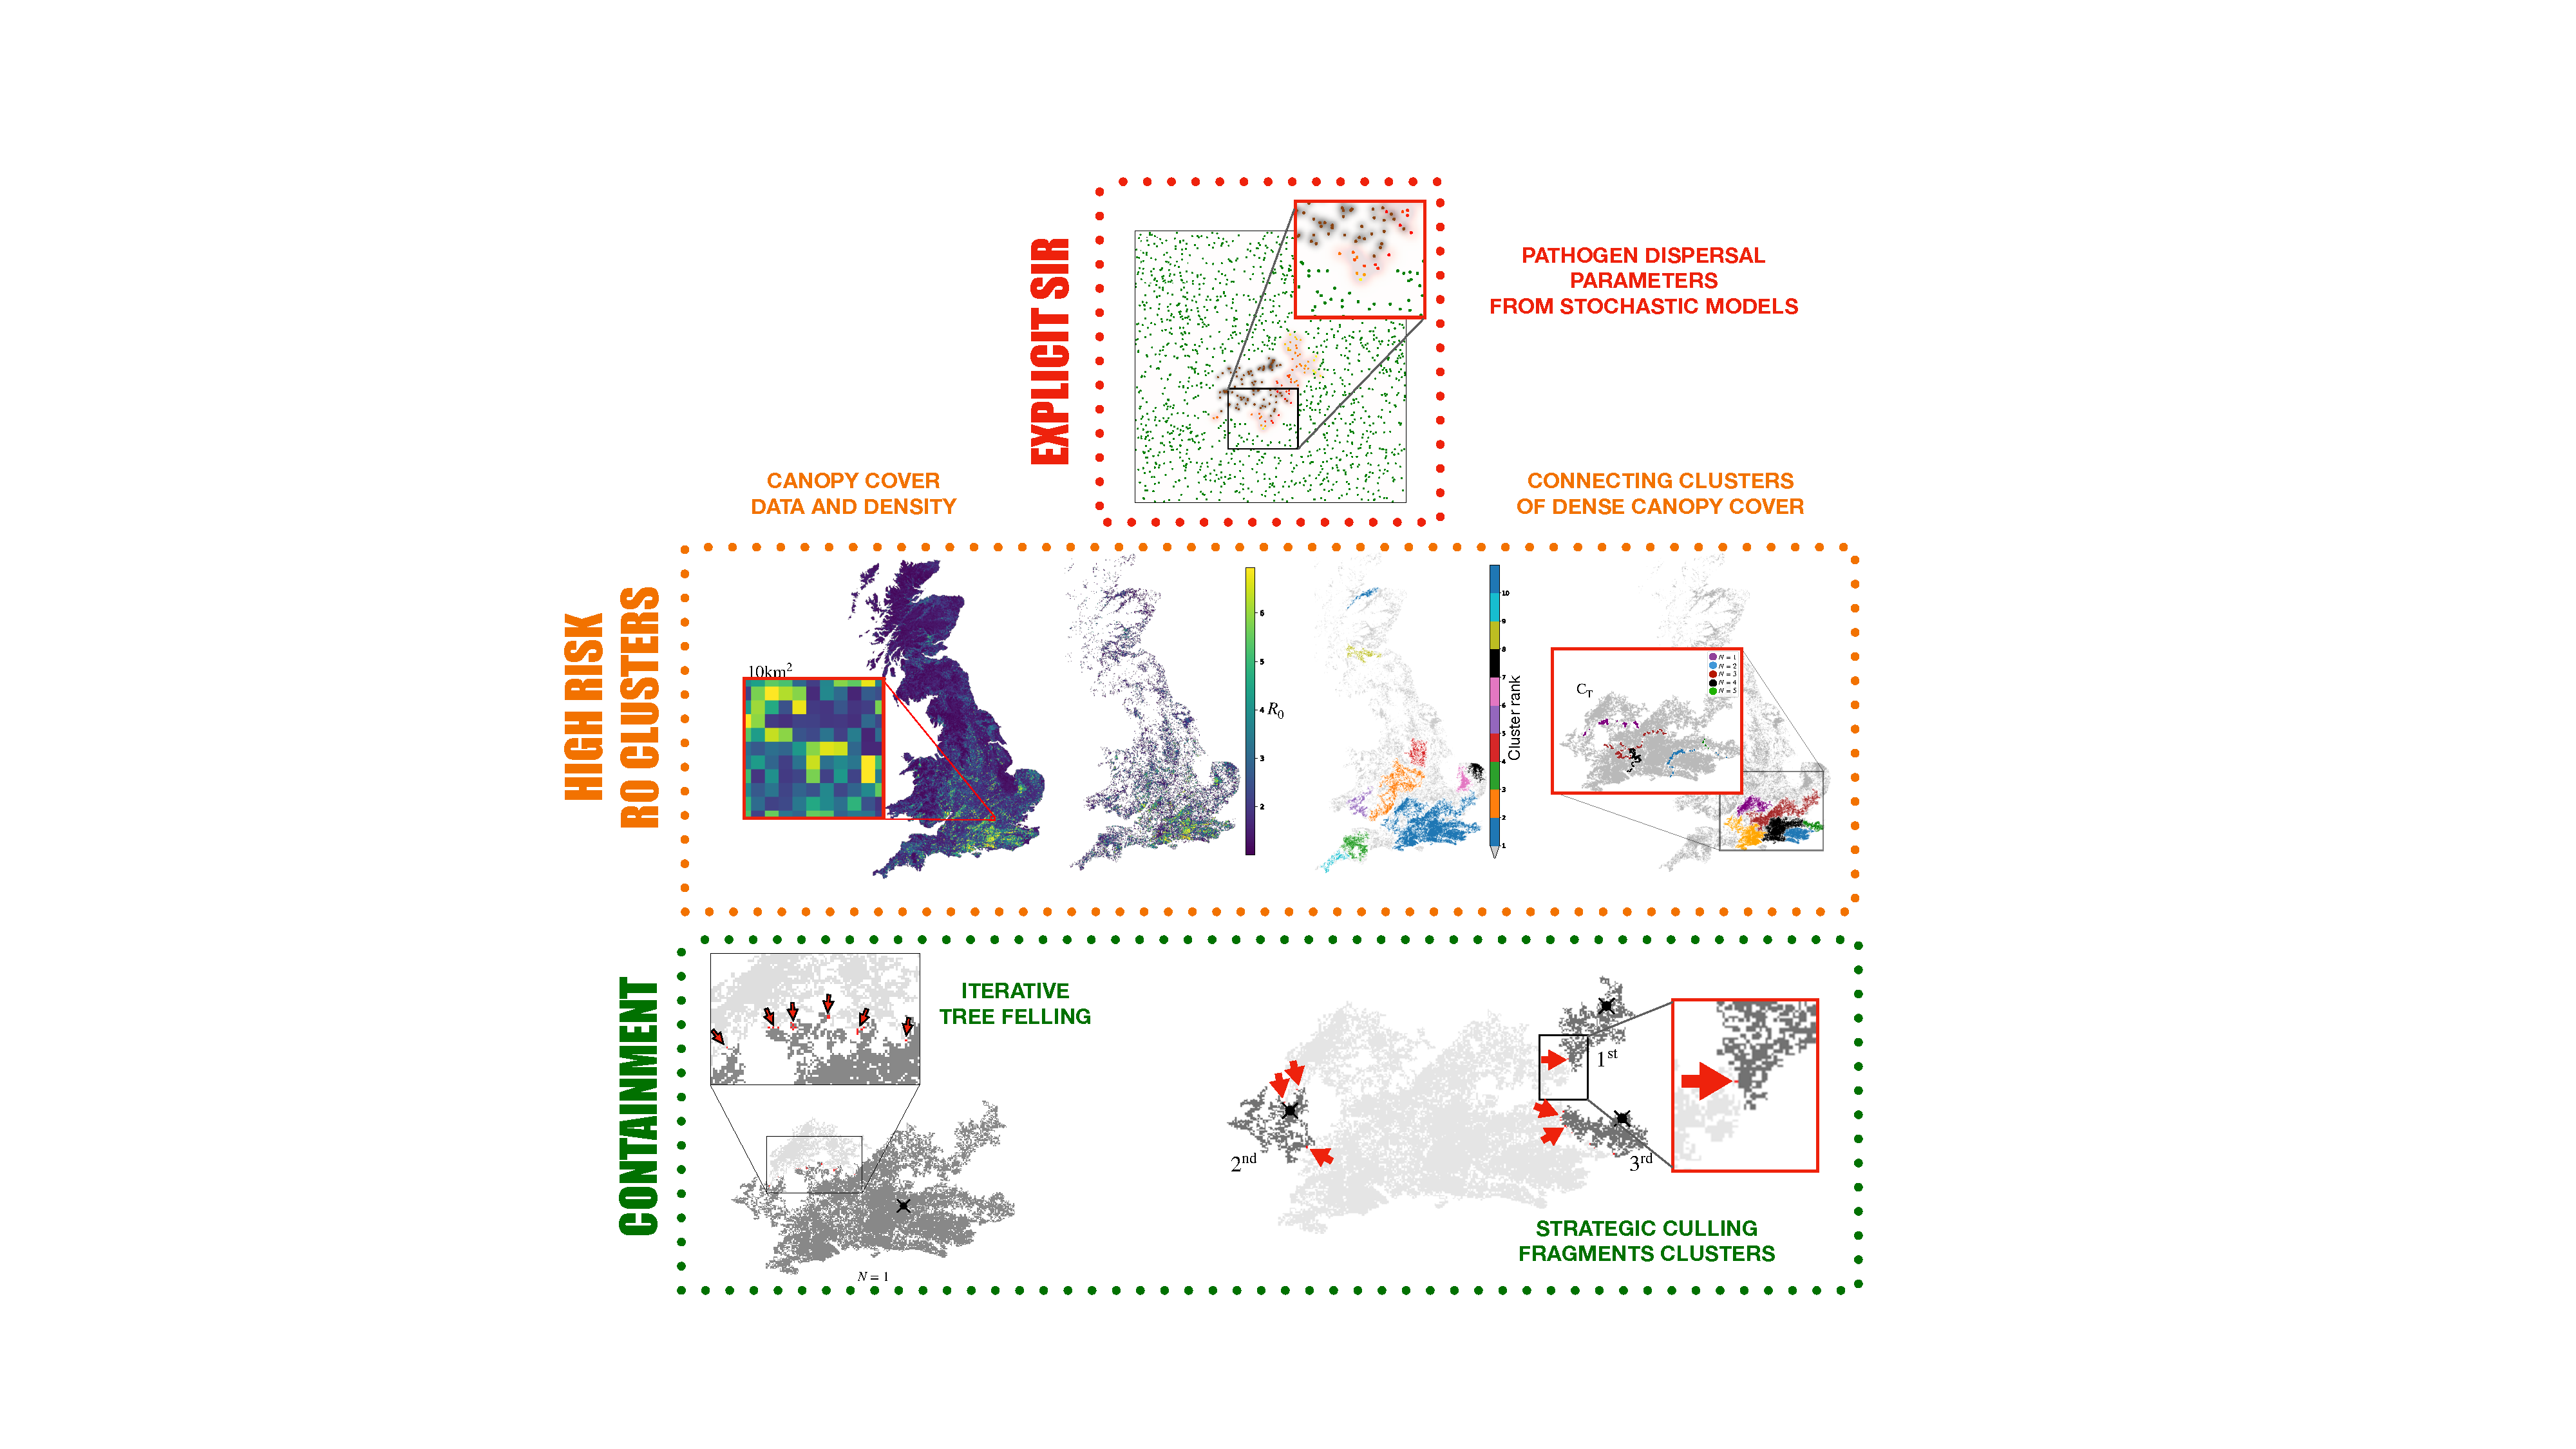
\includegraphics[scale=0.5]{appendix/Graphical_Abstract.pdf}
    \caption{Caption}
    \label{fig:my_label}
\end{figure}






% ------------------------------------------------------------------------------
% Reference list
% ------------------------------------------------------------------------------


% \bibliographystyle{apalike}
\bibliographystyle{acm}
\bibliography{references}
\end{document}
